% ---------------------------------------------------------------------------- %

\documentclass[10pt,dvipsnames]{article}
\usepackage[a4paper,left=3cm,right=3cm,top=2.5cm,bottom=3.25cm]{geometry}
\usepackage{fontspec}
\usepackage{polyglossia}
\usepackage{setspace}
\usepackage{lipsum}
\usepackage{fontspec}
\usepackage{titlesec}
\usepackage{parskip}
\usepackage{amsmath}
\usepackage{unicode-math}
\usepackage{url}
\usepackage{suffix}
\usepackage{pdfpages}
\usepackage{enumitem}
\usepackage{fancyvrb}
\usepackage{minted}
\usepackage{tabularx}
\usepackage{etoolbox}
\usepackage{xpatch}
\usepackage{xspace}
\usepackage{calc}
\usepackage{multirow}
\usepackage{booktabs}
\usepackage{xcolor}
\usepackage{csquotes}
\usepackage{pdflscape}
\usepackage{graphicx}
\usepackage[htt]{hyphenat}
\usepackage[section]{placeins} % keep floats in the section where they are decl.
\usepackage[labelfont=bf]{caption}
\usepackage[tocfullflat]{tocstyle}
\usepackage[hidelinks]{hyperref}
\usepackage[backend=bibtex,style=authoryear,dashed=false]{biblatex}

% ---------------------------------------------------------------------------- %
% prerequisites

% This template works great on Overleaf!

% This template requires XeTeX and the Arial and Courier New fonts. On
% Debian-based systems (e.g., Ubuntu), these can be installed by typing the
% following commands:

%   $ sudo apt update
%   $ sudo apt install ttf-mscorefonts-installer
%   $ wget http://ftp.us.debian.org/debian/pool/contrib/m/msttcorefonts/ttf-mscorefonts-installer_3.6_all.deb
%   $ sudo dpkg -i ttf-mscorefonts-installer_3.6_all.deb

% ---------------------------------------------------------------------------- %
% conform to word template

\setmainfont{Arial}
\setmonofont{Courier New}

\linespread{1.5}
\setlength{\parskip}{\baselineskip}

\raggedbottom

\titlelabel{\thetitle.\quad}

\titleformat*{\section}{\fontsize{18pt}{\baselineskip}\bfseries}
\titleformat*{\subsection}{\fontsize{16pt}{\baselineskip}\bfseries}
\titleformat*{\subsubsection}{\fontsize{14pt}{\baselineskip}\bfseries}

\titlespacing{\section}{0pt}{0pt}{0pt}
\titlespacing{\subsection}{0pt}{0pt}{0pt}
\titlespacing{\subsubsection}{0pt}{0pt}{0pt}

\let\oldsection\section
\let\oldsubsection\subsection
\let\oldsubsubsection\subsubsection

\newcommand{\mysection}[1]{
  \clearpage
  \vspace*{2.25cm}
  \oldsection{#1}
  \vspace{0.42cm}
}

\newcommand{\mysectionstar}[1]{
  \clearpage
  \vspace*{2.25cm}
  \oldsection*{#1}
  \vspace{0.42cm}
}

\makeatletter
\renewcommand{\section}{\@ifstar{\mysectionstar}{\mysection}}
\makeatother

\renewcommand{\subsection}[1]{\vspace{1.06cm}\oldsubsection{#1}\vspace{0.11cm}}
\renewcommand{\subsubsection}[1]{\vspace{0.85cm}\oldsubsubsection{#1}\vspace{0.11cm}}

\setdefaultlanguage{portuges}

\addto\captionsportuges{
  \renewcommand{\contentsname}{Índice}
  \renewcommand{\listfigurename}{Índice de Figuras}
  \renewcommand{\listtablename}{Índice de Tabelas}
}

\usetocstyle{standard}
\newcommand{\autodot}{.}

\setenumerate{noitemsep}
\setitemize{noitemsep}

\renewcommand{\arraystretch}{1.25}

% maintain definition order between figures and tables in output
\makeatletter
\let\ftype@table\ftype@figure
\makeatother

\addbibresource{bibliography.bib}
\setlength\bibitemsep{\baselineskip}
\renewcommand*{\nameyeardelim}{\addcomma\space}

\DeclareMathSizes{10}{10}{10}{10}

% ---------------------------------------------------------------------------- %
% small optional style configurations

\renewcommand\labelitemi{--}

\definecolor[named]{ACMDarkBlue}{cmyk}{1,0.58,0,0.21}

\hypersetup{
    hidelinks,
    colorlinks,
    linkcolor=black,
    citecolor=black,
    urlcolor=ACMDarkBlue,
    filecolor=ACMDarkBlue
    }

\setlength{\tabcolsep}{6pt}
\renewcommand{\arraystretch}{1.4}

\setlength{\textfloatsep}{20.0pt plus 2.0pt minus 4.0pt}
\setlength{\floatsep}{20.0pt plus 2.0pt minus 2.0pt}
\setlength{\intextsep}{20.0pt plus 2.0pt minus 2.0pt}

\newcommand{\tabelausecase}{\small}

% ---------------------------------------------------------------------------- %
% utilities

\newcommand{\itemizedpar}[1]{\vspace*{-\baselineskip}\paragraph{\emph{#1}}}
% \newcommand{\rubric}[1]{\noindent{\textbf{#1}}}
\newcommand{\inlineenum}[1]{(#1)}

\newcommand{\verttext}[1]{\parbox[t]{2mm}{\rotatebox[origin=c]{90}{\ \ #1\ \ }}}

\newcommand{\refcap}[1]{\hyperref[#1]{Capítulo~\ref*{#1}}}
\newcommand{\refsec}[1]{\hyperref[#1]{Secção~\ref*{#1}}}
\newcommand{\refane}[1]{\ref{#1}}
\newcommand{\reffig}[1]{\hyperref[#1]{Figura~\ref*{#1}}}
\newcommand{\reftab}[1]{\hyperref[#1]{Tabela~\ref*{#1}}}

\makeatletter
\AtBeginEnvironment{minted}{\dontdofcolorbox}
\def\dontdofcolorbox{\renewcommand\fcolorbox[4][]{##4}}
\xpatchcmd{\inputminted}{\minted@fvset}{\minted@fvset\dontdofcolorbox}{}{}
\makeatother

\setminted{
  autogobble,
  breaklines,
  baselinestretch=1.2,
  frame=leftline,
  framesep=8pt,
  xleftmargin=7pt
  }

% ---------------------------------------------------------------------------- %
% comments

\newcommand{\mynote}[3]{
   \fbox{\bfseries\sffamily\scriptsize#1}
   {\small$\blacktriangleright$\textsf{\emph{\color{#2}{#3}}}$\blacktriangleleft$}}

\newcommand{\alberto}[1]{\mynote{alberto}{red}{#1}}
\newcommand{\cesar}[1]{\mynote{cesar}{red}{#1}}
\newcommand{\fabio}[1]{\mynote{fabio}{red}{#1}}
\newcommand{\guilherme}[1]{\mynote{guilherme}{red}{#1}}
\newcommand{\luis}[1]{\mynote{luis}{red}{#1}}

% ---------------------------------------------------------------------------- %
% document

\begin{document}


\includepdf[pages=-]{cover/cover.pdf}

% ---------------------------------------------------------------------------- %

\section*{Resumo}
\pagenumbering{roman}

Este documento consiste no relatório correspondente ao trabalho prático realizado no âmbito da Unidade Curricular de Laboratórios de Informática IV, do curso de Mestrado Integrado em Engenharia Informática da Universidade do Minho, no ano letivo de 2018/2019. Considera-se o caso de estudo do desenvolvimento do assistente pessoal de cozinha \emph{Bela Sopa}, a pedido da cadeia de supermercados e hipermercados \emph{Gota Doce}.

É primeiramente fundamentada a construção do sistema tendo em conta a sua utilidade e viabilidade, elaborando-se também um plano para o seu desenvolvimento. O processo de especificação do sistema é em seguida pormenorizado, apresentando-se com particular detalhe os resultados das fases de modelação de domínio, levantamento e análise de requisitos, modelação de \emph{use cases}, prototipagem da interface de utilizador e modelação da arquitetura interna do sistema. É por fim descrito o processo de construção do mesmo e apresentado o produto resultante.

% ---------------------------------------------------------------------------- %

\paragraph{Área de Aplicação:}

Desenvolvimento de sistemas de software.

% ---------------------------------------------------------------------------- %

\vspace*{-\baselineskip}
\paragraph{Palavras-Chave:}

Culinária;
Assistente pessoal de cozinha;
Sistemas de software;
Engenharia de software.

% ---------------------------------------------------------------------------- %


\tableofcontents

{
  \usetocstyle{allwithdot}
  \renewcommand{\baselinestretch}{0.9}
  \normalsize
  \listoffigures
  \listoftables
}

\renewcommand{\mysectionstar}[1]{
  \clearpage
  \vspace*{2.25cm}
  \phantomsection
  \oldsection*{#1}
  \addcontentsline{toc}{section}{#1}
  \vspace{0.42cm}
}

% ---------------------------------------------------------------------------- %

\section{Introdução}
\label{cap:introducao}
\pagenumbering{arabic}

Este relatório documenta o trabalho desenvolvido no âmbito da Unidade Curricular de Laboratórios de Informática IV, do curso de Mestrado Integrado em Engenharia Informática da Universidade do Minho, no ano letivo de 2018/2019.

O caso de estudo considerado centra-se no desenvolvimento do assistente pessoal de cozinha \emph{Bela Sopa}, sucessor ao serviço \emph{online} intitulado \emph{Escola de Cozinha} disponibilizado pela cadeia de supermercados e hipermercados portuguesa \emph{Gota Doce}. Este capítulo contextualiza e apresenta o caso de estudo, descrevendo também as motivações e os objetivos do projeto, e delineia a estrutura do presente relatório.

% ---------------------------------------------------------------------------- %

\subsection{Contextualização e caso de estudo}
\label{sec:introducao:contextualizacao}

O \emph{Gota Doce} é uma cadeia de supermercados e hipermercados portuguesa, sediada em Lisboa. Foi fundada em 1983 pelo grupo empresarial \emph{Merónimo Jartins} em colaboração com a empresa belga \emph{Gelhaize Droup}. A cadeia possui atualmente mais de 400 lojas físicas distribuídas por cerca de 290 localidades portuguesas, contando com aproximadamente 32 milhares de colaboradores e 700 mil visitas diárias.

Além desta vasta rede de pontos de serviço, a empresa \emph{Gota Doce} oferece também vários serviços \emph{online}, destacando-se o serviço de entrega de produtos ao domicílio. Outros serviços têm como objetivo a fidelização de clientes e a manutenção da imagem da marca, como é o caso da \emph{Escola de Cozinha}, uma plataforma \emph{online} que disponibiliza informação relacionada com culinária. Esta oferece auxílio à confeção de refeições por parte dos seus utilizadores, fornecendo principalmente descrições estáticas de receitas, técnicas de cozinha e ingredientes.

Sendo este serviço utilizado por uma quantidade considerável de clientes da cadeia \emph{Gota Doce}, a empresa pretende agora investir na melhoria da plataforma, focando a possibilidade de adaptação e personalização do serviço a cada um dos seus utilizadores. Com esse objetivo, foi pedido o desenvolvimento de um assistente pessoal de cozinha que substituirá o atual serviço \emph{Escola de Cozinha}. Por forma a se provar a viabilidade e adequação desta nova plataforma, a sua versão inicial será dedicada exclusivamente à confeção de sopas. O caso de estudo no qual o trabalho documentado neste relatório se baseia corresponde então ao desenvolvimento do assistente em causa, intitulado \emph{Bela Sopa}.

% Para além desta vasta disponibilidade de pontos de serviço, com as várias lojas apresentadas em diversos pontos do país, o \emph{Gota Doce} também oferece os seus serviços \emph{online} através do seu \emph{website}. Os clientes podem assim usufruir do serviço de compras \emph{online}, o qual permite o acesso aos seus produtos de uma forma mais abrangente e conveniente.

% Embora o \emph{website} sirva como uma extensão do alcance dos seus serviços de venda de produtos, o \emph{Gota Doce} decidiu fornecer outros serviços, entre os quais se encontra presente a plataforma \emph{Escola de Cozinha}.

% A \emph{Escola de Cozinha} é uma plataforma que procura transmitir conhecimento que ajuda os utilizadores da mesma a confecionar variadas refeições, a aumentar o seu domínio culinário e a incentivar a confeção de refeições caseiras.

% De acordo com as características dos seus conteúdos, a \emph{Escola de Cozinha} divide-os em 5 secções: técnicas, ingredientes, vídeos, receitas e histórias de cozinha.

% \itemizedpar{Técnicas.}

% Nesta secção são apresentadas receitas nas quais são introduzidas técnicas que requerem alguma experiência, ou que merecem ser realçadas. Para facilitar a aprendizagem destas técnicas estas são apresentadas em conjunto com imagens que ilustram detalhadamente os passos a tomar em cada estágio.

% \itemizedpar{Ingredientes.}

% Nesta secção diversos ingredientes são descritos em detalhe, desta forma o utilizador poderá conhecer melhor o ingrediente e desta forma conseguir incluir o mesmo nas sua refeições.

% \itemizedpar{Vídeos.}

% Contém diversos vídeos nos quais são demonstradas técnicas e confecionadas receitas, desta forma os utilizadores têm uma maior facilidade na compreensão das técnicas e passos presentes nas receitas.   

% \itemizedpar{Receitas.}

% São apresentadas diversas receitas, cada uma caraterizada por dificuldade (fácil, média, difícil) e tempo de confeção, tipo de prato (entrada, sobremesa, etc) e número de porções, isto é, para quantas pessoas é a receita. Para além dessa caraterização, é apresentada uma descrição do prato e são também descritos os procedimentos passo a passo, para confecionar o prato, conjuntamente com a lista de ingredientes e medidas dos mesmos, tabela de valores nutricionais.

% \itemizedpar{Histórias de cozinha.} 

% Constitui um conjunto de artigos que fornecem um complemento informativo na cultura culinária do utilizador. Os assuntos abordados englobam as componentes estéticas e técnicas da cozinha, fornecendo um contributo para as habilidades culinárias do utilizador.

% A \emph{Escola de Cozinha} tem registado um grande volume de visitas, desde a sua introdução e em analise verificou-se um aumento do número de clientes e produtos adquiridos através da loja online do \emph{Gota Doce}. Devido a este sucesso foi decidido o investimento na melhoria da \emph{Escola de Cozinha} para continuar a explorar essa possibilidade de aumento de negócio.

% Com essa ideia em mente, o \emph{Gota Doce} abordou-nos e após discussão de ideias surgiu a aplicação \emph{Bela Sopa}, um assistente pessoal de cozinha, através de uma tentativa de adaptar e personalizar o serviço a cada um dos utilizadores.

% Como fase inicial o assistente pessoal de cozinha apenas irá ajudar à confeção de sopas de forma a estudar melhor a receção desta nova aplicação por parte do público, sem ser necessário um orçamento elevado. Através desta limitação do âmbito da aplicação é possível a ampliação das funcionalidades da aplicação para que a quando a migração dos restantes conteúdos a aplicação já se apresente a um nível de qualidade elevado.

% ---------------------------------------------------------------------------- %

\subsection{Motivação e objetivos}
\label{sec:introducao:motivacao-objetivos}

Embora não se pretenda monetizar diretamente a plataforma em questão (\emph{e.g.}, através de subscrições pagas para acesso aos serviços por esta disponibilizados), objetiva-se com a sua construção angariar e fidelizar clientes para os principais serviços oferecidos pela empresa \emph{Gota Doce}. A título de exemplo, o sistema poderá promover a utilização desses outros serviços ao indicar que os ingredientes utilizados por uma determinada receita podem ser obtidos em lojas físicas \emph{Gota Doce} próximas ou através do serviço de entrega ao domicílio disponibilizado pela empresa. A plataforma poderá também aumentar a exposição dos clientes da cadeia a folhetos promocionais e outros materiais publicitários.

De forma geral e sumária, pretende-se que a construção da plataforma em questão contribua para o crescimento e manutenção do volume de negócio da empresa \emph{Gota Doce}. Estes objetivos serão detalhados e quantificados em secção posterior deste relatório.

% O cliente decidiu iniciar este projeto com o intuito de criar uma relação mais íntima com os seus clientes, de suavizar o acesso às suas receitas no seu \emph{website} e promover os seus produtos e o serviço de entrega ao domicílio. Com este projeto espera-se aumentar o numero de compras de produtos da marca \emph{Gota Doce}, o reconhecimento e divulgação da marca, o que leva a uma maior atração de clientes e consequentemente um maior lucro.

% ---------------------------------------------------------------------------- %

\subsection{Estrutura do relatório}
\label{sec:introducao:estrutura-relatorio}

Este documento apresenta a seguinte estrutura:

\begin{itemize}

  \item No \refcap{cap:fundamentacao} fundamenta-se o sistema, tendo em conta a sua utilidade e viabilidade e justificando-se o seu desenvolvimento;
  
  \item No \refcap{cap:planeamento} é apresentado o planeamento do projeto, juntamente com um modelo inicial do sistema, recursos necessários à concretização do mesmo, medidas de sucesso e um plano detalhado do seu desenvolvimento;
  
  \item No \refcap{cap:dominio} inicia-se a fase de especificação do sistema descrevendo-se o processo de modelação de domínio e os respetivos resultados;
  
  \item No \refcap{cap:requisitos} apresenta-se o levantamento e análise de requisitos, enumerando-se os requisitos identificados e efetuando-se uma análise geral dos mesmos;
  
  \item No \refcap{cap:use-cases} procede-se à modelação de \emph{use cases}, começando-se por identificar a totalidade dos \emph{use cases} considerados e apresentando-se depois a sua especificação;
  
  \item No \refcap{cap:interface} é executada a prototipagem da interface de utilizador do sistema, recorrendo-se primariamente a esquemas do seu aspeto gráfico;
  
  \item No \refcap{cap:arquitetura} apresenta-se e especifica-se de forma holística a arquitetura interna do sistema;
  
  \item No \refcap{cap:dados} detalha-se a especificação da camada de dados do sistema, modelando-se também a base de dados subjacente;
  
  \item No \refcap{cap:negocio} especifica-se da camada de negócio do sistema recorrendo primariamente a diagramas de classes e de sequência;
  
  \item No \refcap{cap:construcao} descreve-se a fase de construção do sistema, apresentando-se também o produto resultante;
  
  \item No \refcap{cap:conclusao} o relatório é concluído com um resumo do processo de desenvolvimento do sistema e com a identificação de trabalho futuro.

\end{itemize}

Adicionalmente, são incluídos dois anexos:

\begin{itemize}

  \item No \refane{ane:use-cases-spec} são reproduzidas as especificações de todos os \emph{use cases} identificados no \refcap{cap:use-cases};

  % \item No \refane{ane:dados-sbd-concetual} são descritas as entidades, relacionamentos e atributos do modelo concetual do sistema de bases de dados descrito na \refsec{sec:dados:sbd:concetual};

  % \item No \refane{ane:dados-diag-seq} são incluídos todos os diagramas de sequências desenvolvidos relativos à camada de dados descrita no \refcap{cap:dados};

  \item No \refane{ane:negocio-diag-seq} são incluídos todos os diagramas de sequência relativos à camada de negócio descrita no \refcap{cap:negocio}.

\end{itemize}
  
% ---------------------------------------------------------------------------- %

% ---------------------------------------------------------------------------- %

\section{Fundamentação do Sistema}
\label{cap:fundamentacao}

Tendo-se apresentado o caso de estudo e identificado as motivações e objetivos para o desenvolvimento do sistema em questão, este capítulo define agora a sua identidade e fundamenta a sua construção tendo em conta a viabilidade e utilidade do mesmo.

% ---------------------------------------------------------------------------- %

\subsection{Identidade do sistema}
\label{sec:fundamentacao:identidade}

O \emph{Bela Sopa} consiste num assistente pessoal que tem como objetivo acompanhar o utilizador durante todo o processo de confeção de uma receita de sopa, destinando-se à faixa etária adulta e não sendo direcionado a menores de idade.

Durante a confeção da receita, o assistente é capaz de interagir com o utilizador, designando quais os ingredientes necessários e os passos serem a executados, proporcionando também informação relativa aos utensílios e técnicas a utilizar durante a produção do prato, sendo assim capaz de responder a diferentes cenários alternativos.

Várias caraterísticas que definem a identidade do sistema são apresentadas na \reftab{tab:fundamentacao:identidade}.

\begin{table}[ht]
  \centering
  \begin{tabular}{ | l | l | }
    \hline
    \textbf{Nome} & \emph{Bela Sopa} \\ \hline
    \textbf{Categoria} & Assistente pessoal \\ \hline
    \textbf{Designação} & Assistente pessoal de cozinha para a confeção de sopas \\ \hline
    \textbf{Idioma} & Português \\ \hline
    \textbf{Faixa etária} & Adultos \\ \hline
    \textbf{Características} & \emph{User friendly}, personalizável e prático\\ \hline
    \textbf{Empresa cliente} & \emph{Gota Doce} \\ \hline
  \end{tabular}
  \caption{Ficha de projeto.}
  \label{tab:fundamentacao:identidade}
\end{table}

% ---------------------------------------------------------------------------- %

\subsection{Justificação, viabilidade e utilidade do sistema}
\label{cap:fundamentacao:justificacao}

Justifica-se a realização deste projeto para substituir o serviço \emph{Escola de Cozinha} por um sistema interativo, eficiente, inteligente e de melhor qualidade. Com este projeto a nossa empresa obtém um cliente de grande escala enquanto que o cliente obtém um serviço inovador.

Antes do nosso cliente ter investido neste projeto, teve que ter um contexto para o mesmo. Para isso, este teve de investigar os seus clientes atuais e desejados para entender a vida dos mesmos e as suas necessidades, ficando com uma ideia do futuro do projeto para atender às demandas dos seus clientes.

Isto foi feito através de um questionário, o qual se concluiu que cerca de 80\% das pessoas, tanto clientes atuais como possíveis futuros clientes, procuram respostas tecnológicas aos seus problemas diários, e que 70\% destes utilizariam um assistente pessoal para ajudar na sua culinária, enquanto que apenas 8\% possuem elevada experiência culinária. 

Este projeto é viável pelas seguintes razões:

\begin{itemize}

    \item Não existem obstáculos legais (leis ou patentes) que proíbam ou limitem o desenvolvimento e comercialização do produto resultante;
    
    \item A nossa equipa prevê que o desenvolvimento deste produto é exequível com os recursos tecnológicos atuais;
    
    \item É geograficamente favorável devido ao elevado número de super e hipermercados e à sua dispersão pelo território nacional;
    
    \item É vantajoso em termos de visibilidade pública, uma vez que a cadeia \emph{Gota Doce} está associada ao produto;
    
    \item Não existe impactos ambientais associados ao produto;
    
    \item Financeiramente, prevê-se que o projeto seja rentável a curto prazo.
    
\end{itemize}

% ---------------------------------------------------------------------------- %

% ---------------------------------------------------------------------------- %

\section{Planeamento do Projeto}
\label{cap:planeamento}

Estando fundamentada a construção do assistente \emph{Bela Sopa}, apresenta-se agora o planeamento do seu desenvolvimento. Começa-se por se definir um modelo inicial do sistema, procedendo-se com a identificação de recursos necessários à sua concretização e de medidas de sucesso. Por fim, apresenta-se um plano cronológico detalhado do seu desenvolvimento.

% ---------------------------------------------------------------------------- %

\subsection{Maqueta do sistema}
\label{cap:planeamento:maqueta}

Embora não seja ainda possível determinar o conjunto exato de funcionalidades desejadas e a estrutura interna do sistema a ser desenvolvido, podem já ser identificados os seus principais tipos de utilizador e componentes, assim como possíveis dependências em serviços externos.

\begin{figure}[ht]
  \centering
  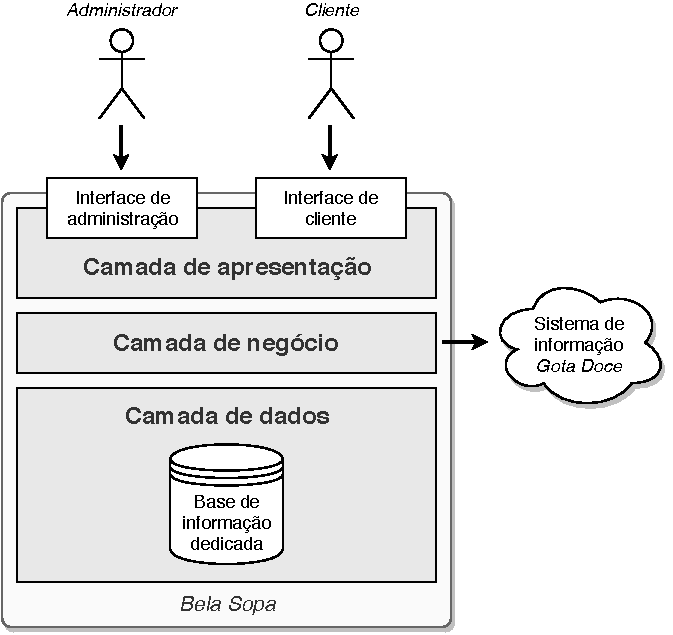
\includegraphics{figures/03/maqueta.pdf}
  \caption{Maqueta do sistema.}
  \label{fig:planeamento:maqueta}
\end{figure}

Com base nessa informação, foi elaborado um modelo inicial do sistema (ou \emph{maqueta}), o qual é apresentado na \reffig{fig:planeamento:maqueta}. Identificam-se dois tipos de utilizador: \emph{administradores} --- responsáveis pela gestão dos conteúdos disponibilizados --- e \emph{clientes} --- correspondentes ao público-alvo do sistema \emph{Bela Sopa}. Na figura, a entidade ou componente na origem de cada seta inicia interações com o componente no destino da mesma.

Prevê-se a possibilidade de a plataforma fazer uso de um sistema de informação detido pela empresa \emph{Gota Doce} por forma a obter dados sobre produtos e lojas da mesma e a tirar partido da base de informação relativa a receitas culinárias e ingredientes atualmente em uso pelo serviço \emph{Escola de Cozinha}. No entanto, prevê-se também que a plataforma necessite de uma base de informação própria, dedicada à gestão de dados específicos ao serviço a ser desenvolvido.

Explicita-se que este modelo é provisório e não vinculativo, tendo o principal objetivo de auxiliar a identificação de recursos necessários ao desenvolvimento do sistema e o início da fase de especificação do mesmo.

% ---------------------------------------------------------------------------- %

\subsection{Recursos necessários}
\label{sec:planeamento:recursos}

%\begin{itemize}
%  \item Não é ``computadores e software''.
%  \item Recursos importantes para garantir o %sucesso do desenvolvimento do sistema.
%  \item Equipa de desenvolvimento.
%  \item E equipa que nos dá o conhecimento %necessário (em culinária).
%\end{itemize}

Estabeleceu-se que, para o desenvolvimento do sistema, é necessária uma equipa de desenvolvimento de 8 elementos, respetivamente, 1 gestor, 1 analista, 4 programadores e 2 engenheiros de software.

Para além disso, será necessário utilizar os recursos disponibilizados pela empresa \emph{Gota Doce}, como a base de receitas da plataforma \emph{Escola de Cozinha}, por forma a obter o nome das receitas, a dificuldade, a duração, os ingredientes, os passos da receita e as porções concebidas para as sopas, e um consultor que nos dará a informação necessária sobre culinária.

% ---------------------------------------------------------------------------- %

\subsection{Medidas de sucesso}
\label{sec:planeamento:medidas-sucesso}

% \alberto{Sugestão: Ter \textbf{\emph{lista}} de medidas de sucesso sucintas, objetivas e quantitativas.}

As medidas de sucesso aqui enumeradas foram estabelecidas através de uma reunião entre o nosso gestor e a equipa de contabilidade do nosso cliente, sendo que os dados referidos foram especulados com base em 6 meses de uso do sistema após o seu lançamento.

Estima-se que:

\begin{itemize}
    
    \item A venda de produtos aumente em, pelo menos, 5\% através da utilização do sistema;
    
    \item O sistema seja utilizado em média por 1000 utilizadores distintos por dia;
    
    \item O número de clientes da cadeia aumente em, pelo menos, 3\%;
    
    % \item Assegure os clientes atuais que estão bem servidos;
    
    % \item Um aumento 10\% na procura de produtos e 5\% nos pedidos via online que por consequente aumenta 3\% a utilização do serviço entrega ao domicílio.

    \item O número de pedidos efetuados através do serviço de entrega ao domicílio aumente em, pelo menos, 10\%.

\end{itemize}

% ---------------------------------------------------------------------------- %

\subsection{Plano de desenvolvimento}
\label{sec:planeamento:plano-desenvolvimento}

% \begin{itemize}
%   \item Diagrama de Gantt -- Microsoft Project.
%   \item Distribuição de trabalho por pessoa? (???)
%   \item Quantidade de horas de trabalho.
%   \item Assumir trabalhar ao dia, dias de 8 horas.
%   \item Dá depois para contabilizar o quanto vamos gastar a desenvolver o projeto ("era engraçado fazerem isso").
%   \item E.g.: contabilizar tempo para falar com consultor (por exemplo, chef). Uma semana chega, faz de conta, e vamos levar 2 pessoas para falar.
%   \item Convém manter Gantt original no relatório final.
% \end{itemize}

\begin{figure}[ht]
  \centering
  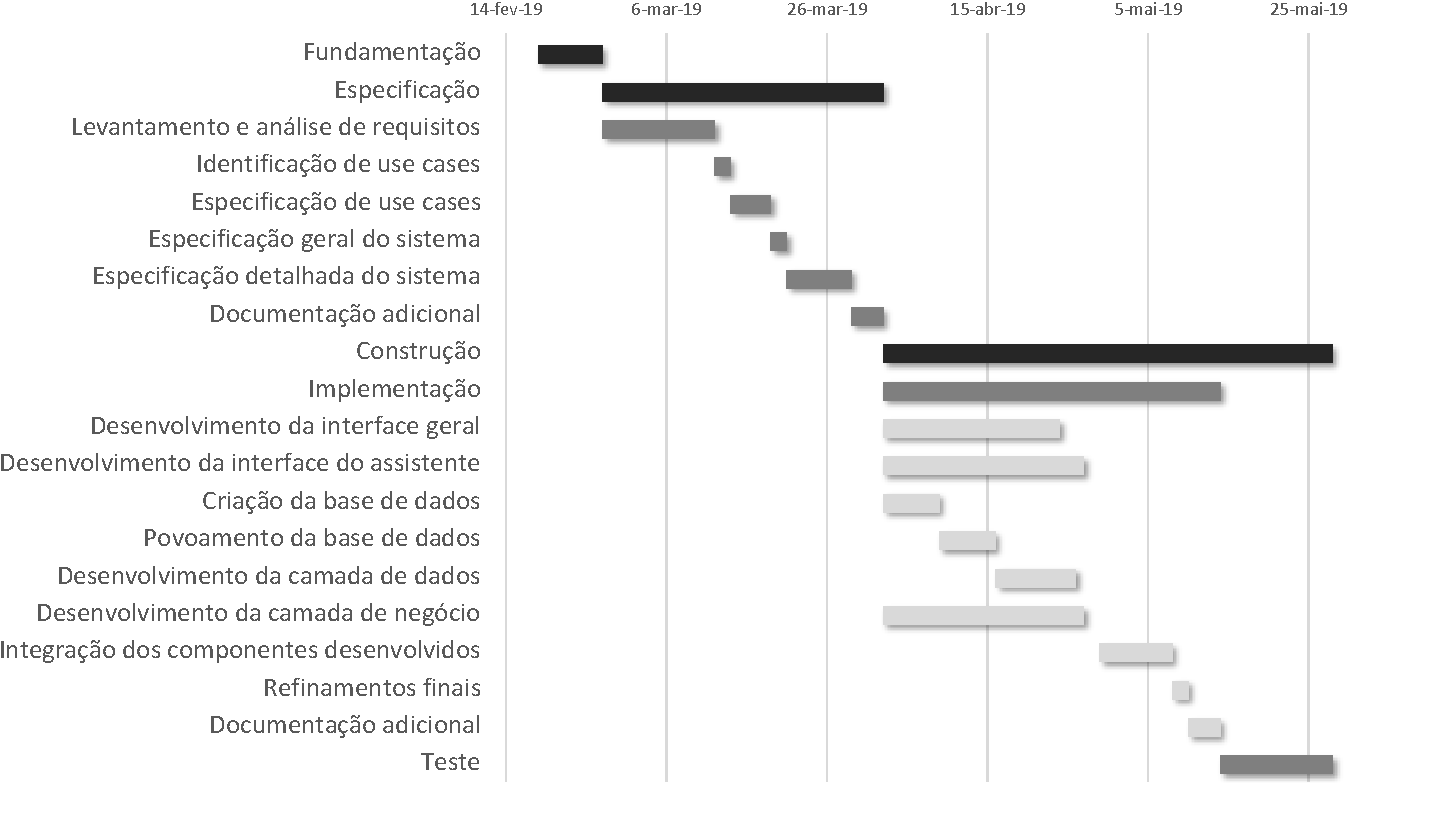
\includegraphics[width=\textwidth]{figures/03/planeamento-gantt.pdf}
  \caption{Diagrama de Gantt para o desenvolvimento do projeto.}
  \label{fig:planeamento:gantt}
\end{figure}

A análise e fundamentação do projeto será feita pelo analista da equipa, e os restantes processos só serão feitos após esta fase, com uma duração de 6 dias.

Durante o desenvolvimento do sistema estimam-se 6 tarefas necessárias, respetivamente, levantamento de requisitos, análise de requisitos, arquitetura de software, testes e implementação.
O gestor e os colaboradores correspondentes à fase atual do projeto, irão se reunir duas vezes por semana de forma a distribuir tarefas para permitir trabalho autónomo e debater eventuais dúvidas, conflitos ou problemas no trabalho a realizar.

O levantamento de requisitos e sua respetiva análise terá a duração de 3 dias e será realizado pelos engenheiros de software e com o auxilio de um consultor ainda a ser disponibilizado pelo \emph{Gota Doce}.

A identificação e especificação de use cases demorará 4 dias e será feito após o levantamento e análise de requisitos. A arquitetura de software terá um espaço de 4 semanas e será realizada pelos engenheiros de software. A implementação terá a duração de 6 semanas e será realizada pelos programadores.

Os testes serão feitos durante 10 dias por um programador da equipa de desenvolvimento e um outro programador que desconhece o produto, de forma a que os testes sejam feitos de forma imparcial e independentes do facto do colaborador ter desenvolvido o produto ou não. Após isto, durante 4 dias será realizada a apresentação e instalação do sistema de software nos ambientes do cliente.

Em suma, estimam-se 14 semanas para o desenvolvimento deste sistema.

O custo associado a cada uma das fases do projeto encontra-se na Figura \ref{fig:planeamento:custosgerais}, estando associado ao custo inicial a fase "Análise e fundamentação". Em suma o custo total do projeto é de 30.052,00 euros.

\begin{figure}[ht]
  \centering
  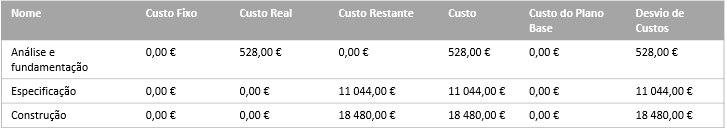
\includegraphics[width=\textwidth]{figures/03/planeamento-custos.png}
  \caption{Custos associados a cada fase do projeto.}
  \label{fig:planeamento:custosgerais}
\end{figure}

Estes custos foram gerados tendo em conta 8 horas de trabalho por dia, 5 dias por semana, e os custos para cada elemento individualmente que se encontram na \reffig{fig:planeamento:recursoshumanos}.

\begin{figure}[ht]
  \centering
  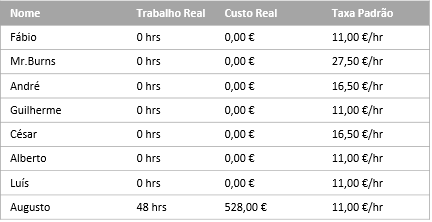
\includegraphics[scale=1.15]{figures/03/planeamento-recursos.png}
  \caption{Custos associados a cada contribuidor do projeto.}
  \label{fig:planeamento:recursoshumanos}
\end{figure}

% ---------------------------------------------------------------------------- %

% ---------------------------------------------------------------------------- %

\section{Modelação de Domínio}
\label{cap:dominio}

Verificou-se que a construção do sistema seria vantajosa para a empresa e que o seu processo de desenvolvimento cumpriria o orçamento e prazos estabelecidos, reunindo-se assim as condições necessárias para se proceder à fase de especificação do mesmo.

Embora os procedimentos de modelação de domínio e de levantamento de requisitos sejam mutuamente dependentes, apresenta-se em primeiro lugar neste relatório o modelo de domínio por forma a clarificar a enunciação dos requisitos apresentados no próximo capítulo.

A abordagem utilizada para efetuar a modelação é baseada naquela apresentada por \textcite{sommerville2010software}, sendo utilizada a notação gráfica \emph{Unified Modeling Language} (UML)~\parencite{omg2017uml}, por representar a linguagem padrão para modelação orientada a objetos. 

A modelação de domínio foi efetuada em conjunto com o cliente do projeto, para garantir a correta estruturação do sistema, uma adequada nomenclatura que contribua para uma melhor perceção do sistema e que o sistema é apropriado para o seu objetivo.

\begin{figure}[ht]
  \centering
  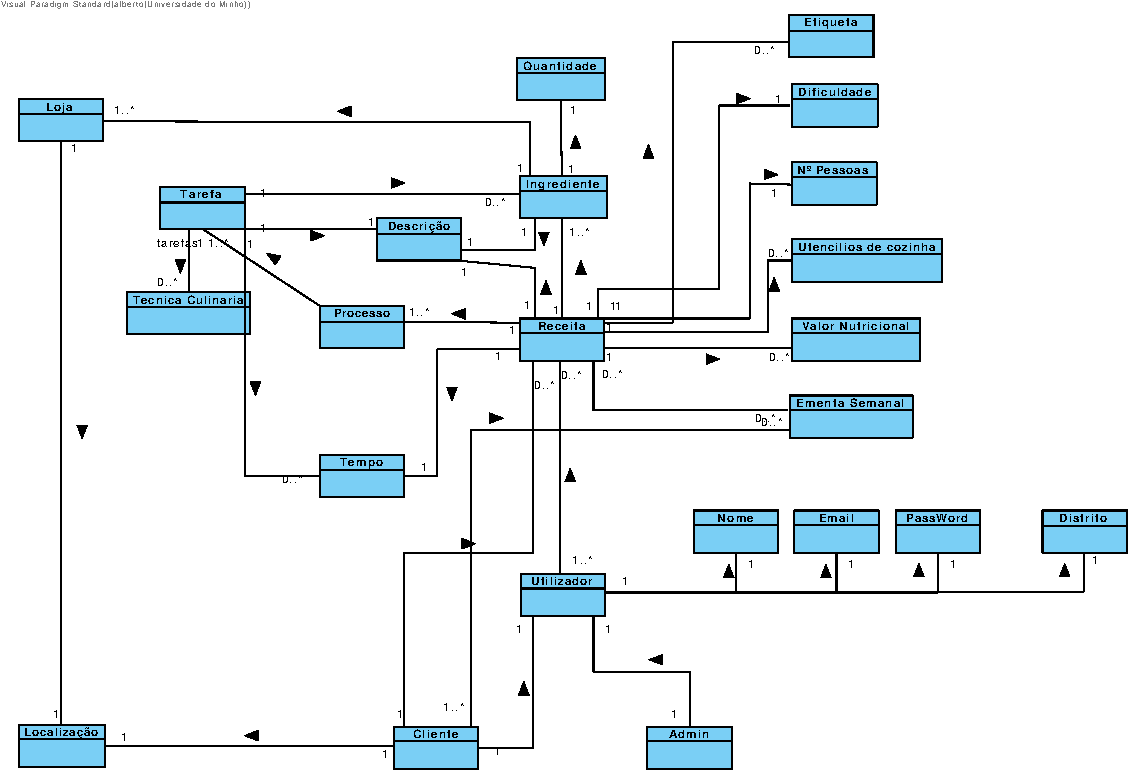
\includegraphics[width=\textwidth]{figures/04/diagrama-dominio.pdf}
  \caption{Diagrama do modelo de domínio.}
  \label{fig:dominio:diagrama}
\end{figure}

Decidiu-se que o sistema seria centrado na receita, que terá sempre uma proporção, uma dificuldade, vários ingredientes, técnicas e/ou utensílios de cozinha envolvidos, um conjunto de processos, cada um com um conjunto de tarefas que devem ser realizadas antes de prosseguir para o próximo processo, estando um tempo de execução e designação associada a cada tarefa e receita.
A receita também poderá ter valores nutricionais e etiquetas associadas a esta.

Quanto ao utilizador, este terá um nome, um email, uma palavra-passe e um distrito associado à sua conta pessoal, podendo este ser um cliente ou um administrador. Um cliente terá acesso a uma ementa semanal, com as receitas que pretende confecionar, para o almoço e jantar, nos dias de uma semana, e uma localização geográfica. 

A localização geográfica é também atribuída à loja onde o cliente poderá encontrar os diversos ingredientes usados nas receitas.

% ---------------------------------------------------------------------------- %

% Entidades:

%     - Utensílio
%     - Técnica
%     - Receita
%         - Tarefa
%             - Duração
%         - Dificuldade
%         - Quantidade de Porções
%         - Etiqueta
%         - Ingrediente
%         - Tempo de Preparação
%         - Valores Nutricionais
%     - Cliente
%         - Localização
%     - Administrador
%     - Utilizador
%         - Nome de Utilizador
%         - Palavra-Chave
%         - E-mail
%     - Histórico de Receitas Confecionadas
%     - Loja
%         - Localização
%     - Ementa Semanal

% Relacionamentos:

%     - Cliente é um Utilizador
%     - Administrador é um Utilizador

%     - Receita tem 1 Dificuldade
%     - Receita 1 tem 1..* Tarefa
%     - Receita serve 1 Quantidade de Porções
%     - Receita * é identificada por 1..* Etiqueta

%     - Cliente * tem interesse em * Etiqueta

%     - Cliente é identificado por 1 Nome de Utilizador

%     - Tarefa * faz uso de * Técnica

%     - Técnica * requer * Utensílio
%     - Passo * requer * Utensílio

% ---------------------------------------------------------------------------- %

% ---------------------------------------------------------------------------- %

\section{Levantamento e Análise de Requisitos}
\label{cap:requisitos}

Tendo-se efetuado a modelação de domínio, procedeu-se ao levantamento e análise de requisitos. Neste capítulo é primeiramente descrito o método utilizado para se efetuar a identificação de requisitos, enumerando-se de seguida os requisitos identificados. Estes utilizam o glossário definido pelo modelo concetual apresentado no capítulo anterior.

% Este documento tem como objetivo definir e especificar os requisitos necessários para o sistema \emph{Bela Sopa}, um sistema que irá integrar o sistema da cadeia de supermercados e hipermercados portuguesa \PINGODOCE.

% \emph{Bela Sopa} é um assistente pessoal baseado no serviço \emph{online} intitulado \emph{Escola de Cozinha} do \PINGODOCE, que será desenvolvido para auxiliar os seus utilizadores a cozinhar sopas, interagindo com estes durante a preparação da refeição.

% Este sistema será um incorporado pelo \PINGODOCE na sua divulgação de receitas, comercialização de produtos relacionados com estas, através de entregas ao domicílio ou na própria loja, e como publicidade para a própria empresa.

% ---------------------------------------------------------------------------- %

\subsection{Método adotado}
\label{sec:requisitos:metodo}

Durante a recolha de requisitos, recorreu-se a várias estratégias por forma a garantir que todos os requisitos necessários eram registados.

Uma vez que a nossa perceção do sistema é afetada pelas nossas experiências e gostos não é suficiente entender o que se pretende que o sistema faça, mas também adaptar o sistema aos gostos dos utilizadores por forma a encontrar um ponto de consenso e fornecer a melhor experiência possível a todos os utilizadores.

Assim para além do cliente da aplicação, o foco da nossa atenção na aquisição de requisitos são os atuais utilizadores do sistema \emph{Escola de Cozinha} e outros que constituem potenciais utilizadores, para que os requisitos sejam o mais abrangentes possíveis.

Foi assim proposto um inquérito aos utilizadores do sistema \emph{Escola de Cozinha}, para que estes partilhassem que funcionalidades extra consideravam necessárias no sistema, e analisados os dados dessa primeira plataforma de forma a obter os hábitos dos utilizadores e podermos garantir a presença e melhoria das funcionalidades mais utilizadas.

Para obter a opinião de potenciais utilizadores recorremos à partilha de questionários em plataformas de comunicação, bem como questionários presenciais em algumas das lojas da empresa \emph{Gota Doce}.

Assim da conjugação de todas as informações obtidas são extraídos os requisitos, que são posteriormente validados pela empresa cliente \emph{Gota Doce}.

% ---------------------------------------------------------------------------- %

\subsection{Requisitos levantados}
\label{sec:requisitos:levantados}

Os requisitos são divididos em \emph{requisitos de utilizador} e \emph{requisitos de sistema}, de acordo com a distinção definida por \textcite[Capítulo~4]{sommerville2010software}, para facultar uma exposição clara. São também apresentados requisitos de sistema não-funcionais.

% ---------------------------------------------------------------------------- %

\newif\ifonlyshowrequsr

% suppress missing item errors
\makeatletter
\patchcmd\endtrivlist
    {\if@newlist \@noitemerr \global\@newlistfalse \fi}
    {}
    {}{}
\patchcmd\endtrivlist
    {\@endparenv}
    {\if@newlist \@endpefalse \global\@newlistfalse \else \@endparenv \fi}
    {}{}
\makeatother

\newcommand{\labelifnotempty}[1]{%
  \if\relax\detokenize{#1}\relax \else \label{#1} \fi%
  }

\newcounter{counterrequser}

\newlist{listrequsr}{enumerate}{1}
\setlist[listrequsr]{nosep}
\setlist[listrequsr,1]{
  label=U.\arabic*.,
  ref=U.\arabic*,
  leftmargin=\widthof{\quad U.99.},
  before=\setcounter{listrequsri}{\value{counterrequser}},
  after=\setcounter{counterrequser}{\value{listrequsri}}
  }

\newlist{listreqsysfunc}{enumerate}{1}
\setlist[listreqsysfunc]{nosep}
\setlist[listreqsysfunc,1]{
  label=SF.\arabic{counterrequser}.\arabic*.,
  ref=SF.\arabic{counterrequser}.\arabic*,
  leftmargin=\widthof{\quad SF.99.9.},
  before=\setcounter{listrequsri}{\value{counterrequser}},
  after=\setcounter{counterrequser}{\value{listrequsri}}
  }

\newlist{requisitosnaofuncionais}{enumerate}{1}
\setlist[requisitosnaofuncionais]{nosep}
\setlist[requisitosnaofuncionais,1]{
  label=SNF.\arabic*.,
  ref=SNF.\arabic*,
  leftmargin=\widthof{\quad SNF.99.}
  }

\newenvironment{requisitos}[1]{%
  \textbf{#1.}%
  \ifonlyshowrequsr%
    \begin{listrequsr}%
  \else%
  \fi%
  }{%
  \ifonlyshowrequsr%
    \end{listrequsr}%
  \else%
  \fi%
  }

\newenvironment{requsr}[2]{%
  \ifonlyshowrequsr%
    \item{} #2%
    \labelifnotempty{#1}%
  \else%
    \addtocounter{counterrequser}{1}%
    \begin{listreqsysfunc}%
  \fi%
  }{%
  \ifonlyshowrequsr%
  \else%
    \end{listreqsysfunc}%
  \fi%
  }
  
\newcommand{\reqsys}[2]{%
  \ifonlyshowrequsr%
  \else%
    \item{} #2%
    \labelifnotempty{#1}%
  \fi%
  }

\newcommand{\reqsysnf}[2]{%
  \item{} #2%
  \labelifnotempty{#1}%
  }

% ---------------------------------------------------------------------------- %


% ---------------------------------------------------------------------------- %

\subsubsection{Requisitos de utilizador}
\label{sec:requisitos:levantados:utilizador}

\onlyshowrequsrtrue
\setcounter{counterrequser}{0}
% ---------------------------------------------------------------------------- %

% REQUISITOS POR ADAPTAR:

    %NAO POR \defreqsys{reqs:estado-receita}{}{O estado atual da confeção da receita é guardado caso o utilizador saia do sistema, não cancelando a confeção da receita}
 
    %DONE \defreqsys{}{}{O sistema deve apresentar e explicar o “cozinhado” ou sugerir-lhe alguns vídeos de ajuda ou sites com informação pertinente (caso o utilizador não saiba como realizar o seu cozinhado);}
    
    %DONE \defreqsys{}{}{Em fase de preparação, o sistema deve estar preparado para redirecionar o utilizador para uma das lojas mais próximas referentes ao mesmo com todos os ingredientes necessários para a confeção da sopa ou disponibilizar o serviço de entrega ao domicilio(O utilizador pode alterar estes ingredientes posteriormente).}
    
    %DONE \defreqsys{}{}{Sistema deve ser capaz de recomeçar a explicação do processo, ou voltar a explicar um processo prévio caso preciso.}
    
    %DONE \defreqsys{}{}{Um processo deverá ser capaz de conter um temporizador para a fase em questão.}
    
    %NAO POR \defreqsys{}{}{Inicialmente o sistema deve apresentar os receitas com o maior número de consultas e as receitas com a melhor classificação.}
    
% MAIS REQUISITOS POR ADAPTAR:

    %NAO POR \item Inicialmente o sistema deve apresentar os receitas mais consultadas e as receitas com a melhor classificação.
    %DONE \item Depois de uma encomenda feita o sistema abre uma nova janela.
    %DONE \item Depois de um pedido de entrega ao domicilio o sistema redireciona o cliente para a janela de preparação da sopa.
    %DONE \item Permite a um utilizador fazer login através de email e password.
    %DONE \item Permite a um utilizador se registar, fornecendo o email, nome e password e distrito.
    %DONE \item Na ementa semanal são permitidas x sopas por refeição, 2 refeições por dia, 7 dias por semana.
    %DONE \item Deve ser capaz de apresentar as configurações relativas á conta do cliente, o seu perfil, histórico de receitas já realizadas e receitas favoritas. Deve mostrar estas receitas por nome ou etiqueta.
    %DONE \item O sistema deve permitir que o utilizador mude qualquer dado da sua respectiva conta.
    
    
    
    %DONE \item Possuir um interface bastante amigável,suportado por um gestor de diálogos sofisticados e capaz de sustentar uma “conversa” razoável com o utilizador ao longo de todos os processos de trabalho, sendo capaz de especificar o passo em que se encontra e quais os passos realizados.
    %DONE\item O sistema deve permitir aos seus utilizadores definir uma configuração inicial para o sistema, deixando-os escolher aquilo que usualmente pretendem cozinhar e o tipo de ingredientes que querem usar;
    %DONE     \begin{itemize}
    %DONE         \item É possível pré-definir o que se pretende cozinhar por etiquetas.
    %DONE     \end{itemize}
    %DONE \item O sistema deve apresentar os seus serviços e funcionalidades, explicando previamente o seu modo e princípios de funcionamento;
    %DONE \item O sistema permite recordar quais as receitas favoritas de um utilizador, sendo possível adicionar ou remover desta lista nas seguintes circunstancias:
    %DONE     \begin{enumerate}
    %DONE         \item No final da confeção de uma receita;
    %DONE         \item Na vista geral de uma receita.
    %DONE     \end{enumerate}
    %DONE \item As unidades utilizadas nos ingredientes da sopa são medidos com valores concretos e em alguns casos outras unidades equivalentes.

% ---------------------------------------------------------------------------- %

\begin{requisitos}{Tipos de utilizador, contas de utilizador e autenticação}

  \begin{requsr}{}{O sistema deverá suportar dois tipos de utilizador: (1) \emph{clientes} --- o público-alvo do sistema --- e (2) \emph{administradores} --- utilizadores responsáveis pela gestão da informação disponibilizada pelo sistema.}
  
    \reqsys{}{A cada utilizador é atribuída apenas uma \emph{conta de utilizador}.}
    
    \reqsys{}{Cada conta de utilizador é classificada como \emph{de administrador} ou \emph{de cliente}, correspondendo ao tipo de utilizador homónimo, sendo identificada por um nome de utilizador e salvaguardada por meio de uma palavra-chave.}
    
    \reqsys{}{Para utilizar o sistema, um utilizador deverá primeiro autenticar-se no mesmo indicando o nome de utilizador e a palavra-chave da sua conta.}
  
    \reqsys{}{Deve sempre existir, no mínimo, uma conta de administrador.}
  
    \reqsys{}{Um utilizador não autenticado pode criar contas de cliente, fornecendo um nome de utilizador, uma palavra-chave e, opcionalmente, um email.}
    
    \reqsys{}{Um utilizador autenticado pode revogar a sua autenticação.}
  
    \reqsys{}{Um administrador autenticado pode criar e eliminar contas de administrador.}
  
    \reqsys{}{Um administrador autenticado pode eliminar contas de cliente.}
  
    \reqsys{}{Um cliente autenticado pode eliminar a sua própria conta.}
  
  \end{requsr}
  

  \begin{requsr}{}{Ao administrador é permitido a adição ou remoção de receitas do sistema.}
    
    \reqsys{}{O administrador pode adicionar uma receita nova ao sistema, a qualquer momento, fornecendo todos os elementos constituintes da mesma.}
    
    \reqsys{}{O administrador pode remover qualquer receita existente no sistema, bastando para tal especificar o identificador da mesma.}
    
    \reqsys{}{Não é permitida a existência de duas receitas com o mesmo identificador}
    
  \end{requsr}
  
  \begin{requsr}{}{O utilizador pode alterar/remover informações da sua conta.}
    
    \reqsys{}{Toda a informação armazenada em associação à conta de um utilizador, pode ser modificada pelo mesmo, excetuando informações que seja utilizadas para efeitos de identificação da conta.}
    
    \reqsys{}{Quaisquer informações opcionais, introduzidas pelo utilizador, podem ser removidas pelo mesmo}
    
  \end{requsr}

\end{requisitos}

% ---------------------------------------------------------------------------- %

\begin{requisitos}{Requisitos de execução da confeção}

  \begin{requsr}{}{No inicio da confeção, o utilizador pode confirmar que possui todos os ingredientes para a receita.}
  
    \reqsys{}{O sistema deverá apresentar, em cada receita, uma breve descrição, imagens, número de doses, quais os utensílios e ingredientes necessários e as suas respetivas quantidades, passos da receita, tempo de confeção, dificuldade, etiquetas e uma breve informação nutricional.}
    
    \reqsys{}{Caso o utilizador não tenha todos os ingredientes, este pode ser redirecionado para um serviço em que seja possível a compra / encomenda dos ingredientes.}
    
  \end{requsr}

  \begin{requsr}{}{O utilizador pode recomeçar um processo quando quiser, pode ainda voltar para um processo anterior ou avançar para o próximo, caso exista.}
  
    \reqsys{}{Cada processo deve possuir uma ou mais tarefas que são independentes entre elas.}
    
    \reqsys{}{Só é permitido avançar para o próximo processo quanto todas as tarefas, do processo atual, forem concluídas, caso não haja mais processos a execução da receita termina.}
    
    \reqsys{}{Sistema deve ser capaz de recomeçar a explicação do processo atual, ou voltar a explicar um processo prévio caso seja requerido.}
    
  \end{requsr}

  \begin{requsr}{}{Em qualquer processo da confeção da receita, em caso de dúvida o utilizador pode pedir informações ao sistema, tais como: (1) o utilizador pode pedir informação extra das técnicas de utensílio e/ou materiais no processo especifico; (2) clarificar certos termos, mostrando sinónimos a um termo; (3) quanto tempo demora o processo.}
  
    \reqsys{}{O sistema deve apresentar e explicar a receita e, caso o utilizador não saiba como concluir alguma tarefa, sugerir alguns vídeos de ajuda ou \emph{websites} com informação pertinente.}
  
    \reqsys{}{O sistema deve mostrar a lista de ingredientes, utensílios e técnicas de cozinha que são utilizados na execução da receita.}
    
    \reqsys{}{As unidades utilizadas nos ingredientes são medidos com valores concretos e em alguns casos outras unidades equivalentes.}
    
    \reqsys{}{O sistema pode mostrar a duração que cada tarefa tem, em média, e consequentemente, pode também mostrar a duração do processo.}
    
    \reqsys{}{O sistema deve permitir a alteração das palavras técnicas por outras fornecidas pelo utilizador para simplificar os processos.}
    
    \reqsys{}{Em fase de preparação, o sistema deve estar preparado para redirecionar o utilizador para uma das lojas mais próximas referentes ao mesmo com todos os ingredientes necessários para a confeção da sopa ou disponibilizar o serviço de entrega ao domicilio (O utilizador pode alterar estes ingredientes posteriormente).}
    
  \end{requsr}

  \begin{requsr}{}{Durante a confeção da sopa, em caso de uma tarefa com tempo de espera, este pode ativar um temporizador do sistema.}
  
    \reqsys{}{O sistema alerta o utilizador sonoramente quando o temporizador terminar.}
    
    \reqsys{}{O temporizador deve ser apresentado em tempo real, mostrando os minutos e segundos restantes.}
    
  \end{requsr}

  \begin{requsr}{}{Após a confeção da receita, o utilizador pode classificar a dificuldade que teve na execução da mesma.}
  
    \reqsys{}{A receita confecionada é guardada num histórico.}
    
  \end{requsr}

  \begin{requsr}{}{O utilizador pode cancelar a confeção em qualquer parte da realização da mesma.}
  
    \reqsys{}{Ao cancelar a confeção é perdida qualquer informação relativa a esta.}
    
  \end{requsr}
  


\end{requisitos}

% ---------------------------------------------------------------------------- %

\begin{requisitos}{Outros}
  
    \begin{requsr}{}{O utilizador pode questionar o sistema relativamente às sua funcionalidades.}
    
        \reqsys{}{ O sistema deve apresentar os seus serviços e funcionalidades, explicando previamente o seu modo e princípios de funcionamento}
    
    \end{requsr}

  \begin{requsr}{}{O utilizador deve conseguir procurar receitas, técnicas e utensílios através do motor de busca (permitindo um acesso rápido ao que o utilizador deseja)}
  
    \reqsys{}{As receitas podem ser pesquisadas por nome ou etiqueta.}
    
    \reqsys{}{Os utensílios podem ser pesquisados por nome.}
    
    \reqsys{}{As técnicas podem ser pesquisadas por nome.}
    
  \end{requsr}

  \begin{requsr}{}{Quando requerido, o sistema deve anotar uma ementa semanal e preparar a lista dos ingredientes necessários para cada refeição, gerando quando necessário uma lista de compras geral para a semana}
  
    \reqsys{}{A ementa semanal pode ser gerada na sua totalidade no seu menu adequado.}
    
    \reqsys{}{No menu de uma receita, esta pode ser adicionada à ementa semanal nos dias e refeições escolhidas.}
    
    \reqsys{}{Só se pode adicionar uma receita por refeição, 2 refeições por dia, 7 dias por semana}
    
  \end{requsr}

  \begin{requsr}{}{Visualizar num conjunto de \emph{dashboards} (painéis de controlo) específico a um conjunto de dados relativos aos cozinhados realizados, os tempos de preparação, as dificuldades encontradas, os ingredientes utilizados, etc..}
  
    %\reqsys{}{TODO}
    
  \end{requsr}
  
  \begin{requsr}{}{O utilizador pode definir uma configuração inicial para o sistema, deixando-os escolher aquilo que usualmente pretendem cozinhar e o tipo de ingredientes que querem usar.}
  
    \reqsys{}{É possível pré-definir o que se pretende cozinhar por etiquetas}
    
    \reqsys{}{A configuração inicial pode ser editada mais tarde nas definições de conta}
    
  \end{requsr}

  \begin{requsr}{}{O utilizador pode adicionar ou remover uma receita da sua lista de favoritos.}
  
    \reqsys{}{As receitas encontradas pelos filtros usados na janela de pesquisa podem ser adicionadas da lista de favoritos, sendo possível a sua remoção da mesma.}
    
    \reqsys{}{No final da confeção de uma receita, o utilizador pode adicioná-la à lista de favoritos, sendo possível, posteriormente, a sua remoção da lista.}
    
  \end{requsr}
  
  \begin{requsr}{}{O utilizador pode definir uma configuração inicial para o sistema, indicando que tipo de receita pretende, usualmente, confecionar e o quais os ingredientes que intendem utilizar.}
  \end{requsr}
  
\end{requisitos}

% ---------------------------------------------------------------------------- %


% ---------------------------------------------------------------------------- %

\subsubsection{Requisitos de sistema}
\label{sec:requisitos:levantados:sistema}

\onlyshowrequsrfalse
\setcounter{counterrequser}{0}
% ---------------------------------------------------------------------------- %

% REQUISITOS POR ADAPTAR:

    %NAO POR \defreqsys{reqs:estado-receita}{}{O estado atual da confeção da receita é guardado caso o utilizador saia do sistema, não cancelando a confeção da receita}
 
    %DONE \defreqsys{}{}{O sistema deve apresentar e explicar o “cozinhado” ou sugerir-lhe alguns vídeos de ajuda ou sites com informação pertinente (caso o utilizador não saiba como realizar o seu cozinhado);}
    
    %DONE \defreqsys{}{}{Em fase de preparação, o sistema deve estar preparado para redirecionar o utilizador para uma das lojas mais próximas referentes ao mesmo com todos os ingredientes necessários para a confeção da sopa ou disponibilizar o serviço de entrega ao domicilio(O utilizador pode alterar estes ingredientes posteriormente).}
    
    %DONE \defreqsys{}{}{Sistema deve ser capaz de recomeçar a explicação do processo, ou voltar a explicar um processo prévio caso preciso.}
    
    %DONE \defreqsys{}{}{Um processo deverá ser capaz de conter um temporizador para a fase em questão.}
    
    %NAO POR \defreqsys{}{}{Inicialmente o sistema deve apresentar os receitas com o maior número de consultas e as receitas com a melhor classificação.}
    
% MAIS REQUISITOS POR ADAPTAR:

    %NAO POR \item Inicialmente o sistema deve apresentar os receitas mais consultadas e as receitas com a melhor classificação.
    %DONE \item Depois de uma encomenda feita o sistema abre uma nova janela.
    %DONE \item Depois de um pedido de entrega ao domicilio o sistema redireciona o cliente para a janela de preparação da sopa.
    %DONE \item Permite a um utilizador fazer login através de email e password.
    %DONE \item Permite a um utilizador se registar, fornecendo o email, nome e password e distrito.
    %DONE \item Na ementa semanal são permitidas x sopas por refeição, 2 refeições por dia, 7 dias por semana.
    %DONE \item Deve ser capaz de apresentar as configurações relativas á conta do cliente, o seu perfil, histórico de receitas já realizadas e receitas favoritas. Deve mostrar estas receitas por nome ou etiqueta.
    %DONE \item O sistema deve permitir que o utilizador mude qualquer dado da sua respectiva conta.
    
    
    
    %DONE \item Possuir um interface bastante amigável,suportado por um gestor de diálogos sofisticados e capaz de sustentar uma “conversa” razoável com o utilizador ao longo de todos os processos de trabalho, sendo capaz de especificar o passo em que se encontra e quais os passos realizados.
    %DONE\item O sistema deve permitir aos seus utilizadores definir uma configuração inicial para o sistema, deixando-os escolher aquilo que usualmente pretendem cozinhar e o tipo de ingredientes que querem usar;
    %DONE     \begin{itemize}
    %DONE         \item É possível pré-definir o que se pretende cozinhar por etiquetas.
    %DONE     \end{itemize}
    %DONE \item O sistema deve apresentar os seus serviços e funcionalidades, explicando previamente o seu modo e princípios de funcionamento;
    %DONE \item O sistema permite recordar quais as receitas favoritas de um utilizador, sendo possível adicionar ou remover desta lista nas seguintes circunstancias:
    %DONE     \begin{enumerate}
    %DONE         \item No final da confeção de uma receita;
    %DONE         \item Na vista geral de uma receita.
    %DONE     \end{enumerate}
    %DONE \item As unidades utilizadas nos ingredientes da sopa são medidos com valores concretos e em alguns casos outras unidades equivalentes.

% ---------------------------------------------------------------------------- %

\begin{requisitos}{Tipos de utilizador, contas de utilizador e autenticação}

  \begin{requsr}{}{O sistema deverá suportar dois tipos de utilizador: (1) \emph{clientes} --- o público-alvo do sistema --- e (2) \emph{administradores} --- utilizadores responsáveis pela gestão da informação disponibilizada pelo sistema.}
  
    \reqsys{}{A cada utilizador é atribuída apenas uma \emph{conta de utilizador}.}
    
    \reqsys{}{Cada conta de utilizador é classificada como \emph{de administrador} ou \emph{de cliente}, correspondendo ao tipo de utilizador homónimo, sendo identificada por um nome de utilizador e salvaguardada por meio de uma palavra-chave.}
    
    \reqsys{}{Para utilizar o sistema, um utilizador deverá primeiro autenticar-se no mesmo indicando o nome de utilizador e a palavra-chave da sua conta.}
  
    \reqsys{}{Deve sempre existir, no mínimo, uma conta de administrador.}
  
    \reqsys{}{Um utilizador não autenticado pode criar contas de cliente, fornecendo um nome de utilizador, uma palavra-chave e, opcionalmente, um email.}
    
    \reqsys{}{Um utilizador autenticado pode revogar a sua autenticação.}
  
    \reqsys{}{Um administrador autenticado pode criar e eliminar contas de administrador.}
  
    \reqsys{}{Um administrador autenticado pode eliminar contas de cliente.}
  
    \reqsys{}{Um cliente autenticado pode eliminar a sua própria conta.}
  
  \end{requsr}
  

  \begin{requsr}{}{Ao administrador é permitido a adição ou remoção de receitas do sistema.}
    
    \reqsys{}{O administrador pode adicionar uma receita nova ao sistema, a qualquer momento, fornecendo todos os elementos constituintes da mesma.}
    
    \reqsys{}{O administrador pode remover qualquer receita existente no sistema, bastando para tal especificar o identificador da mesma.}
    
    \reqsys{}{Não é permitida a existência de duas receitas com o mesmo identificador}
    
  \end{requsr}
  
  \begin{requsr}{}{O utilizador pode alterar/remover informações da sua conta.}
    
    \reqsys{}{Toda a informação armazenada em associação à conta de um utilizador, pode ser modificada pelo mesmo, excetuando informações que seja utilizadas para efeitos de identificação da conta.}
    
    \reqsys{}{Quaisquer informações opcionais, introduzidas pelo utilizador, podem ser removidas pelo mesmo}
    
  \end{requsr}

\end{requisitos}

% ---------------------------------------------------------------------------- %

\begin{requisitos}{Requisitos de execução da confeção}

  \begin{requsr}{}{No inicio da confeção, o utilizador pode confirmar que possui todos os ingredientes para a receita.}
  
    \reqsys{}{O sistema deverá apresentar, em cada receita, uma breve descrição, imagens, número de doses, quais os utensílios e ingredientes necessários e as suas respetivas quantidades, passos da receita, tempo de confeção, dificuldade, etiquetas e uma breve informação nutricional.}
    
    \reqsys{}{Caso o utilizador não tenha todos os ingredientes, este pode ser redirecionado para um serviço em que seja possível a compra / encomenda dos ingredientes.}
    
  \end{requsr}

  \begin{requsr}{}{O utilizador pode recomeçar um processo quando quiser, pode ainda voltar para um processo anterior ou avançar para o próximo, caso exista.}
  
    \reqsys{}{Cada processo deve possuir uma ou mais tarefas que são independentes entre elas.}
    
    \reqsys{}{Só é permitido avançar para o próximo processo quanto todas as tarefas, do processo atual, forem concluídas, caso não haja mais processos a execução da receita termina.}
    
    \reqsys{}{Sistema deve ser capaz de recomeçar a explicação do processo atual, ou voltar a explicar um processo prévio caso seja requerido.}
    
  \end{requsr}

  \begin{requsr}{}{Em qualquer processo da confeção da receita, em caso de dúvida o utilizador pode pedir informações ao sistema, tais como: (1) o utilizador pode pedir informação extra das técnicas de utensílio e/ou materiais no processo especifico; (2) clarificar certos termos, mostrando sinónimos a um termo; (3) quanto tempo demora o processo.}
  
    \reqsys{}{O sistema deve apresentar e explicar a receita e, caso o utilizador não saiba como concluir alguma tarefa, sugerir alguns vídeos de ajuda ou \emph{websites} com informação pertinente.}
  
    \reqsys{}{O sistema deve mostrar a lista de ingredientes, utensílios e técnicas de cozinha que são utilizados na execução da receita.}
    
    \reqsys{}{As unidades utilizadas nos ingredientes são medidos com valores concretos e em alguns casos outras unidades equivalentes.}
    
    \reqsys{}{O sistema pode mostrar a duração que cada tarefa tem, em média, e consequentemente, pode também mostrar a duração do processo.}
    
    \reqsys{}{O sistema deve permitir a alteração das palavras técnicas por outras fornecidas pelo utilizador para simplificar os processos.}
    
    \reqsys{}{Em fase de preparação, o sistema deve estar preparado para redirecionar o utilizador para uma das lojas mais próximas referentes ao mesmo com todos os ingredientes necessários para a confeção da sopa ou disponibilizar o serviço de entrega ao domicilio (O utilizador pode alterar estes ingredientes posteriormente).}
    
  \end{requsr}

  \begin{requsr}{}{Durante a confeção da sopa, em caso de uma tarefa com tempo de espera, este pode ativar um temporizador do sistema.}
  
    \reqsys{}{O sistema alerta o utilizador sonoramente quando o temporizador terminar.}
    
    \reqsys{}{O temporizador deve ser apresentado em tempo real, mostrando os minutos e segundos restantes.}
    
  \end{requsr}

  \begin{requsr}{}{Após a confeção da receita, o utilizador pode classificar a dificuldade que teve na execução da mesma.}
  
    \reqsys{}{A receita confecionada é guardada num histórico.}
    
  \end{requsr}

  \begin{requsr}{}{O utilizador pode cancelar a confeção em qualquer parte da realização da mesma.}
  
    \reqsys{}{Ao cancelar a confeção é perdida qualquer informação relativa a esta.}
    
  \end{requsr}
  


\end{requisitos}

% ---------------------------------------------------------------------------- %

\begin{requisitos}{Outros}
  
    \begin{requsr}{}{O utilizador pode questionar o sistema relativamente às sua funcionalidades.}
    
        \reqsys{}{ O sistema deve apresentar os seus serviços e funcionalidades, explicando previamente o seu modo e princípios de funcionamento}
    
    \end{requsr}

  \begin{requsr}{}{O utilizador deve conseguir procurar receitas, técnicas e utensílios através do motor de busca (permitindo um acesso rápido ao que o utilizador deseja)}
  
    \reqsys{}{As receitas podem ser pesquisadas por nome ou etiqueta.}
    
    \reqsys{}{Os utensílios podem ser pesquisados por nome.}
    
    \reqsys{}{As técnicas podem ser pesquisadas por nome.}
    
  \end{requsr}

  \begin{requsr}{}{Quando requerido, o sistema deve anotar uma ementa semanal e preparar a lista dos ingredientes necessários para cada refeição, gerando quando necessário uma lista de compras geral para a semana}
  
    \reqsys{}{A ementa semanal pode ser gerada na sua totalidade no seu menu adequado.}
    
    \reqsys{}{No menu de uma receita, esta pode ser adicionada à ementa semanal nos dias e refeições escolhidas.}
    
    \reqsys{}{Só se pode adicionar uma receita por refeição, 2 refeições por dia, 7 dias por semana}
    
  \end{requsr}

  \begin{requsr}{}{Visualizar num conjunto de \emph{dashboards} (painéis de controlo) específico a um conjunto de dados relativos aos cozinhados realizados, os tempos de preparação, as dificuldades encontradas, os ingredientes utilizados, etc..}
  
    %\reqsys{}{TODO}
    
  \end{requsr}
  
  \begin{requsr}{}{O utilizador pode definir uma configuração inicial para o sistema, deixando-os escolher aquilo que usualmente pretendem cozinhar e o tipo de ingredientes que querem usar.}
  
    \reqsys{}{É possível pré-definir o que se pretende cozinhar por etiquetas}
    
    \reqsys{}{A configuração inicial pode ser editada mais tarde nas definições de conta}
    
  \end{requsr}

  \begin{requsr}{}{O utilizador pode adicionar ou remover uma receita da sua lista de favoritos.}
  
    \reqsys{}{As receitas encontradas pelos filtros usados na janela de pesquisa podem ser adicionadas da lista de favoritos, sendo possível a sua remoção da mesma.}
    
    \reqsys{}{No final da confeção de uma receita, o utilizador pode adicioná-la à lista de favoritos, sendo possível, posteriormente, a sua remoção da lista.}
    
  \end{requsr}
  
  \begin{requsr}{}{O utilizador pode definir uma configuração inicial para o sistema, indicando que tipo de receita pretende, usualmente, confecionar e o quais os ingredientes que intendem utilizar.}
  \end{requsr}
  
\end{requisitos}

% ---------------------------------------------------------------------------- %


\textbf{Requisitos de sistema não-funcionais.}

% ---------------------------------------------------------------------------- %

\begin{requisitosnaofuncionais}

  \reqsysnf{}{O sistema deverá disponibilizar uma interface de utilizador \emph{web}, \emph{i.e.}, acessível através de um \emph{web browser}.}

  \reqsysnf{}{O sistema deverá ser desenvolvido com recurso a tecnologias \emph{Microsoft}.}
  
  \reqsysnf{}{Possuir um interface bastante amigável,suportado por um gestor de diálogos sofisticados e capaz de sustentar uma “conversa” razoável com o utilizador ao longo de todos os processos de trabalho, sendo capaz de especificar o passo em que se encontra e quais os passos realizados.}


\end{requisitosnaofuncionais}

% ---------------------------------------------------------------------------- %


% ---------------------------------------------------------------------------- %

% \subsection{Análise geral}
% \label{sec:requisitos:analise}

% ---------------------------------------------------------------------------- %

% ---------------------------------------------------------------------------- %

\section{Modelação de \emph{Use Cases}}
\label{cap:use-cases}

Uma vez terminados os processos de modelação de domínio e de levantamento de requisitos, procedeu-se à modelação de \emph{use cases}. Neste capítulo são apresentados os resultados dessa fase.

% ---------------------------------------------------------------------------- %

\subsection{Identificação dos \emph{use cases}}
\label{sec:use-cases:identificacao}

Os use cases foram identificados através da análise dos requisitos de utilizador, de forma a satisfazer todas as funcionalidades desejadas. Deste modo, os use cases identificados podem corresponder a uma ou mais funcionalidades, oferecidas pelo sistema, visto que, algumas delas correspondem a cenários alternativos de outras.

Foram subentendidos e omitidos no diagrama de use cases, use cases acessórios relativos à conta do utilizador, tais como, \emph{logout} e \emph{editar informações de conta}, por já possuírem um comportamento normalizado. Apenas foi mencionado o use case \emph{Autenticar} pelo facto dos outros use cases possuírem como pré-condição a autentificarão do utilizador, no entanto, não é apresentada a especificação deste.

% ---------------------------------------------------------------------------- %

\subsection{Especificação dos \emph{use cases}}
\label{sec:use-cases:especificacao}

Apresentam-se nesta secção alguns exemplos representativos de especificações de \emph{use cases}. As especificações completas dos restantes \emph{use cases} identificados são incluídas no \refane{ane:use-cases-spec}.

% ---------------------------------------------------------------------------- %

\begin{table}[ht]
  \centering
  \tabelausecase
  \begin{tabularx}{\textwidth}{|>{\raggedright\let\newline\\\arraybackslash\hspace{0pt}}p{2.5cm}|>{\raggedright\let\newline\\\arraybackslash\hspace{0pt}}X|>{\raggedright\let\newline\\\arraybackslash\hspace{0pt}}X|}
    \hline
    \emph{Use case}: & \multicolumn{2}{l|}{Registar conta} \\ \hline
    Pré-condição: & \multicolumn{2}{l|}{Ator não existe} \\ \hline
    Pós-condição: & \multicolumn{2}{l|}{Ator adicionado ao sistema} \\ \hline
     & \textbf{Ator} & \textbf{Sistema} \\ \hline
    \multirow[t]{4}{=}{Comportamento Normal} &  & 1. Pergunta o email, nome, distrito e palavra-chave \\ \cline{2-3}
     & 2. Fornece dados &  \\ \cline{2-3}
     &  & 3. Valida dados \\ \cline{2-3}
     &  & 4. Adiciona utente \\ \hline
    \multirow[t]{2}{=}{Comportamento Alternativo 1 [Dados inválidos] (passo 3)} &  & 3.1. Indica ao cliente que os dados são inválidos. \\ \cline{2-3}
     &  & 3.2. Volta para 1 \\ \hline
\end{tabularx}
  \caption{Especificação do \emph{use case} ``registar conta''.}
  \label{tab:uc-registar-conta}
\end{table}

% ---------------------------------------------------------------------------- %

% ---------------------------------------------------------------------------- %

\begin{table}[ht]
  \centering
  \tabelausecase
  \begin{tabularx}{\textwidth}{|>{\raggedright\let\newline\\\arraybackslash\hspace{0pt}}p{2.5cm}|>{\raggedright\let\newline\\\arraybackslash\hspace{0pt}}X|>{\raggedright\let\newline\\\arraybackslash\hspace{0pt}}X|}
    \hline
    \emph{Use case}: & \multicolumn{2}{l|}{Procurar receitas} \\ \hline
    Pré-condição: & \multicolumn{2}{l|}{Estar autenticado} \\ \hline
    Pós-condição: & \multicolumn{2}{l|}{Encontrou pelo menos uma receita} \\ \hline
     & \textbf{Ator} & \textbf{Sistema} \\ \hline
    \multirow[t]{4}{=}{Comportamento Normal} & 1. Introduz nome de uma receita &  \\ \cline{2-3}
     &  & 2. Inicia pesquisa da receita pelo nome \\ \cline{2-3}
     &  & 3. Valida pesquisa \\ \cline{2-3}
     &  & 4. Mostra receitas encontradas \\ \hline
    \multirow[t]{3}{=}{Comportamento Alternativo 1 [Ator procura receitas por tag] (passo 1)} & 1.1. Introduz uma tag &  \\ \cline{2-3}
     &  & 1.2. Inicia pesquisa de receitas pela tag \\ \cline{2-3}
     &  & 1.3. Volta ao passo 3 \\ \hline
    Exceção 1 [Nenhuma receita corresponde à pesquisa] (passo 3) &  & 3.1. Indica que nenhuma receita foi encontrada \\ \hline
\end{tabularx}
  \caption{Especificação do \emph{use case} ``procurar receitas''.}
  \label{tab:uc-procurar-receitas}
\end{table}

% ---------------------------------------------------------------------------- %

% ---------------------------------------------------------------------------- %

\begin{table}[ht]
  \centering
  \tabelausecase
  \begin{tabularx}{\textwidth}{|>{\raggedright\let\newline\\\arraybackslash\hspace{0pt}}p{2.5cm}|>{\raggedright\let\newline\\\arraybackslash\hspace{0pt}}X|>{\raggedright\let\newline\\\arraybackslash\hspace{0pt}}X|}
    \hline
    \emph{Use case}: & \multicolumn{2}{l|}{Confecionar receita} \\ \hline
    Pré-condição: & \multicolumn{2}{l|}{Estar autenticado} \\ \hline
    Pós-condição: & \multicolumn{2}{l|}{Receita confecionada} \\ \hline
     & \textbf{Ator} & \textbf{Sistema} \\ \hline
    \multirow[t]{14}{=}{Comportamento Normal} &  & 1. Pergunta se possui todos os ingredientes. \\ \cline{2-3}
     & 2. Confirma &  \\ \cline{2-3}
     &  & 3. Pergunta se possui todos os utencílios \\ \cline{2-3}
     & 4. Confirma &  \\ \cline{2-3}
     &  & 5. Recebe o primeiro processo \\ \cline{2-3}
     &  & 6. Mostra o processo atual, as tarefas neste e os ingredientes, utensílios e técnicas nas respetivas tarefas \\ \cline{2-3}
     & 7. Confirma a execução de todas as tarefas &  \\ \cline{2-3}
     & 8. Avança &  \\ \cline{2-3}
     &  & 9. Verifica próximo processo \\ \cline{2-3}
     &  & 10. Não existe mais processos \\ \cline{2-3}
     &  & 11. Guarda a conclusão da receita \\ \cline{2-3}
     &  & 12. Pergunta a opinião sobre a conceção da receita \\ \cline{2-3}
     & 13. Responde &  \\ \cline{2-3}
     &  & 14. Guarda resposta \\ \hline
    Comportamento Alternativo 1 [Existe próximo processo] (passo 10) &  & 10.1. Recebe o próximo processo e volta ao passo 6 \\ \hline
    Comportamento Alternativo 2 [Utilizador retrocede o processo] (passo 7) &  & 7.1. Recebe o processo anterior e volta ao passo 6 \\ \hline
    \multirow[t]{3}{=}{Comportamento Alternativo 3 [Processo anterior não existe] (passo 8.1)} &  & 8.1.1. Indica que não existe um processo anterior \\ \cline{2-3}
     &  & 8.1.2. Mantêm o processo atual \\ \cline{2-3}
     &  & 8.1.3. Volta ao passo 6 \\ \hline
    Comportamento Alternativo 4 [Ator não responde] (passo 13) &  & 13.1. Termina Confecionar receita \\ \hline
    \multirow[t]{2}{=}{Exceção 1 [Não confirma] (passo 2 ou 4)} &  & 2.1. Indica para voltar quando possuir tudo \\ \cline{2-3}
     &  & 2.2. Sai do serviço Confecionar receita \\ \hline
    Exceção 2 [Utilizador cancela Confecionar receita] (passo indeterminado) &  & 2.1. Sai do serviço Confecionar receita \\ \hline
\end{tabularx}
  \caption{Especificação do \emph{use case} ``confecionar receita''.}
  \label{tab:uc-confecionar-receita}
\end{table}

% ---------------------------------------------------------------------------- %


% ---------------------------------------------------------------------------- %

%  Cliente/Administrador
% - Autenticar
% - Sair
% - Consultar/Editar informação da conta.
% - Registar conta
% \guilherme{Registar conta deveria se global visto que os dados são os mesmos} - Registar conta de administrador
% - Apagar Conta.
% - Remover Conta

% - Procurar receitas
% - Consultar receita
% - Adiciona/remove receita aos favoritos.

% - Iniciar Confeção da receita
% % Acho que isto tudo faz parte do confecionar receita.
% %- Avançar/Retroceder nos processos
% %- Iniciar temporizador
% %- Parar temporizador
% %- Concluir Confeção
% %- Cancelar Confeção da receita

% - Gerar ementa semanal
% - Editar ementa semanal
% - Adicionar/remover receita à ementa semanal.
% - Gerar lista de ingredientes

% - Aceder a serviços externos (ao domicilio).

% ---------------------------------------------------------------------------- %

% Luís:
%     -Aceder a serviçoes externos;
%     -Adicionar receita favoritos;
%     -Remover receita favoritos.

% Fábio:
%     -Gerar ementa semanal;
%     -Editar ementa semanal;
%     -Registar conta administrador;

% César:
%     -Gerar lista ingredientes;
%     -Procurar receitas;
%     -Consultar receita.

% Guilherme:

%     - Consultar/Editar informação da conta.
%     - Registar conta de cliente
%     - Registar conta de administrador
%     - Apagar Conta.

% ---------------------------------------------------------------------------- %

% ---------------------------------------------------------------------------- %

\section{Prototipagem da Interface de Utilizador}
\label{cap:interface}

Antes de se proceder à modelação da arquitetura interna do sistema, construiu-se um protótipo da interface de utilizador disponibilizada pelo sistema, o qual é descrito neste capítulo.

% ---------------------------------------------------------------------------- %

Quando a aplicação é iniciada, são requisitas as credenciais, nome de utilizador e palavra-chave, para a autenticação do utilizador. É fornecida também a opção de criar uma conta pessoa. A criação de uma conta requer, para além das informações necessárias à autenticação, a confirmação da palavra-chave e opcionalmente a introdução de um endereço de \emph{email}. Estas duas funcionalidades podem ser observadas na \reffig{fig:interface:login} e \reffig{fig:interface:registar}.

\begin{figure}[H]
  \centering 
  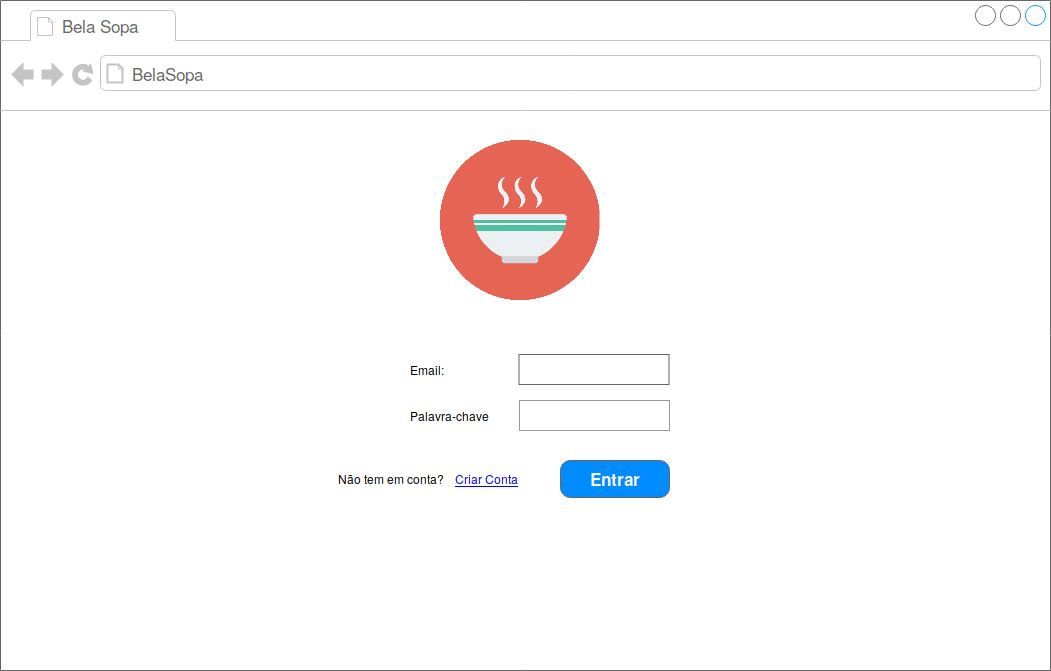
\includegraphics[width = \textwidth]{figures/07/Login.png}
  \caption{Protótipo da interface de autenticação.}
  \label{fig:interface:login}
\end{figure}

\begin{figure}[H]
  \centering 
  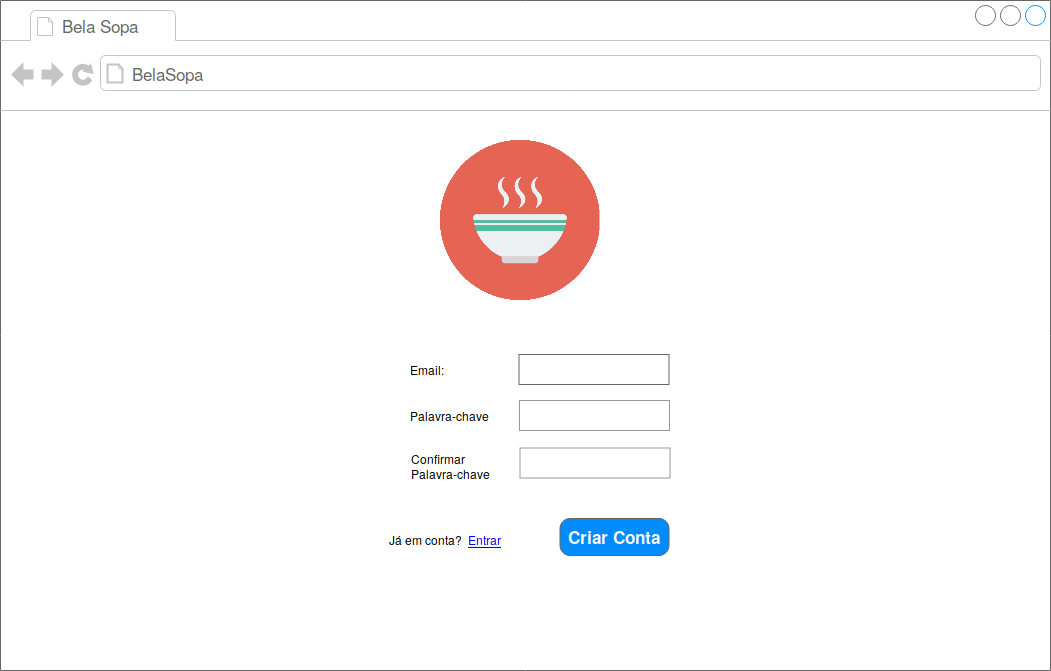
\includegraphics[width = \textwidth]{figures/07/Registar.png}
  \caption{Protótipo da interface de criação de contas.}
  \label{fig:interface:registar}
\end{figure}

Após a autenticação, é apresentado ao utilizador uma lista com todas as receitas do sistema. Nessa mesma janela é visível um menu lateral onde o utilizador pode aceder:
\begin{itemize}
    \item à sua conta pessoal;
    \item à receita que está em confeção (pode não estar visível);
    \item à lista de todas as receitas no sistema;
    \item à lista de todos os ingredientes no sistema;
    \item à lista de todas as técnicas no sistema;
    \item à lista de todos os ingredientes no sistema;
    \item à agenda semanal do utilizador;
    \item ao histórico do utilizador.
    \item à localização de lojas, \emph{Gota Doce}, próximas.
\end{itemize}
, tal como se apresenta na \reffig{fig:interface:paginicial}.

\begin{figure}[H]
  \centering 
  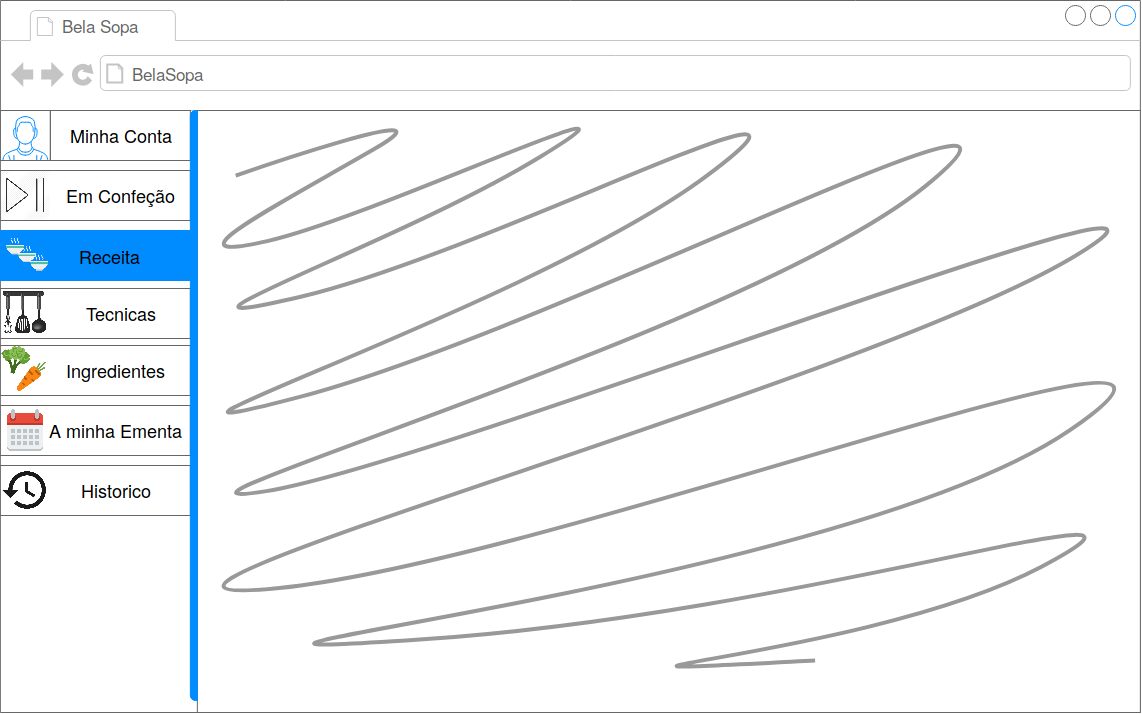
\includegraphics[width = \textwidth]{figures/07/PaginaInicial.png}
  \caption{Protótipo geral das interfaces de cliente.}
  \label{fig:interface:paginicial}
\end{figure}

A janela de pesquisa, dá a liberdade ao utilizador de pesquisar uma receita por nome, etiqueta ou por dificuldade. Depois do filtro ser ativado, são apresentadas todas as receitas que são validas de acordo com o filtro. Na apresentação das receitas, é apresentado uma imagem, titulo e etiqueta de cada receita, tal como se demonstra na \reffig{fig:interface:pesquisa}

\begin{figure}[H]
  \centering 
  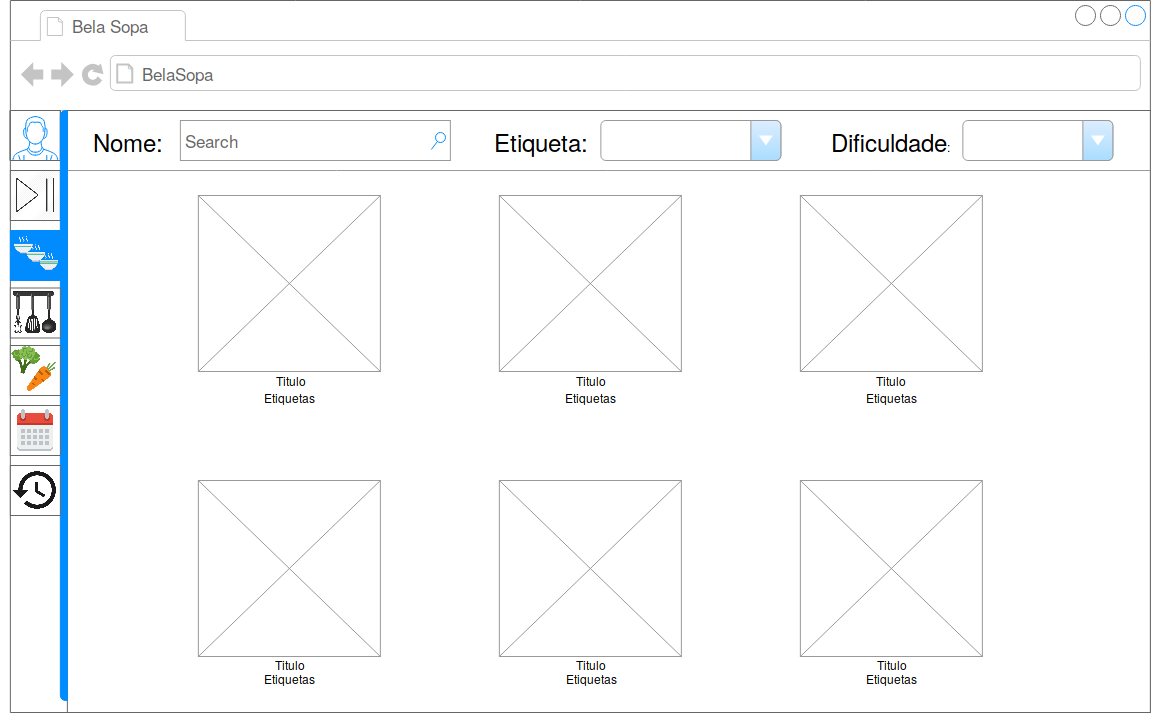
\includegraphics[width = \textwidth]{figures/07/Pesquisa.png}
  \caption{Protótipo da interface de listagem de receitas.}
  \label{fig:interface:pesquisa}
\end{figure}

Quando o utilizador seleciona uma receita, esta é apresentada como na \reffig{fig:interface:visualizacao}, ou seja, é apresentado uma imagem da receita, o titulo, uma breve descrição, a dificuldade, a etiqueta, a duração, a porção, a lista de todos os ingredientes e as suas respetivas quantidades, a lista de utensílios, a lista de técnicas, alista de tarefas e um conjunto de valores nutricionais.

\begin{figure}[H]
  \centering 
  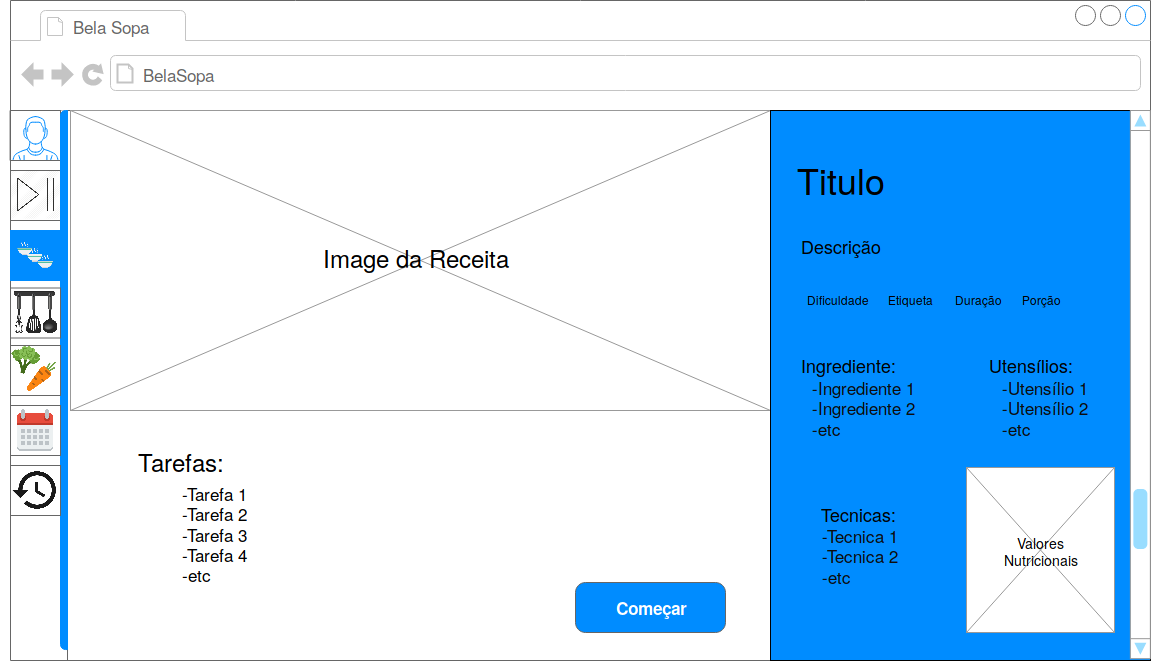
\includegraphics[width = \textwidth]{figures/07/Visualização.png}
  \caption{Protótipo da interface de visualização de uma receita.}
  \label{fig:interface:visualizacao}
\end{figure}
 
 Após iniciar a confeção, as informações da receita continuam a ser apresentados, exceto a lista de todos os ingredientes, de todos os utensílios e de todas as tarefas. Estas são reduzidas para cada processo, ou seja, em cada processo só são apresentadas as listas dos ingredientes, utensílios e tarefas referentes ao processo atual. Para alem dessas informações, a janela permite ao utilizador avançar para o processo seguinte, recuar para o processo anterior, cancelar a confeção e iniciar um temporizador, tal como demonstrado na \reffig{fig:interface:confecao}.

\begin{figure}[H]
  \centering 
  \includegraphics[width = \textwidth]{figures/07/Confeçao.png}
  \caption{Protótipo da interface de confeção de uma receita.}
  \label{fig:interface:confecao}
\end{figure}

%- Janela inicial
%    - Permite fazer login
%    - Permite registar conta de cliente

%- Janela depois de login de cliente
%    - Link para definições de conta
%    - Possibilidade de definir etiquetas pelas quais o cliente tem interesse
%    - Tab de histórico de receitas já confecionadas
%        - Incluindo dados ou estatísticas relativos aos cozinhados realizados
%    - Tab de receitas marcadas como favorito
%    - Tab de receitas
%        - Motor de busca de receitas por nome, por etiqueta
%        - Listagem de receitas por etiqueta
%    - Tab de técnicas
%        - Motor de busca de técnicas por nome
%    - Tab de configuração da ementa semanal
%        - Possibilidade de gerar lista de compras geral para uma dada semana

%- Janela de definições de conta de cliente

%    - Possibilidade de mudar passe e dados pessoais

%- Janela de receita

%    - Adicionar/remover aos/dos favoritos
%    - Adicionar à ementa semanal (especificar dia e tal)

%    - Descrição, imagens, etc.
    
%    - Porção (nº de comedores para as quantidades referidas nos passos e nos ingredientes necessários)

%    - Utensílios necessários (?)
%    - Ingredientes necessários e medidas
%    - Passos da receita
%        - Clicar no link de uma técnica no texto do passo para ver informação sobre a técnica
%    - Tempo de confeção
%    - Dificuldade
%    - Informação nutricional

%    - Link para ver Pingo Doces próximos e mostrar bing maps com percurso e tudo
%    - Link para redirecionar para loja para comprar ingredientes

%    - Começar confeção

%- Janela de confeção de receita

%    - Mesmas coisas que "janela de receita" e mais coisas
    
%    - Possibilidade de o utilizador especificar o passo em que se encontra / passos já realizados, etc.
    
%    - Os passos estão agrupados em grupos, cada grupo pode ter 1 ou mais passos, a ideia é que os passos dentro de um grupo possam ser efetuados "em paralelo", o passo atual é na verdade um grupo atual, os grupos inativos estão mais pequenos/mais cinzentos (para focar a atenção do utilizador)

% ---------------------------------------------------------------------------- %

% ---------------------------------------------------------------------------- %

\section{Arquitetura do Sistema}

Por fim, procedeu-se à modelação da arquitetura interna do sistema. Neste capítulo estabelece-se a divisão do sistema em camadas, sendo que os próximos dois capítulos detalham esta modelação.

\label{cap:arquitetura}
O sistema será dividido em três camadas principais:
\begin{enumerate}
    \item a \emph{View} que irá englobar tudo o que será necessário para a apresentação do sistema ao utilizador;
    \item o \emph{Model} que representa a camada de negócios do sistema, esta camada irá fornecer a informação necessária para a canada de apresentação;
    \item a \emph{Data} que representa os objetos de acesso à base de dados, estando cada um deles dependentes da existência do objeto respondente na camada de negócios.
\end{enumerate}

\begin{figure}[ht]
  \centering 
  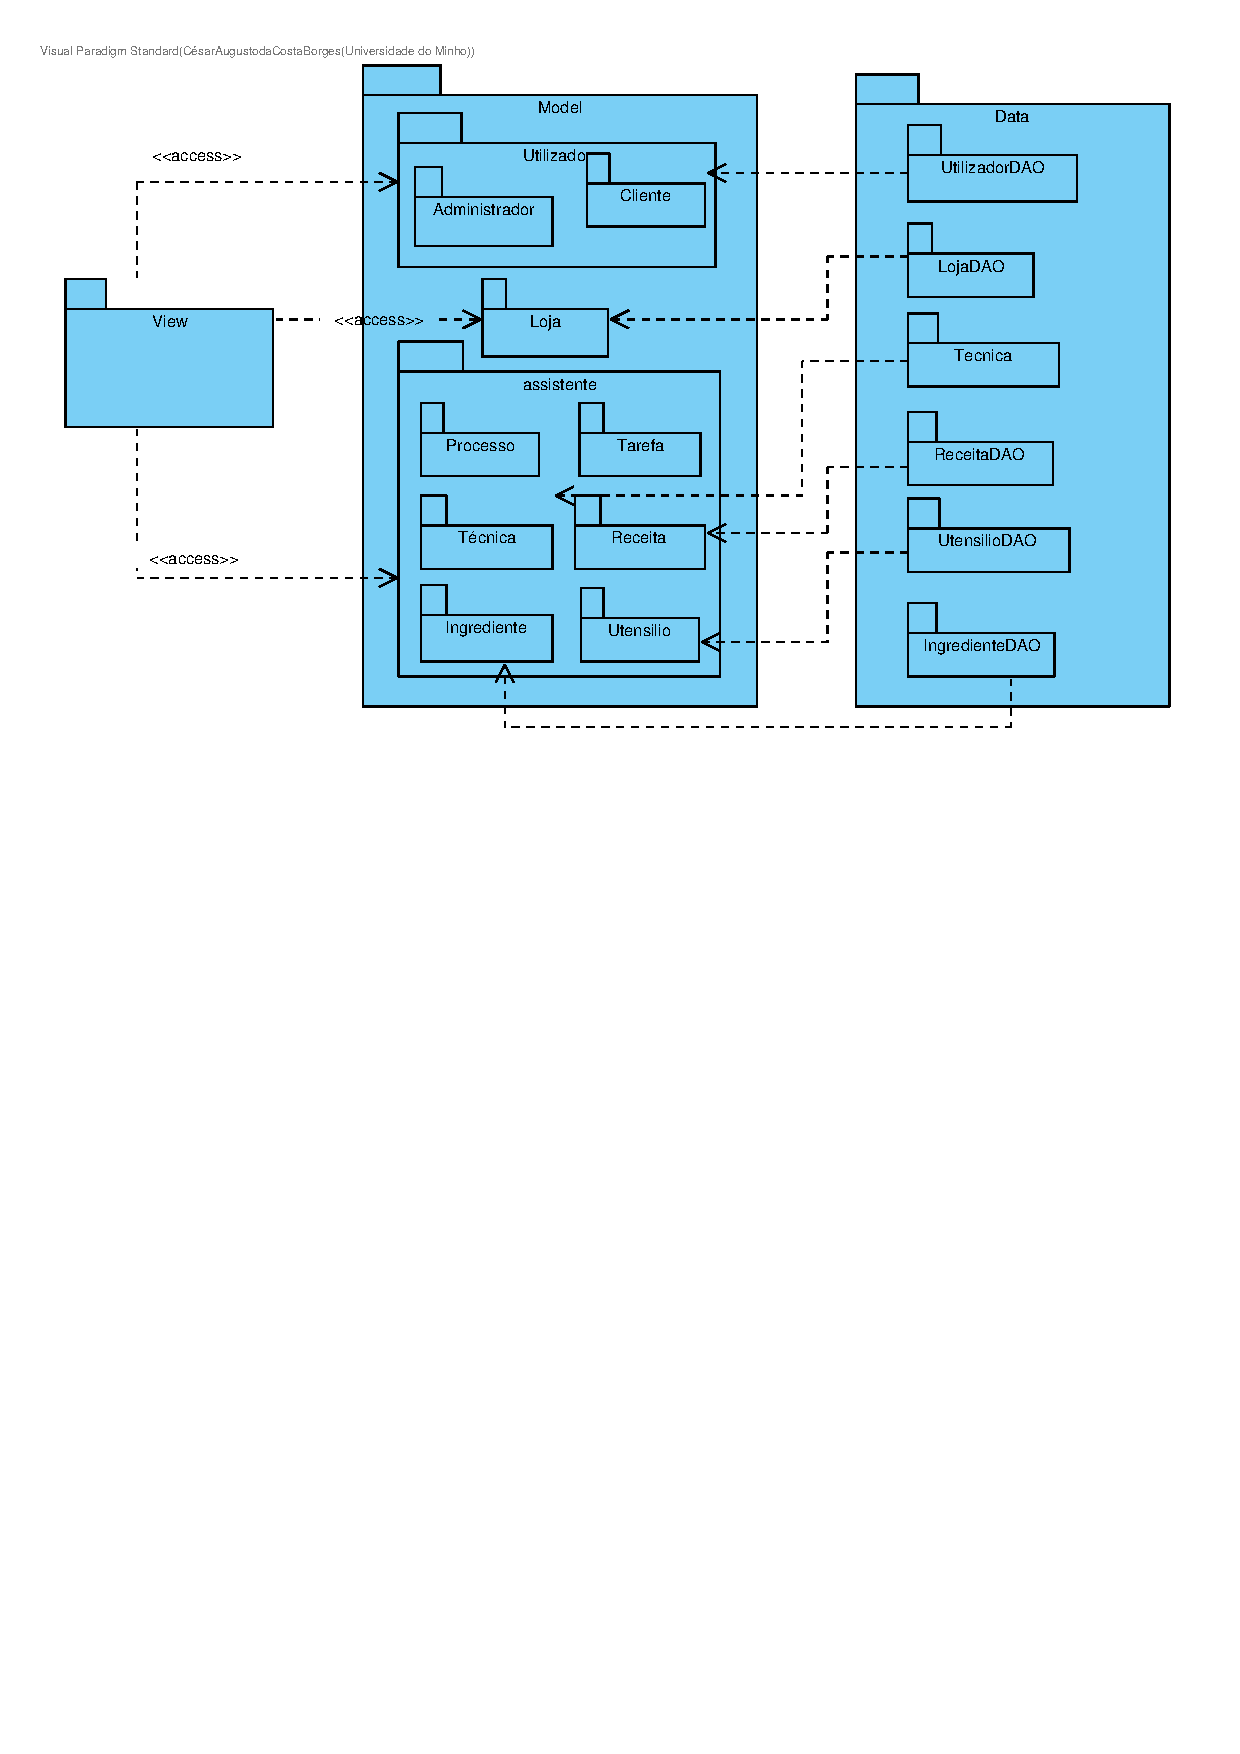
\includegraphics[width = \textwidth]{figures/08/diagrama-Pacotes.pdf}
  \caption{Diagrama de pacotes do sistema.}
  \label{fig:arquitetura:DiagramaPacotes}
\end{figure}

A camada de negócios ainda é dividida em três sub-pacotes:
\begin{enumerate}
    \item \emph{Utilizador} que está relacionado com  representação de todos os dados do utilizador;
    \item \emph{Loja} que representa os dados das lojas;
    \item \emph{Assistente} que está relacionado com o que os dados que o assistente manipulará na confeção das receitas
\end{enumerate}

%  - Arquitetura em 3 camadas
%  Relativamente à arquitetura do sistema irá ser utilizada um arquitetura em três camadas 
  
%  - Diagramas de Instalação
  
%  - Diagramas de Componentes
  
%  - (Diagramas de Pacotes)

%\begin{figure}[ht]
%  \centering
%  \includegraphics[width=\textwidth]{figures/08/pacotes.pdf}
%  \caption{Diagrama de pacotes.}
%  \label{fig:arquitetura:DiagramaPacotes}
%\end{figure}

% ---------------------------------------------------------------------------- %

% ---------------------------------------------------------------------------- %

\section{Especificação da Camada de Dados}
\label{cap:dados}

A camada de dados foi construída de modo a satisfazer a arquitetura do sistema, os requisitos funcionais mencionados anteriormente e manter a informação consistente.

% ---------------------------------------------------------------------------- %
% \subsection{Identificação de requisitos}
%\label{sec:sbd:identificacao-requisitos}
% ---------------------------------------------------------------------------- %
%\subsubsection{Abordagem adotada}
%\label{sec:sbd:identificacao-requisitos:abordagem}
% ---------------------------------------------------------------------------- %
%\subsubsection{Requisitos identificados}
%\label{sec:sbd:identificacao-requisitos:requisitos}
% ---------------------------------------------------------------------------- %
%\subsection{Modelação concetual}
%\label{sec:sbd:concetual}
%\alberto{< abordagem de modelação >}
%Administrador
%  - [PK] id      € INT
%  - email        € VARCHAR(250)
%  - palavraPasse € VARCHAR(250)
%  - nome         € VARCHAR(500)
%Cliente
%  - [PK] id      € INT
%  - email        € VARCHAR(250)
%  - palavraPasse € VARCHAR(250)
%  - nome         € VARCHAR(500)
%  - (progresso receita atual)
%Ingrediente
%Utensilio
%  - [PK] id € INT
%  - Nome    € VARCHAR(100)
%Tecnica
%  - [PK] id € INT
%
%Receita
%  - [PK] id     € INT
%  - dificuldade € { -1, 0, 1 }
%
%Tarefa
%  - [PK] id        € INT
%  - [FK] idReceita € INT
%
%ReceitaProgresso
%  - [PK, FK] idCliente € INT
%  - [FK] idReceita     € INT
%
%ReceitasConfecionadas
%  - [PK] id € INT
%  - [FK] idCliente € INT
%  - [FK] idReceita € INT
% - dataHora € DATETIME
% ---------------------------------------------------------------------------- %
%\subsubsection{Diagrama entidade-relacionamento}
%\label{sec:sbd:concetual:diagrama}
% ---------------------------------------------------------------------------- %
%\subsubsection{Validação do modelo}
%\label{sec:sbd:concetual:validacao}
% ---------------------------------------------------------------------------- %

\subsection{Diagramas de classes de objetos de acesso a dados}

Após o diagrama de classes estar bem definido e estruturado, estipularam-se as entidades a persistir.
Estas foram o \emph{Utilizador}, \emph{Cliente}, \emph{Etiqueta}, \emph{Loja}, \emph{Receita}, \emph{Técnica}, \emph{Utensílios} e \emph{Ingredientes} devido á sua importância para a consistência do sistema. Todos os dados destas classes teriam agora que ser fornecidos pela base de dados,separando assim a camada de negócio da camada de dados.
Em baixo é ilustrado diagrama de classes com as entidades persistidas, ilustradas a cinzento.
\begin{figure}[H]
  \centering
  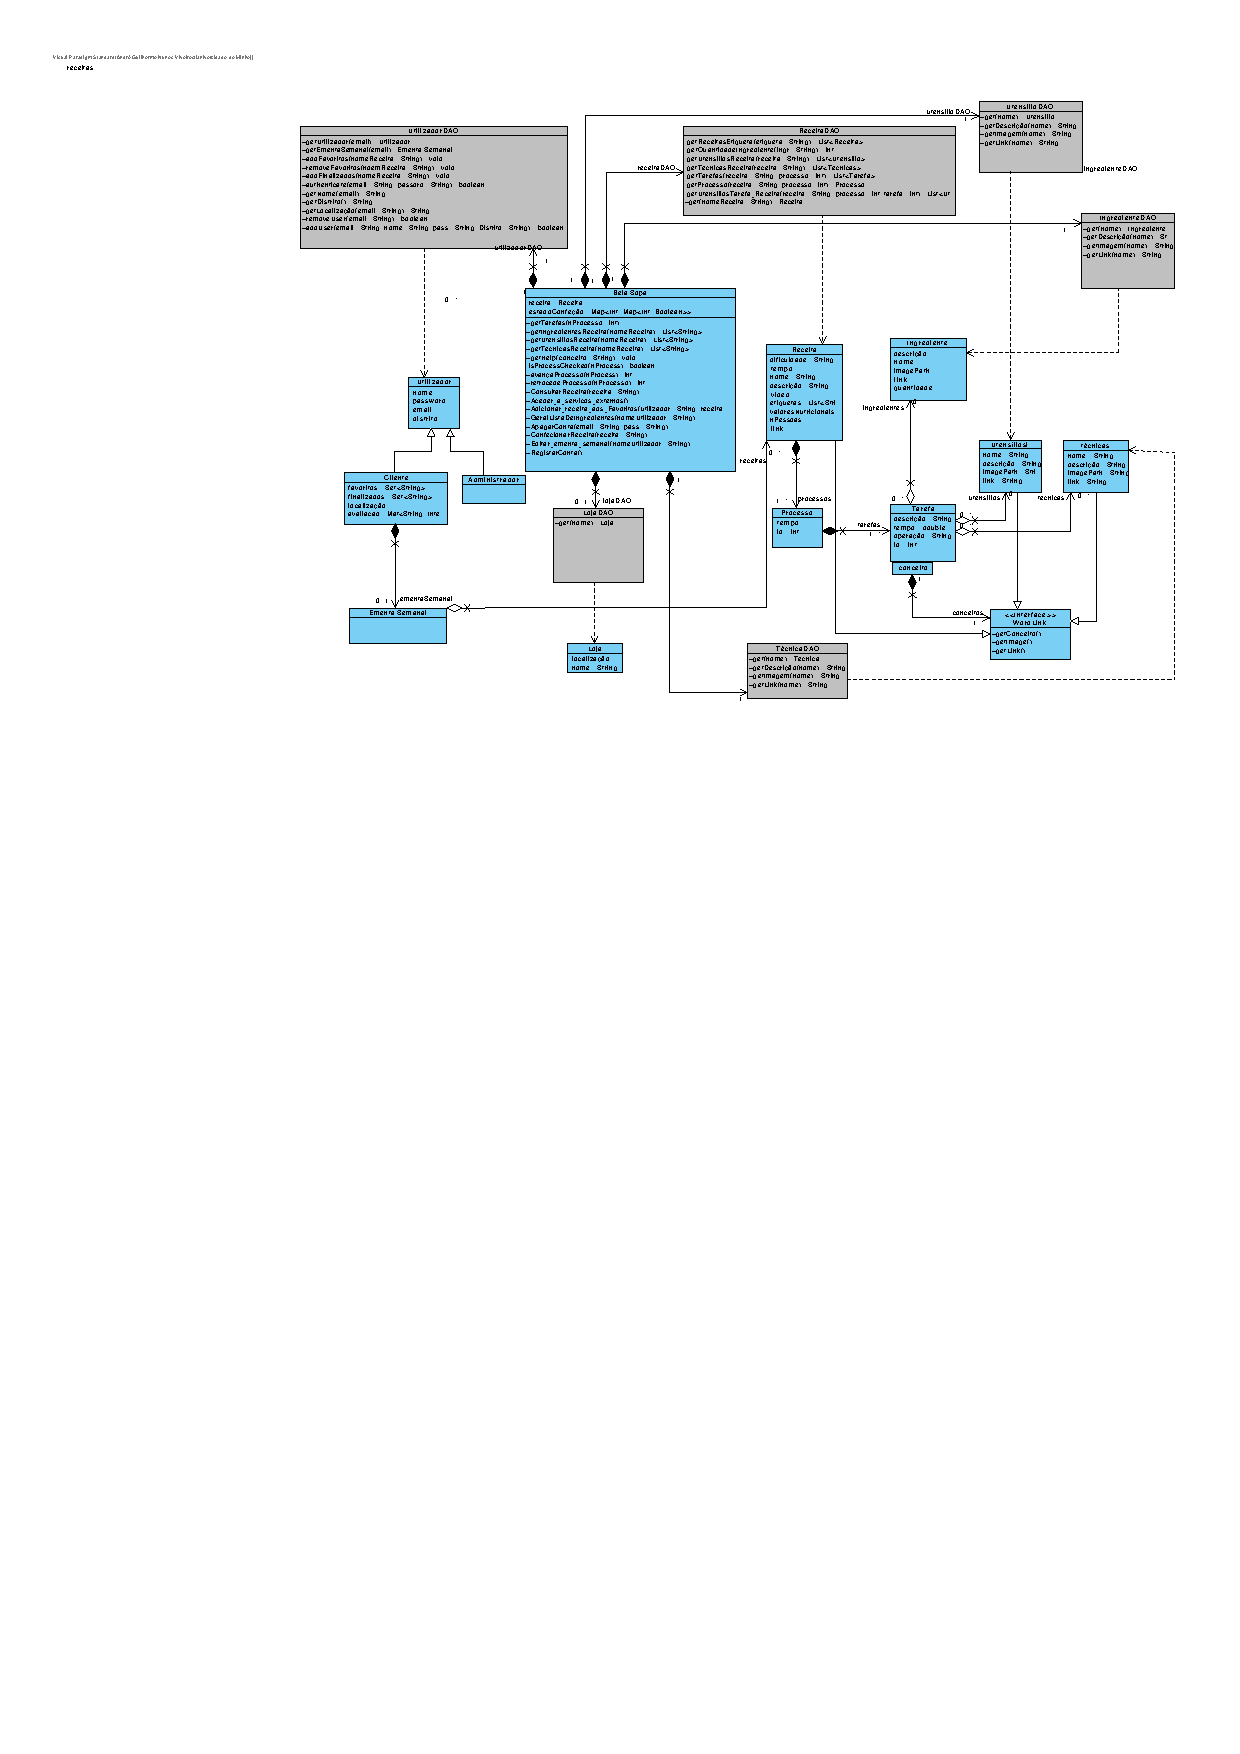
\includegraphics[width=\textwidth]{figures/09/Diagram_classe_com_DAO.pdf}
  \caption{Diagrama de classes para a camada de dados.}
\end{figure}

% ---------------------------------------------------------------------------- %

\subsection{Modelação concetual da base de dados}
\label{sec:sbd:concetual:ent-rel-atr}

Foram subentendidos no diagrama de classes apresentado anteriormente, todos as entidades a serem criadas tais como os seus respectivos atributos.
Dito isto foram estabelecidas as relações entre as entidades. Para uma compreensão mais legível das mesmas decidiu-se utilizar o modelo concetual apenas para realçar estas relações, o qual é apresentado na \reffig{fig:concetuallllll} e utiliza a notação Chen~\parencite{chen1976entity}.

\begin{figure}[ht]
  \centering
  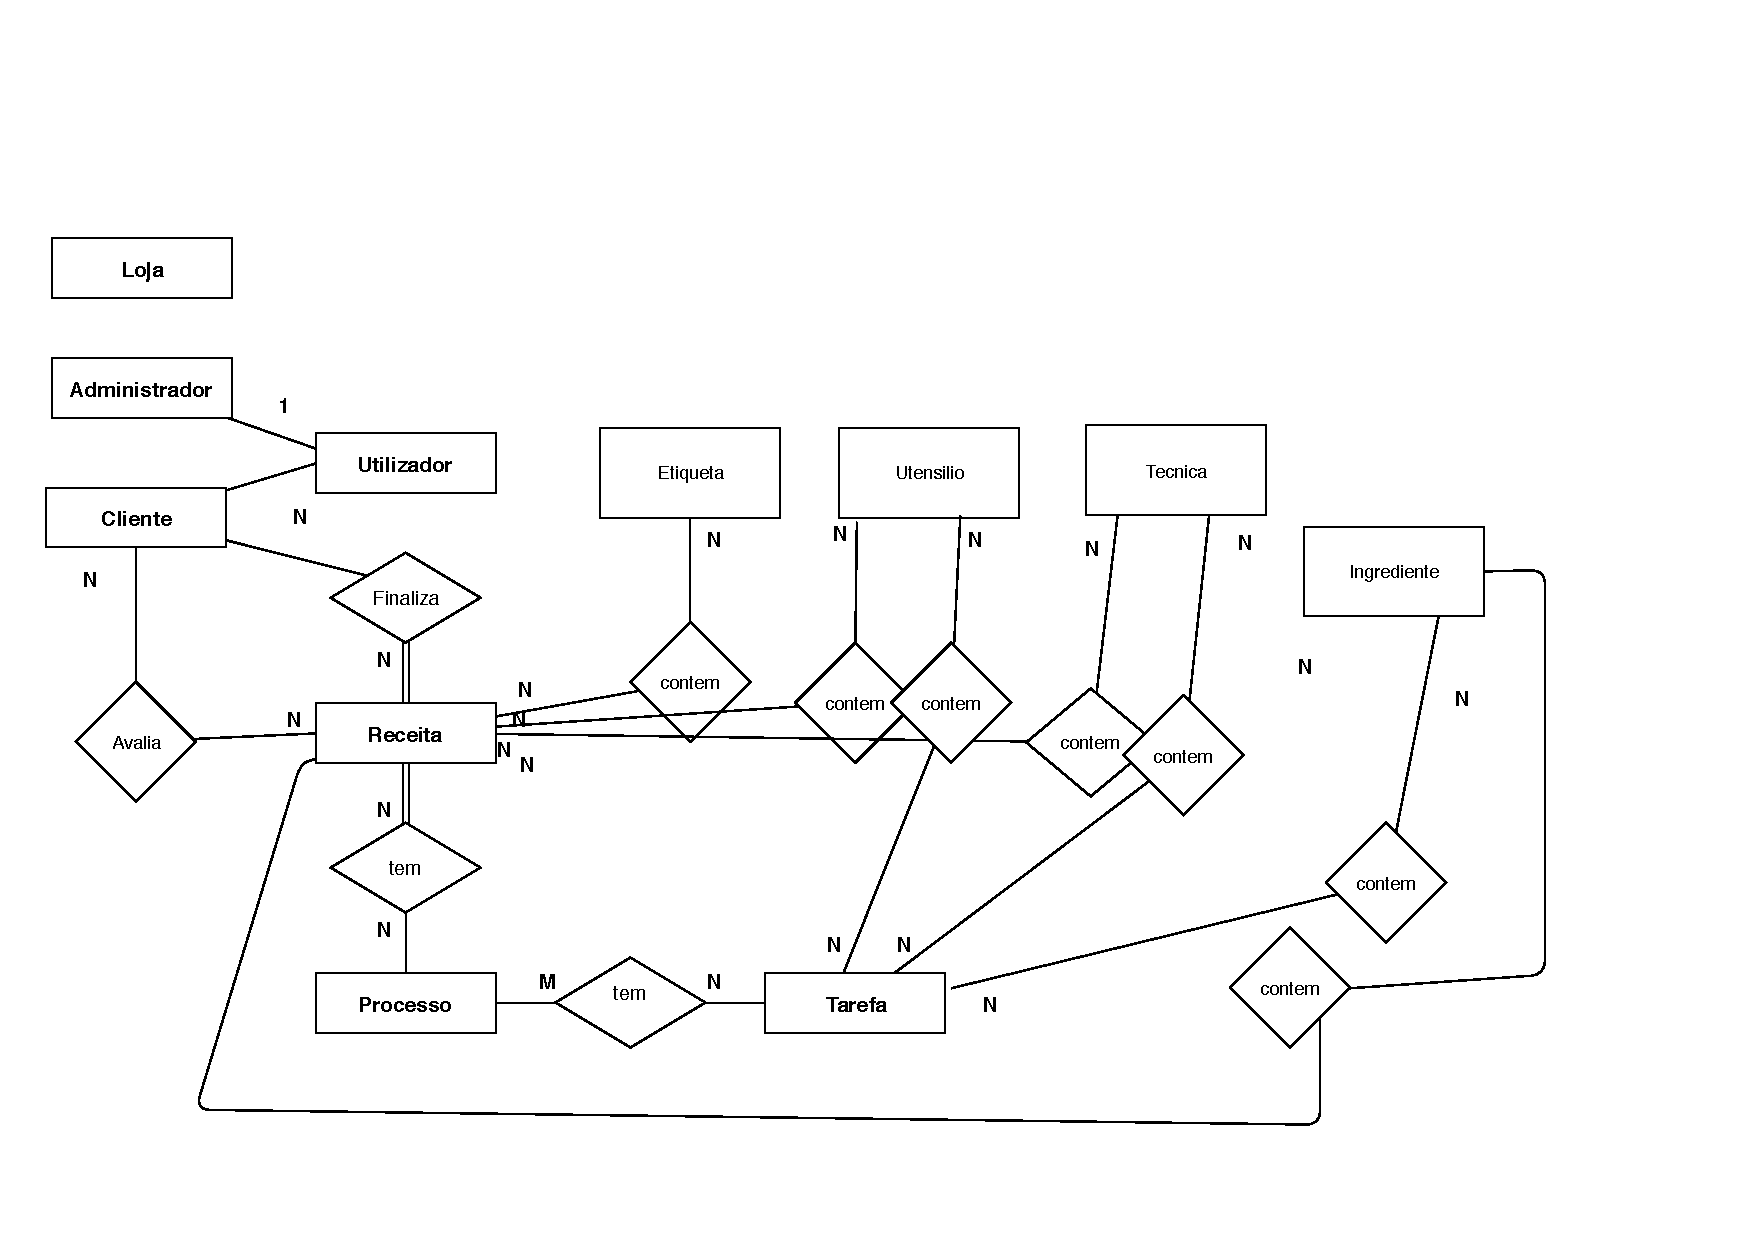
\includegraphics[width=\textwidth]{figures/09/sbd-concetual.pdf}
  \caption{Modelo concetual da base de dados.}
  \label{fig:concetuallllll}
\end{figure}

% ---------------------------------------------------------------------------- %

\subsection{Modelação lógica da base de dados}
\label{sec:sbd:logico}

Tendo as relações definidas elaborou-se o modelo lógico através do programa \emph{MySQL Workbench}\footnote{\url{https://www.mysql.com/products/workbench/}, acedido a 23 de maio de 2019}, o qual se apresenta na \reffig{fig:logicoooooooooo}.

\begin{figure}[ht]
  \centering
  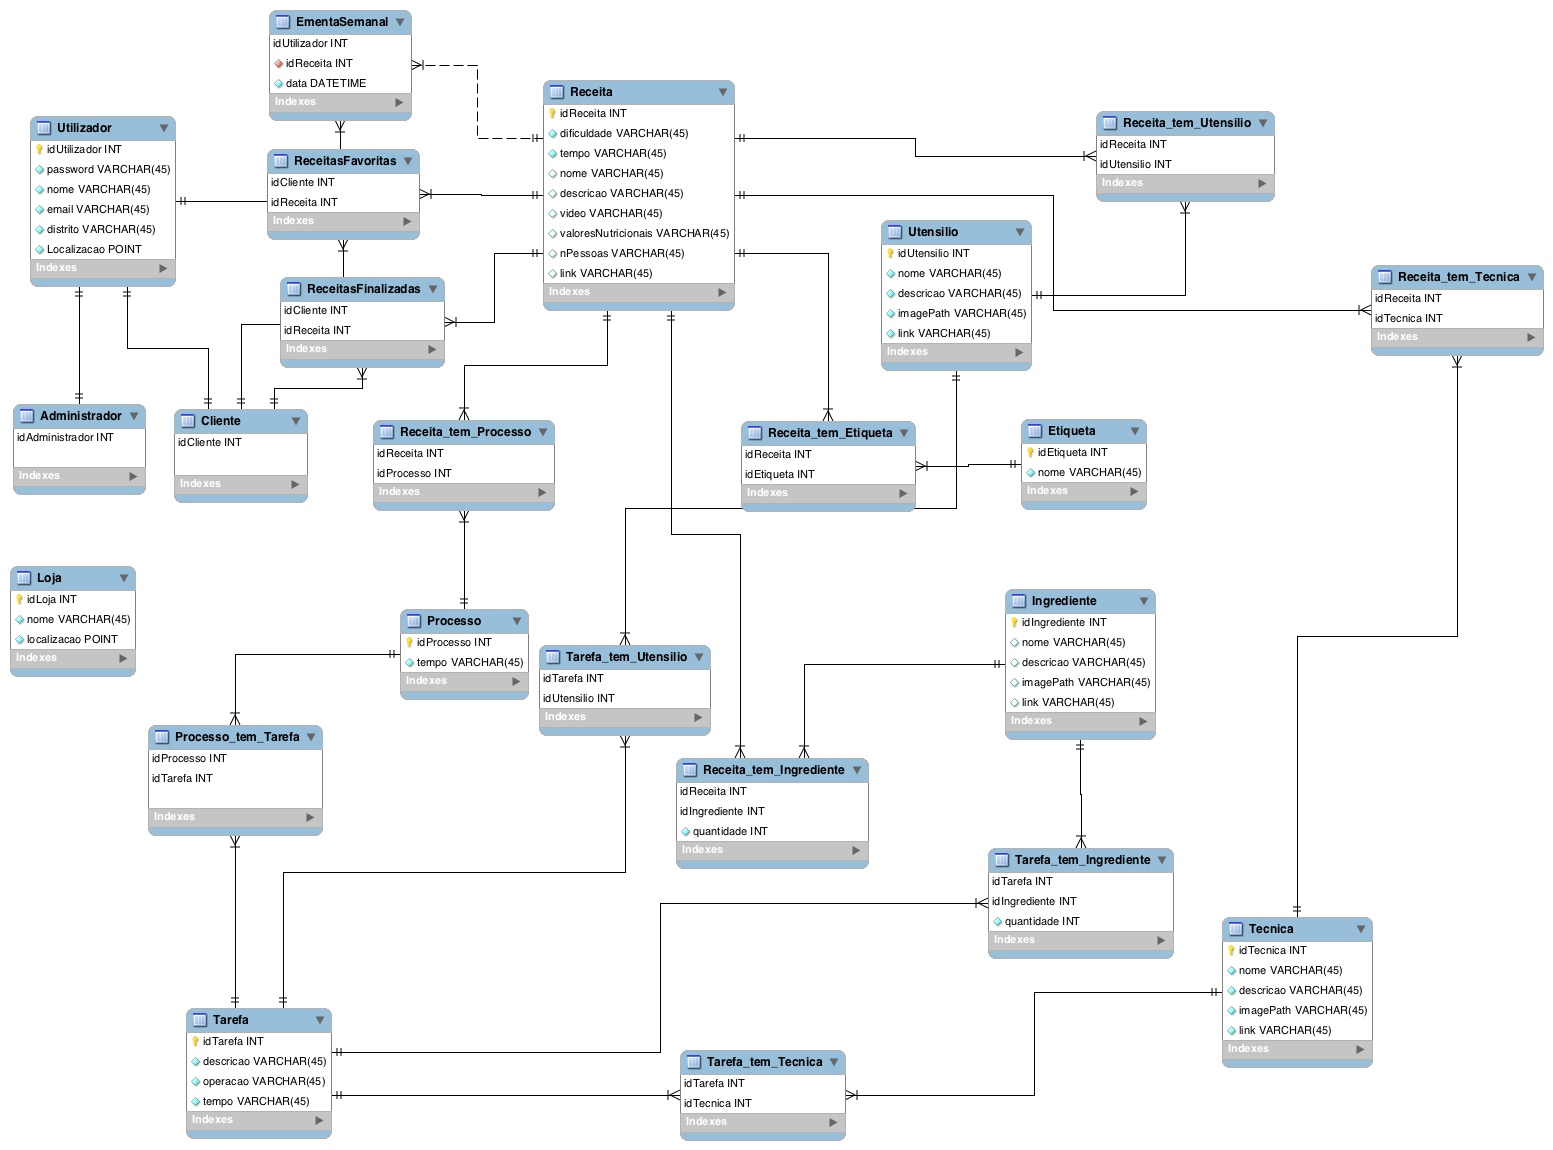
\includegraphics[width=\textwidth]{figures/09/sbd-logico.png}
  \caption{Modelo lógico da base de dados.}
  \label{fig:logicoooooooooo}
\end{figure}

% ---------------------------------------------------------------------------- %
%\subsubsection{Desenho do modelo}
%\label{sec:sbd:logico:desenho}
% ---------------------------------------------------------------------------- %
%\subsubsection{Validação do modelo}
%\label{sec:sbd:logico:validacao}
%\alberto{< através da normalização (até 3NF) >}
%\alberto{< com interrogações >}
%\alberto{< com transações >}
% ---------------------------------------------------------------------------- %

% ---------------------------------------------------------------------------- %

\section{Especificação da Camada de Negócio}
\label{cap:negocio}

A camada de negócio engloba toda a lógica interna do sistema e as suas responsabilidades passam pelo processamento dos pedidos provenientes da camada de apresentação por forma a cumprir os requisitos funcionais do sistema, bem como assegurar o cumprimento de requisitos não-funcionais.

Assim para especificar a mesma recorreu-se a um diagrama de classes que irá apresentar as diversas classes que constituem esta camada, bem como abordar de forma mais especifica todas as componentes das mesmas e diagramas de sequência que demonstram e descrevem a interação entre essas classes.

Um diagrama de pacotes onde se pode ver a estrutura genérica da camada de negócio foi já fornecido no \refcap{cap:arquitetura}, apresentado na \reffig{fig:arquitetura:DiagramaPacotes}, sendo o pacote referente à camada de negócio o \emph{Model}.

\subsection{Diagramas de classes}
\label{subsec:diagramas_classe}

O presente diagrama de classes apresenta então como classes constituintes da camada de negócio, as classes:

\begin{itemize}
    \item Bela Sopa;
    \item Utilizador;
    \item Administrador;
    \item Cliente;
    \item Localização;
    \item Ementa Semanal;
    \item Loja;
    \item Receita;
    \item Processo;
    \item Tarefa;
    \item Ingrediente;
    \item Utensílios;
    \item Técnicas.
\end{itemize}

As relações entre as entidade são também descritas no diagrama, fornecendo uma vista geral da estrutura do sistema.

 \begin{figure}[H]
   \centering
   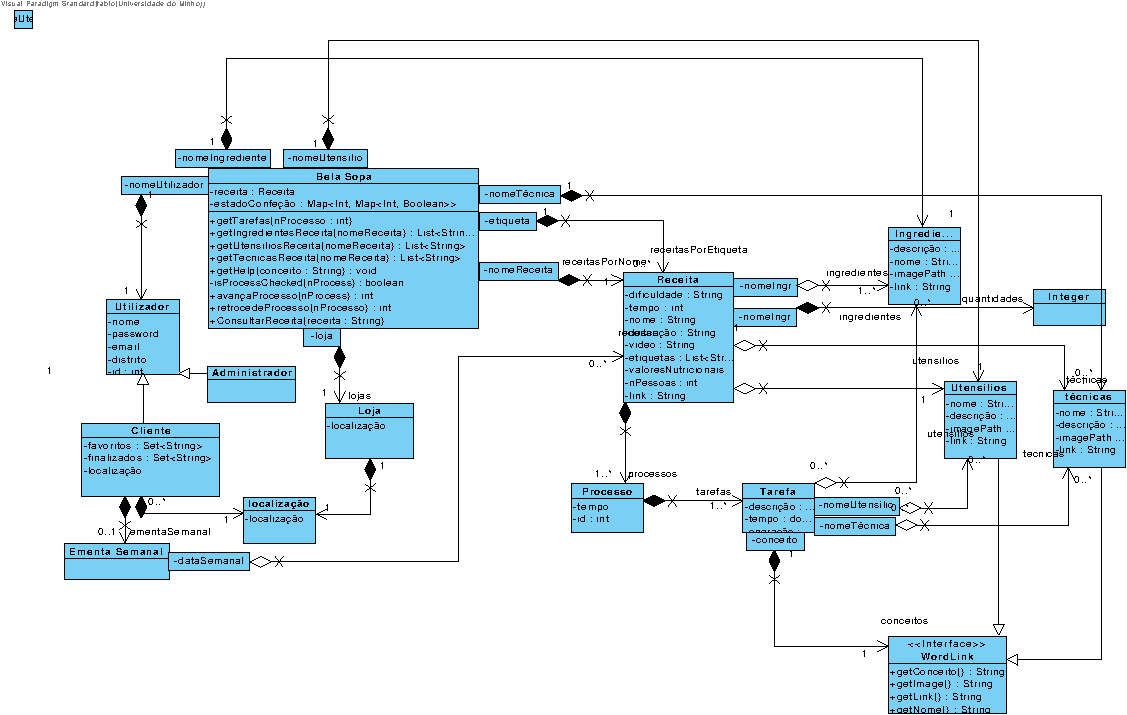
\includegraphics[width=\textwidth]{figures/10/Diagrama_Classes.pdf}
   \caption{Diagrama de classes para a camada de negócio.}
   \label{fig:negocio:DiagramaClasses}
 \end{figure}

\subsection{Diagramas de sequência}
\label{subsec:diagramas_sequencia}

Para demonstrar as classes que compõem a camada de negócio, a forma como estas se relacionam e interatuam entre si, e as suas funções, apresentam-se, a título ilustrativo, os diagramas de sequência de dois eventos do sistema:

\begin{itemize}
    \item Confecionar Receita;
    \item Consultar Receita.
\end{itemize}

\begin{figure}[H]
   \centering
   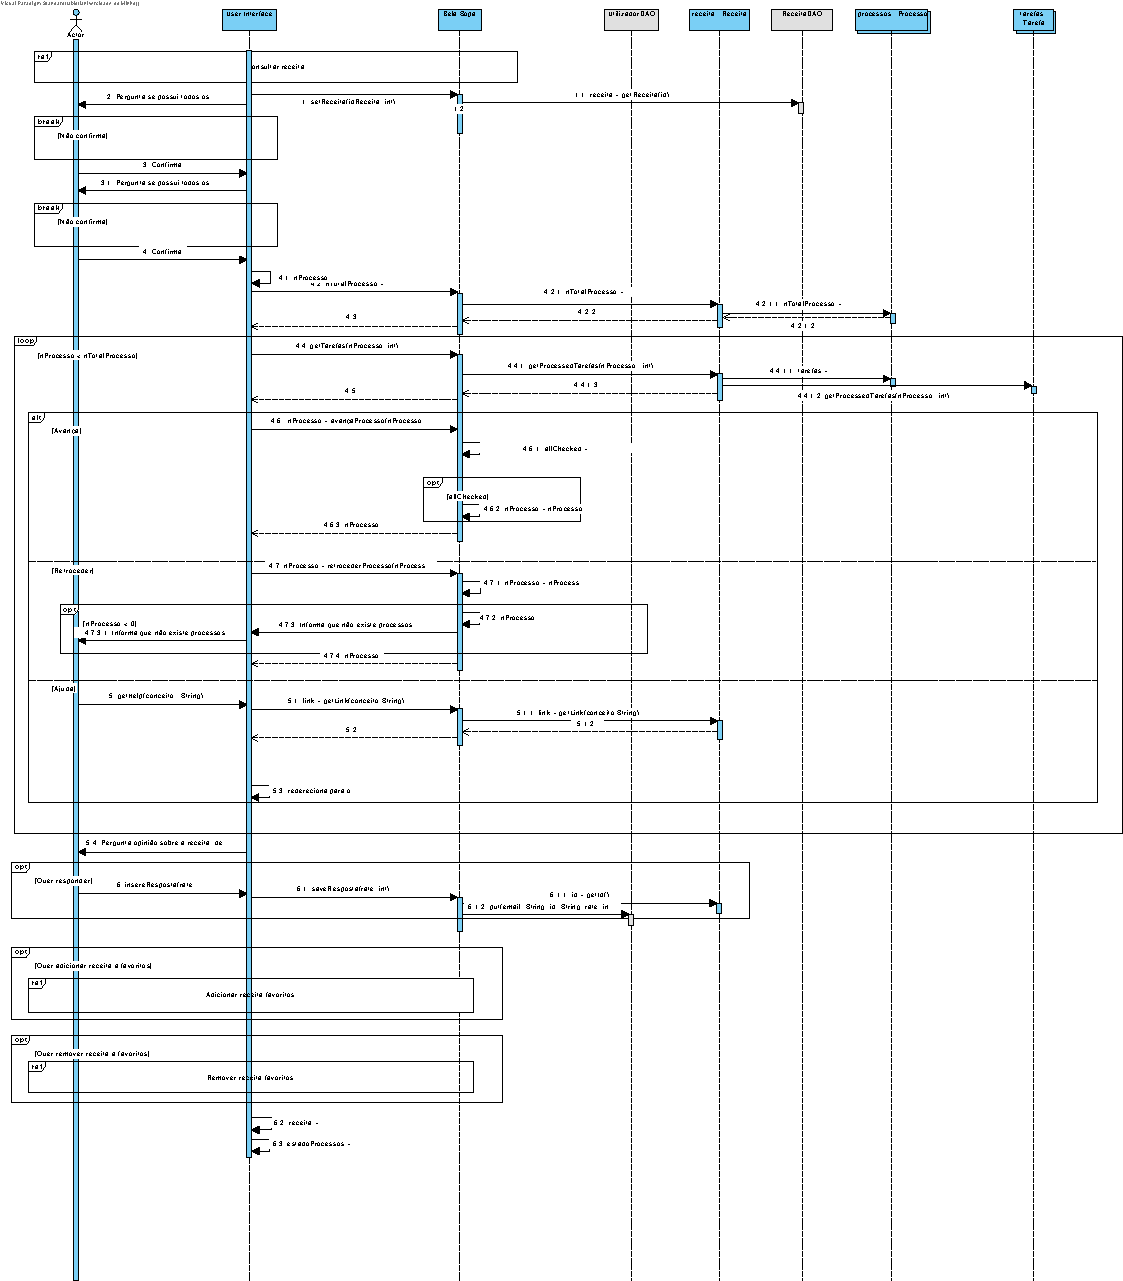
\includegraphics[width=\textwidth]{figures/10/Confecionar_receita.pdf}
   \caption{Diagrama de sequência para a confeção de uma receita.}
   \label{fig:negocio:DiagramaSequencia1}
 \end{figure}

\begin{figure}[H]
   \centering
   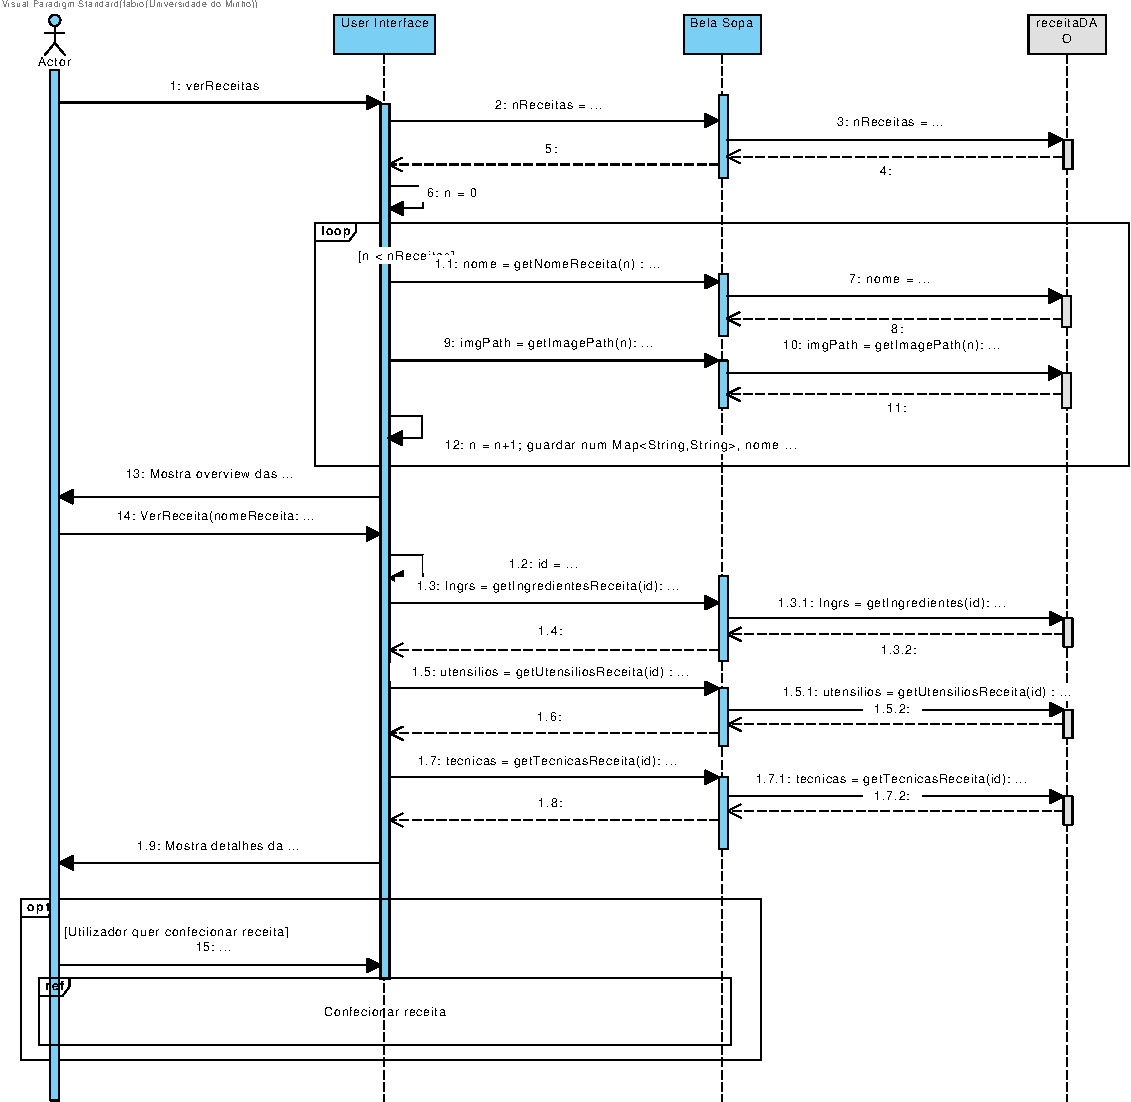
\includegraphics[width=\textwidth]{figures/10/Consultar_receita.pdf}
   \caption{Diagrama de sequência para a consulta de uma receita.}
   \label{fig:negocio:DiagramaSequencia2}
 \end{figure}
 
 Os restantes diagramas de sequência podem ser encontrados no \refane{ane:negocio-diag-seq}. 

% ---------------------------------------------------------------------------- %

% ---------------------------------------------------------------------------- %

\section{Construção}
\label{cap:construcao}

Tendo-se terminado o processo de especificação do sistema, procedeu-se à sua implementação. Neste capítulo são primeiramente enumeradas as principais tecnologias utilizadas na sua construção, descrevendo-se também vários aspetos relevantes da sua implementação. É depois descrito o procedimento de instalação do sistema e apresentado brevemente o produto obtido.

% ---------------------------------------------------------------------------- %

\subsection{Tecnologias utilizadas}
\label{sec:construcao:tecnologias}

O sistema desenvolvido consiste em um servidor \emph{web}, o qual é acedido por clientes remotos através de um \emph{web browser}. Para a implementação do mesmo, utilizaram-se as seguintes principais tecnologias e \emph{frameworks}:

\begin{itemize}

    \item Sistema de gestão de bases de dados \emph{Microsoft SQL Server}\footnote{\url{https://www.microsoft.com/en-us/sql-server}, acedido a 23 de maio de 2019};

    \item \emph{Microsoft .NET Core} 2.1\footnote{\url{https://dotnet.microsoft.com/}, acedido a 23 de maio de 2019}, utilizando-se a liguagem \emph{C\#};

    \item \emph{Entity Framework Core} 2.1\footnote{\url{https://dotnet.microsoft.com/apps/aspnet}, acedido a 23 de maio de 2019};

    \item \emph{Microsoft ASP.NET Core} 2.1\footnote{\url{https://docs.microsoft.com/en-us/ef/core}, acedido a 23 de maio de 2019}, utilizando-se a arquitetura \emph{Model-View-Controller} (MVC);
    
    \item \emph{Bing Maps API}\footnote{\url{https://www.microsoft.com/en-us/maps/choose-your-bing-maps-api}, acedido a 23 de maio de 2019};
    
    \item \emph{YamlDotNet} 6.0\footnote{\url{https://github.com/aaubry/YamlDotNet}, acedido a 23 de maio de 2019}.

\end{itemize}

% ---------------------------------------------------------------------------- %

\subsection{Detalhes de implementação}
\label{sec:construcao:implementacao}

O sistema desenvolvido segue o padrão arquitetural \emph{Model-View-Controller} (MVC):

\begin{itemize}

    \item \emph{Models}: representam, gerem e persistem a informação utilizada pelo sistema;
    
    \item \emph{Views}: definem a interface gráfica disponibilizada aos utilizadores do sistema, apresentando informação gerida pelos \emph{models};
    
    \item \emph{Controllers}: gerem a interação do utilizador com a interface gráfica disponibilizada pelas \emph{views}, interatuando com os \emph{models} para obter e modificar informação.
    
\end{itemize}

A informação da aplicação é persistida numa base de dados relacional disponibilizada por uma instância de um servidor \emph{Microsoft SQL Server}. O mapeamento do modelo relacional para objetos foi implementado com recurso à plataforma \emph{Entity Framework Core}.

% ---------------------------------------------------------------------------- %

\subsection{Procedimento de instalação}
\label{sec:construcao:instalacao}

Uma vez que o sistema desenvolvido corresponde apenas a um \emph{web} server, o processo de instalação (ou \emph{deployment}) do mesmo envolve apenas intervenção por parte do administrador da máquina onde se deseja que este corra.

Por forma a se instalar o sistema, os seguintes pré-requisitos devem ser cumpridos:

\begin{itemize}

    \item A máquina onde o \emph{web} server irá correr deve utilizar alguma versão do sistema operativo \emph{Windows} com suporte para as tecnologias enumeradas na secção anterior;
    
    \item A mesma máquina deve ter acesso (local ou remoto) a uma instância de um servido \emph{Microsoft SQL Server}, no qual os dados da aplicação serão persistidos.
    
\end{itemize}

Tendo em conta que a aplicação é disponibilizada num único arquivo de ficheiros, o procedimento de instalação do sistema consiste então nos seguintes passos:

\begin{enumerate}

    \item Extrair todo os ficheiros do arquivo da aplicação;

    \item Alterar o campo \path{ConnectionStrings.DefaultConnection} do ficheiro \path{appsettings.json} por forma a corresponder à instância do servidor \emph{Microsoft SQL Server} (e base de dados nesse servidor) onde os dados da aplicação devem ser persistidos;
    
    \item Executar o programa \path{BelaSopa.exe}, o qual corresponde ao servidor \emph{web} que implementa o sistema;
    
    \item Opcionalmente, configurar o sistema operativo por forma a que este programa seja executado aquando do reinício da máquina;

    \item Garantir que eventuais configurações de rede permitam que clientes remotos acedam ao servidor \emph{web}.
    
\end{enumerate}

Uma vez concluído este processo, os clientes terão acesso ao sistema através do seu \emph{web browser}, especificando o endereço da máquina em que o servidor \emph{web} está instalado.

% ---------------------------------------------------------------------------- %

\subsection{Produto final}
\label{sec:construcao:produto-final}

As Figuras~\ref{fig:construcao:final-1} a~\ref{fig:construcao:final-4} apresentam, a título de exemplo, o aspeto final de várias interfaces representativas disponibilizadas pelo sistema \emph{Bela Sopa}.

\begin{landscape}

\begin{figure}[p]
  \centering
  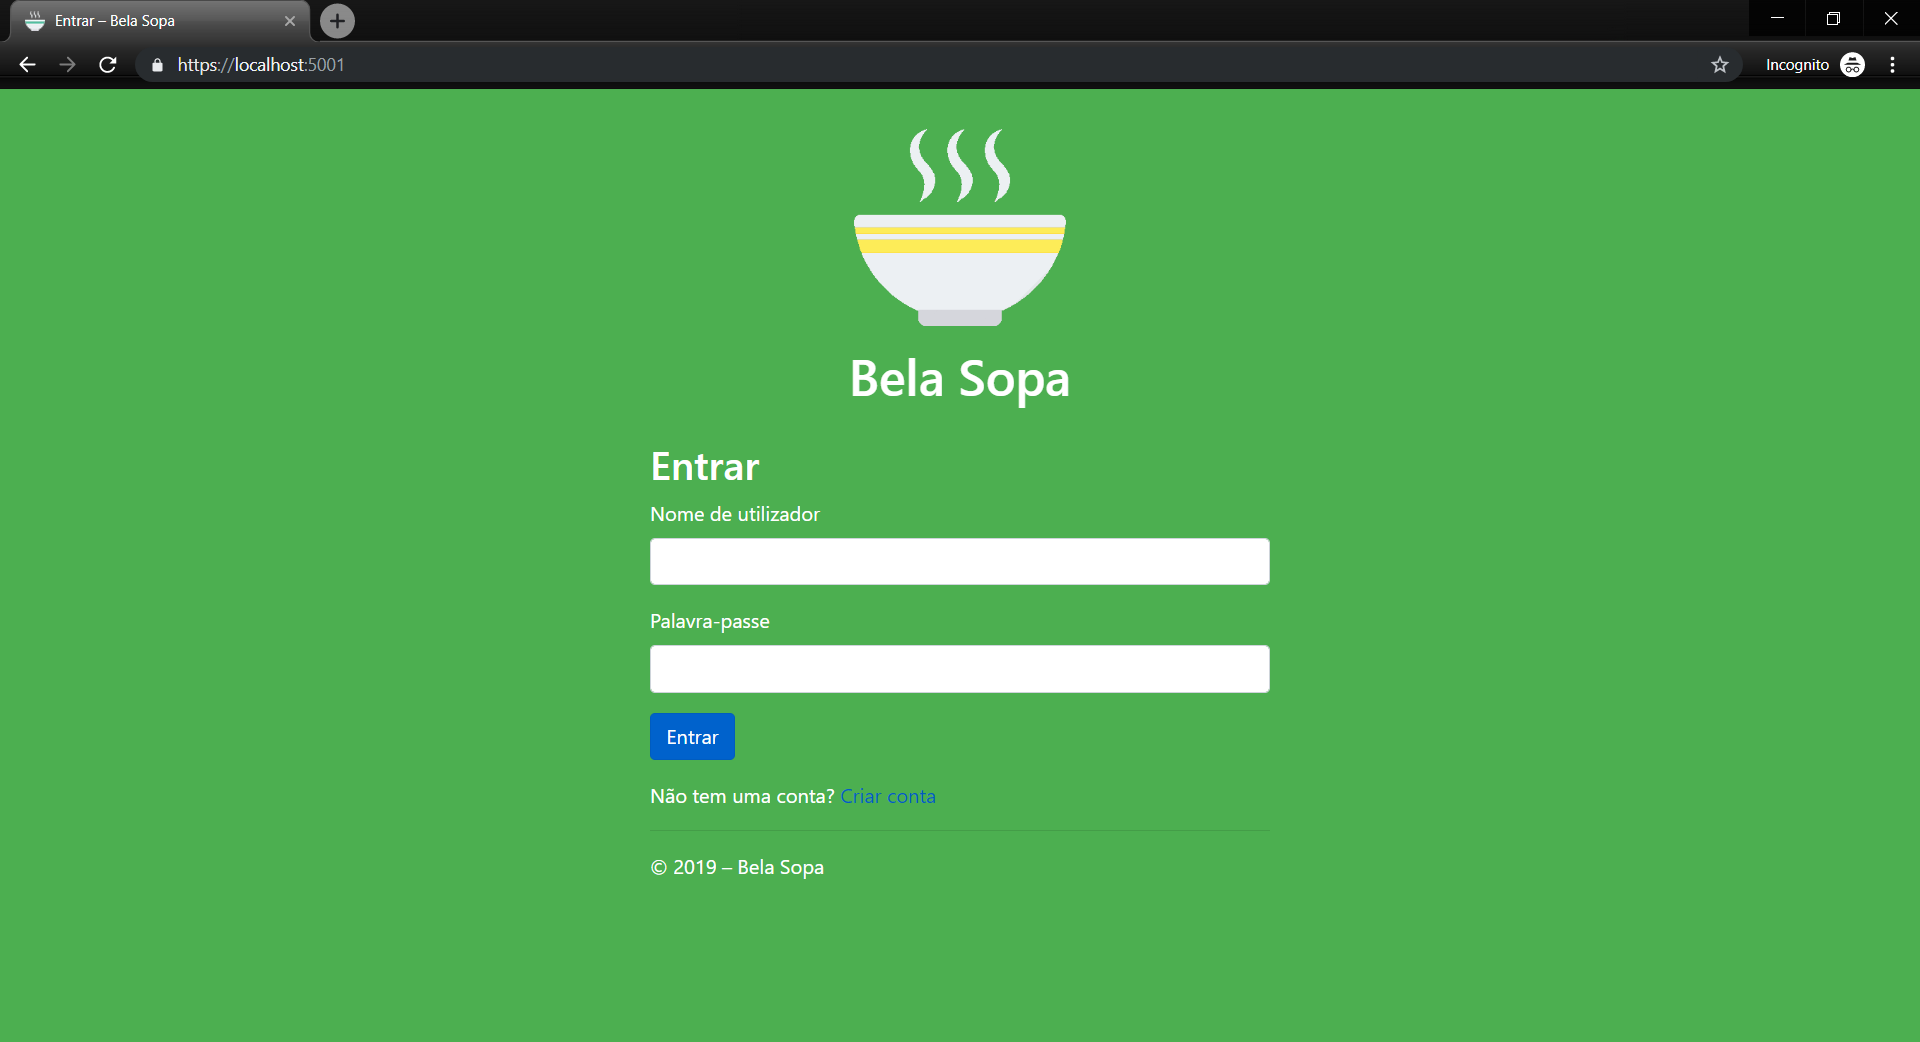
\includegraphics[height=.85\textheight]{figures/11/final-1.png}
  \caption{Aspeto final da interface de autenticação.}
  \label{fig:construcao:final-1}
\end{figure}

\begin{figure}[p]
  \centering
  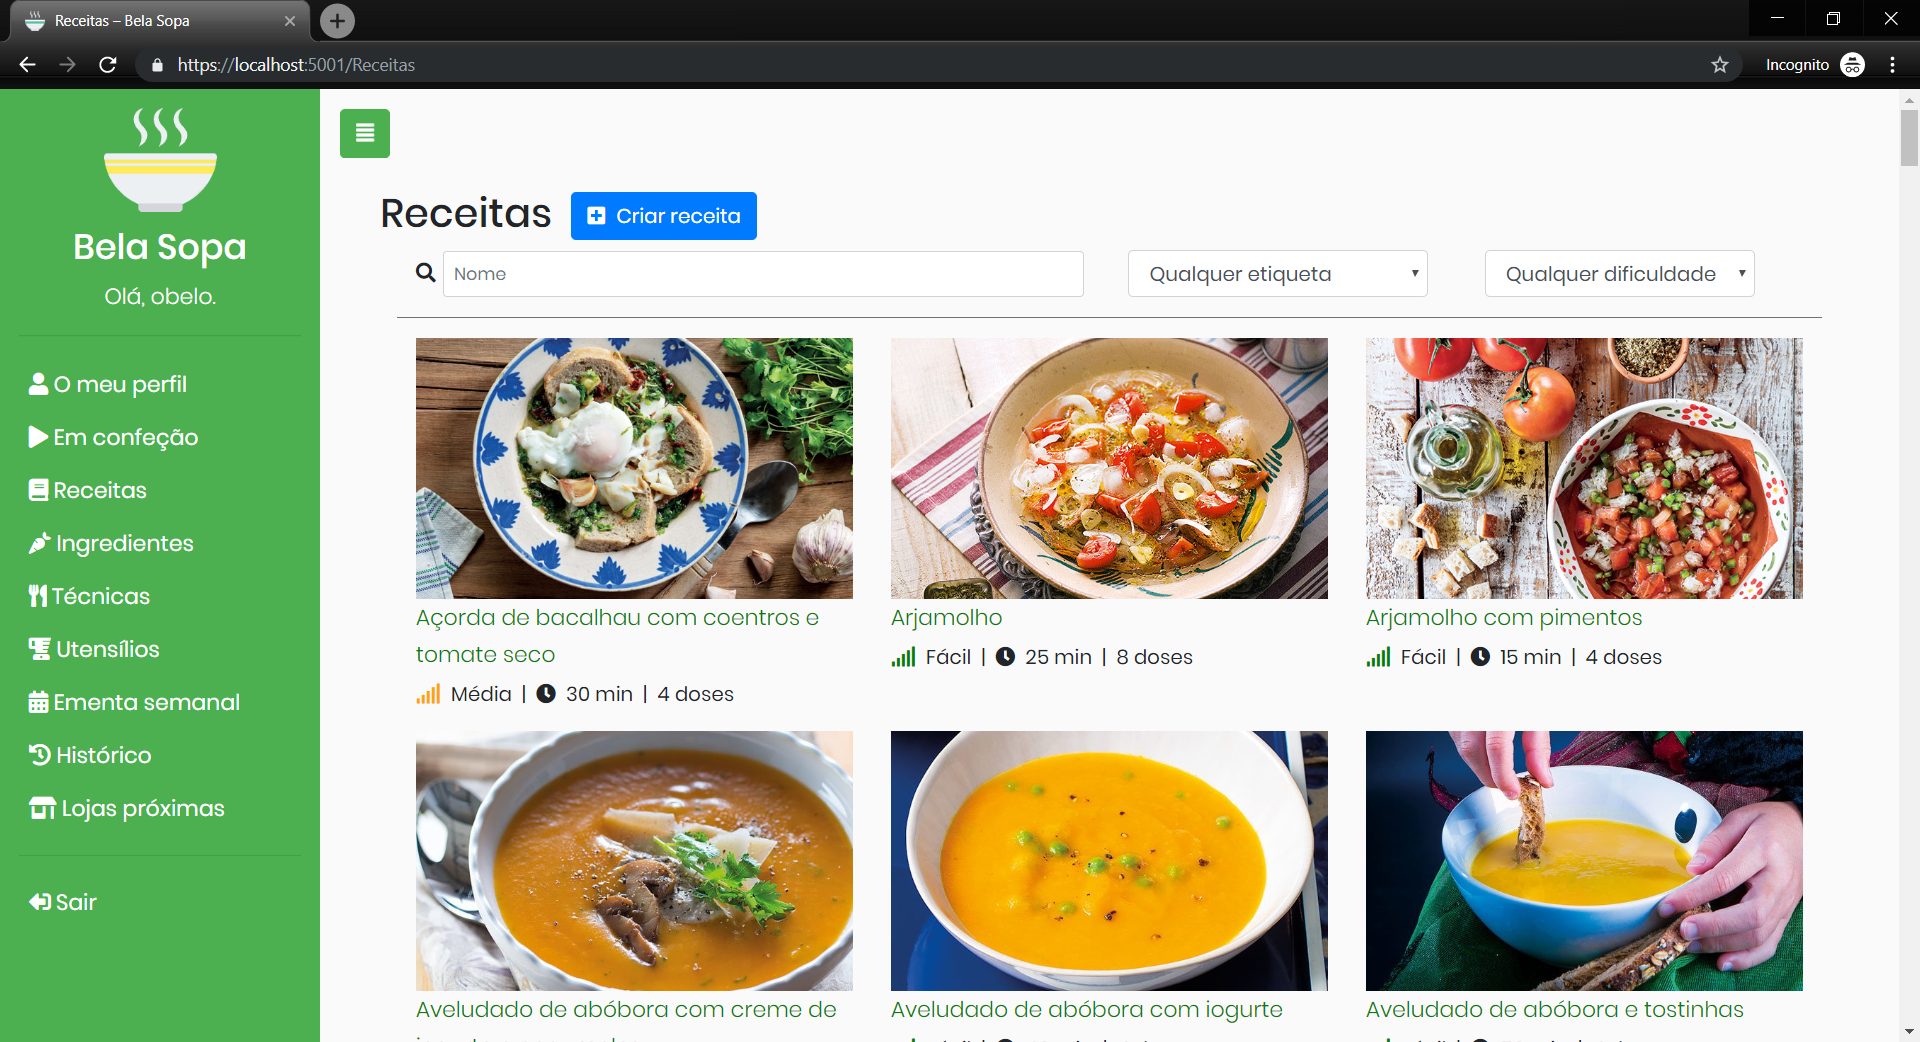
\includegraphics[height=.85\textheight]{figures/11/final-2.png}
  \caption{Aspeto final da interface de listagem de receitas.}
  \label{fig:construcao:final-2}
\end{figure}

\begin{figure}[p]
  \centering
  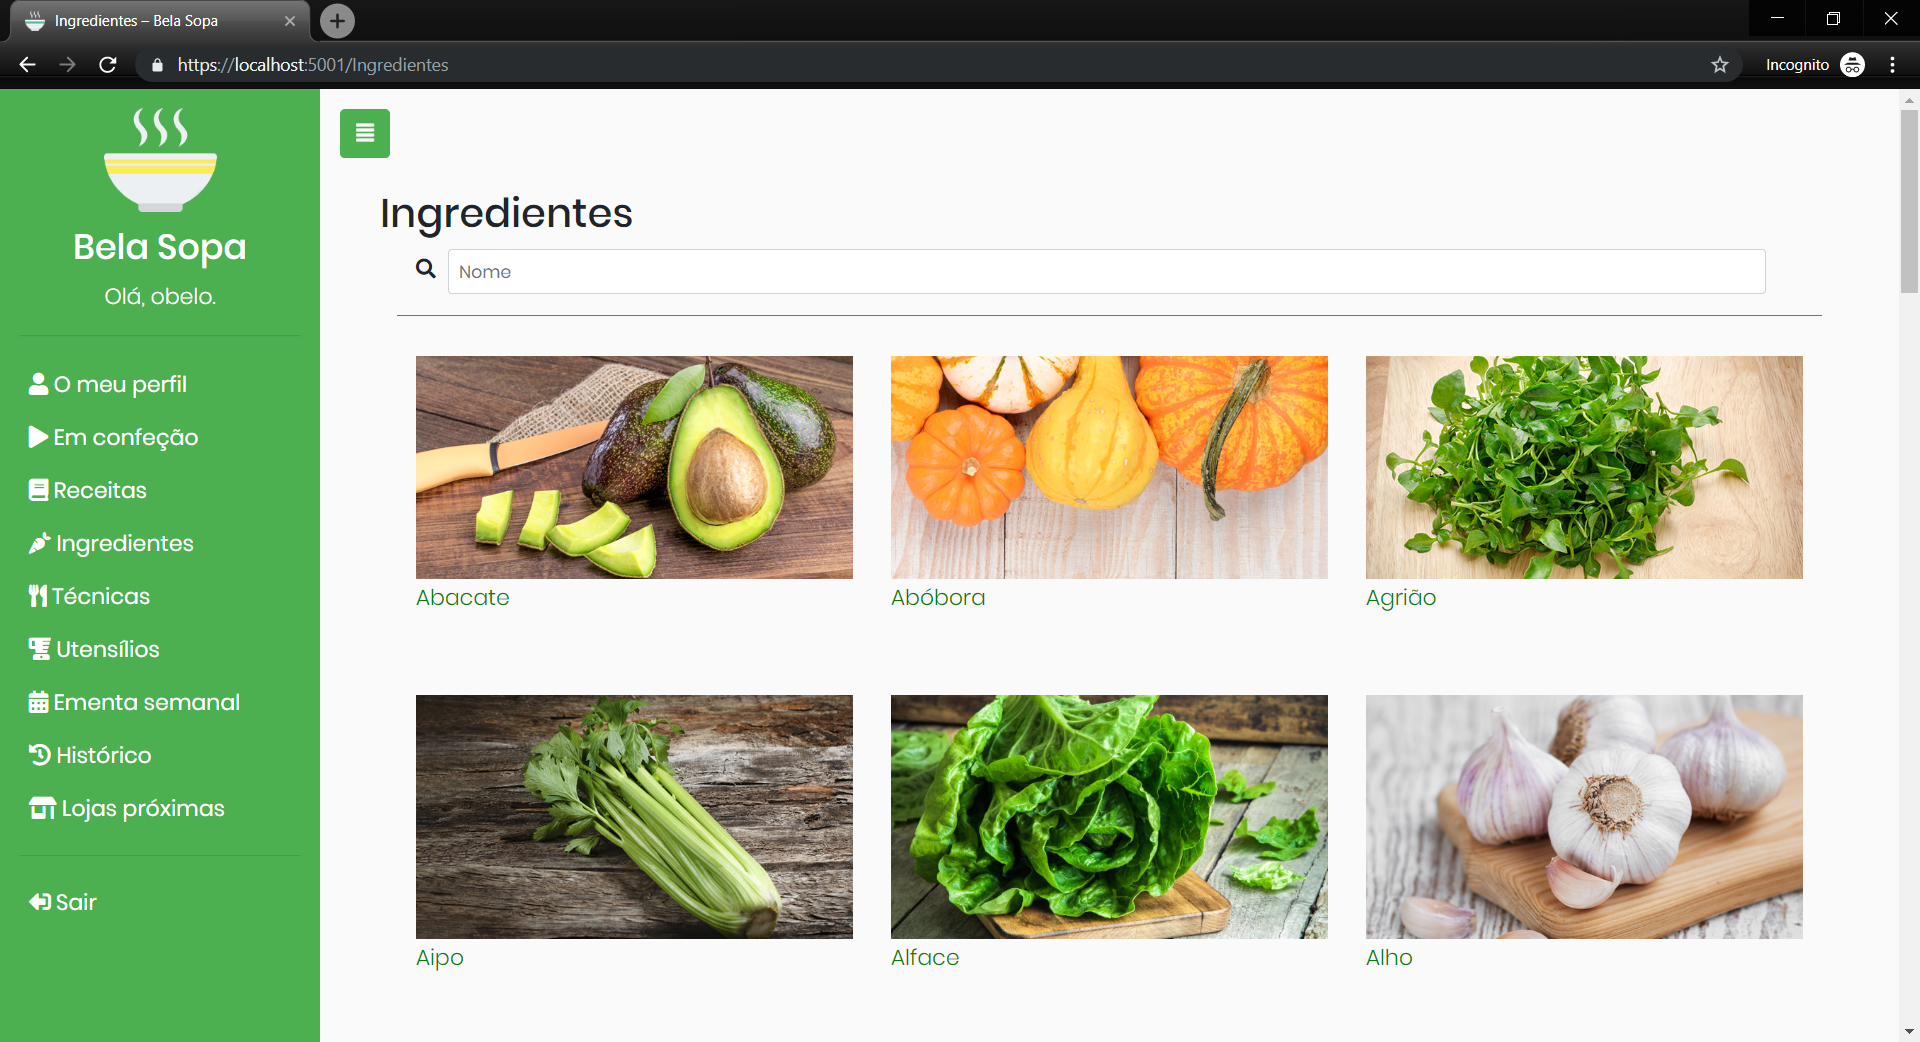
\includegraphics[height=.85\textheight]{figures/11/final-3.png}
  \caption{Aspeto final da interface de listagem de ingredientes.}
  \label{fig:construcao:final-3}
\end{figure}

\begin{figure}[p]
  \centering
  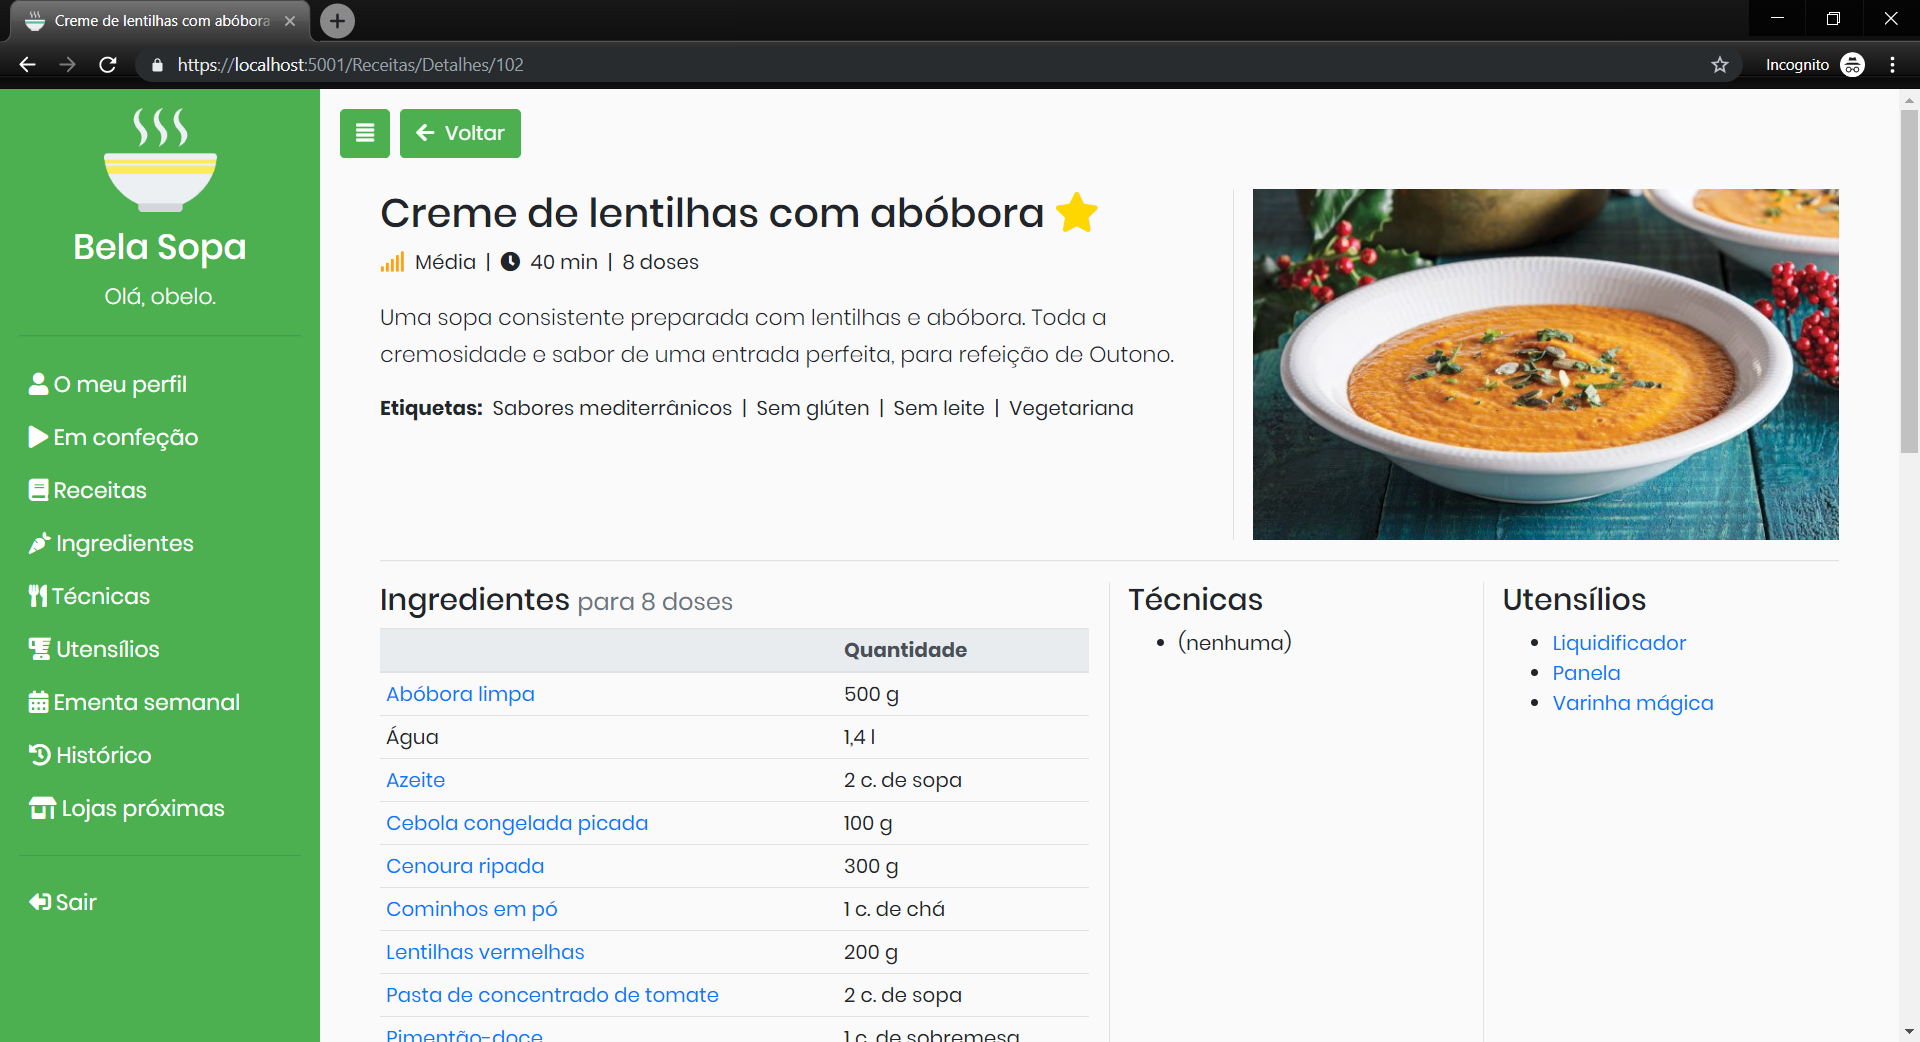
\includegraphics[height=.85\textheight]{figures/11/final-4.png}
  \caption{Aspeto final da interface de visualização de uma receita.}
  \label{fig:construcao:final-4}
\end{figure}

\end{landscape}

% ---------------------------------------------------------------------------- %

% ---------------------------------------------------------------------------- %

\section{Conclusões e Trabalho Futuro}
\label{cap:conclusao}

% Neste relatório apresentaram-se as fases de fundamentação e especificação do assistente pessoal de cozinha \emph{Bela Sopa}, cujo desenvolvimento foi encomendado pela cadeia de supermercados e hipermercados \emph{Gota Doce}. O sistema é baseado no serviço \emph{online} \ESCOLADECOZINHA, detido pela mesma empresa.

Neste relatório apresentou-se o trabalho prático realizado no âmbito da Unidade Curricular de Laboratórios de Informática IV, do curso de Mestrado Integrado em Engenharia Informática da Universidade do Minho, no ano letivo de 2018/2019. O caso de estudo considerado centra-se no desenvolvimento do assistente pessoal de cozinha \emph{Bela Sopa}, encomendado pela cadeia de supermercados e hipermercados \emph{Gota Doce}.

Foi primeiramente fundamentada a construção do sistema tendo em conta a sua utilidade e viabilidade, tendo-se também elaborado um plano para o seu desenvolvimento. Verificado-se que a construção do sistema seria vantajosa e que o seu processo de desenvolvimento cumpriria o orçamento e prazos estabelecidos, procedeu-se à fase de especificação do mesmo.

O trabalho realizado nessa mesma fase foi em seguida pormenorizado, apresentando-se com particular detalhe os resultados dos processos de modelação de domínio, levantamento e análise de requisitos, modelação de \emph{use cases}, prototipagem da interface de utilizador e modelação da arquitetura interna do sistema.

Por fim, descreveu-se o processo de construção do sistema e apresentou-se o produto resultante, enumerando-se também as tecnologias nas quais este se baseia e especificando-se o procedimento de instalação do sistema.

Devido a restrições de tempo, algumas funcionalidades delineadas na fase de especificação do sistema não foram concretizadas aquando da sua construção. Em particular, embora as receitas confecionadas e respetiva avaliação e dificuldade reportadas pelo utilizador sejam armazenadas e exibidas no seu histórico pessoal, esta informação não é utilizada para filtrar ou organizar a lista de receitas do sistema apresentada ao mesmo. Adicionalmente, a funcionalidade de visualização de lojas próximas poderá ser estendida com a capacidade de indicar trajetos até uma determinada loja. A implementação destas funcionalidades omissas constitui trabalho futuro.

Provando-se a adequação do sistema construído e o cumprimento dos seus objetivos, será considerado o alargamento do seu âmbito a formas de culinária além da confeção de sopas. Esta evolução é também identificada como trabalho futuro.

% Em particular, caso o utilizador declare que não tem todos os ingredientes necessários a uma determinada receita, o sistema não fornece diretamente informação sobre os locais onde os pode adquirir e os respetivos preços, embora o utilizador possa determinar a localização.

% ---------------------------------------------------------------------------- %


\printbibliography

% ---------------------------------------------------------------------------- %

\section*{Lista de Siglas e Acrónimos}

{\renewcommand{\arraystretch}{1}
\begin{tabular}{ @{} l @{\hskip 18pt} l }
  API & \emph{Application Programming Interface} \\
  MVC & \emph{Model-View-Controller} \\
  UML & \emph{Unified Modeling Language} \\
\end{tabular}}

% ---------------------------------------------------------------------------- %


\appendix
\renewcommand{\thesection}{Anexo \Roman{section}}

% ---------------------------------------------------------------------------- %

\section{Especificação dos \emph{Use Cases}}
\label{ane:use-cases-spec}

Incluem-se neste anexo as especificações de todos os \emph{use cases} identificados no \refcap{cap:use-cases}, excetuando-se aquelas já apresentadas nesse mesmo capítulo.

% ---------------------------------------------------------------------------- %

\begin{table}[ht]
  \centering
  \tabelausecase
  \begin{tabularx}{\textwidth}{|>{\raggedright\let\newline\\\arraybackslash\hspace{0pt}}p{2.5cm}|>{\raggedright\let\newline\\\arraybackslash\hspace{0pt}}X|>{\raggedright\let\newline\\\arraybackslash\hspace{0pt}}X|}
    \hline
    \emph{Use case}: & \multicolumn{2}{l|}{Aceder a serviços externos} \\ \hline
    Pré-condição: & \multicolumn{2}{l|}{Estar autenticado} \\ \hline
    Pós-condição: & \multicolumn{2}{l|}{Acedeu ao serviço externo e estado do sistema não é alterado} \\ \hline
     & \textbf{Ator} & \textbf{Sistema} \\ \hline
    \multirow[t]{3}{=}{Comportamento Normal} & 1. Escolhe aceder a serviços externos &  \\ \cline{2-3}
     &  & 2. Guarda o estado da aplicação \\ \cline{2-3}
     &  & 3. Redireciona para a aplicação dos serviços externos \\ \hline
\end{tabularx}
  \caption{Especificação do \emph{use case} ``aceder a serviços externos''.}
  \label{tab:uc-aceder-a-servicos-externos}
\end{table}

% ---------------------------------------------------------------------------- %

% ---------------------------------------------------------------------------- %

\begin{table}[ht]
  \centering
  \tabelausecase
  \begin{tabularx}{\textwidth}{|>{\raggedright\let\newline\\\arraybackslash\hspace{0pt}}p{2.5cm}|>{\raggedright\let\newline\\\arraybackslash\hspace{0pt}}X|>{\raggedright\let\newline\\\arraybackslash\hspace{0pt}}X|}
    \hline
    \emph{Use case}: & \multicolumn{2}{l|}{Adicionar receita aos favoritos} \\ \hline
    Pré-condição: & \multicolumn{2}{l|}{Estar autenticado} \\ \hline
    Pós-condição: & \multicolumn{2}{l|}{Receita foi adicionada aos favoritos} \\ \hline
     & \textbf{Ator} & \textbf{Sistema} \\ \hline
    \multirow[t]{4}{=}{Comportamento Normal} & 1. Escolhe adicionar a receita ao favoritos &  \\ \cline{2-3}
     &  & 2. Valida inserção \\ \cline{2-3}
     &  & 3. Insere receita aos favoritos \\ \cline{2-3}
     &  & 4. Informa que inseriu a receita com sucesso \\ \hline
    Exceção 1 [Receita já está nos favoritos] (passo 3) &  & 3.1. Informa que a receita está nos favoritos \\ \hline
\end{tabularx}
  \caption{Especificação do \emph{use case} ``adicionar receita aos favoritos''.}
  \label{tab:uc-adicionar-receita-aos-favoritos}
\end{table}

% ---------------------------------------------------------------------------- %

% ---------------------------------------------------------------------------- %

\begin{table}[ht]
  \centering
  \tabelausecase
  \begin{tabularx}{\textwidth}{|>{\raggedright\let\newline\\\arraybackslash\hspace{0pt}}p{2.5cm}|>{\raggedright\let\newline\\\arraybackslash\hspace{0pt}}X|>{\raggedright\let\newline\\\arraybackslash\hspace{0pt}}X|}
    \hline
    \emph{Use case}: & \multicolumn{2}{l|}{Apagar conta} \\ \hline
    Pré-condição: & \multicolumn{2}{l|}{Estar autenticado} \\ \hline
    Pós-condição: & \multicolumn{2}{l|}{Conta eliminada} \\ \hline
     & \textbf{Ator} & \textbf{Sistema} \\ \hline
    \multirow[t]{3}{=}{Comportamento Normal} & 1. Fornece o email da conta que pretende ser apaga. &  \\ \cline{2-3}
     &  & 2. Valida email \\ \cline{2-3}
     &  & 3. Elimina conta \\ \hline
    \multirow[t]{2}{=}{Comportamento Alternativo 1 [Ator é cliente] (passo 2)} &  & 2.1. Valida se a conta é do próprio \\ \cline{2-3}
     &  & 2.2. Elimina conta \\ \hline
    Exceção 1 [Email de cliente inválido] (passo 2) &  & 2.1. Informa que o email é inválido \\ \hline
    Exceção 2 [Dados inválidos] (passo 2) &  & 2.1. Informa que o email é invalido \\ \hline
\end{tabularx}
  \caption{Especificação do \emph{use case} ``apagar conta''.}
  \label{tab:uc-apagar-conta}
\end{table}

% ---------------------------------------------------------------------------- %

% ---------------------------------------------------------------------------- %

\begin{table}[ht]
  \centering
  \tabelausecase
  \begin{tabularx}{\textwidth}{|>{\raggedright\let\newline\\\arraybackslash\hspace{0pt}}p{2.5cm}|>{\raggedright\let\newline\\\arraybackslash\hspace{0pt}}X|>{\raggedright\let\newline\\\arraybackslash\hspace{0pt}}X|}
    \hline
    \emph{Use case}: & \multicolumn{2}{l|}{Consultar ou editar informação da conta} \\ \hline
    Pré-condição: & \multicolumn{2}{l|}{Estar autenticado} \\ \hline
    Pós-condição: & \multicolumn{2}{l|}{Dados consultados} \\ \hline
     & \textbf{Ator} & \textbf{Sistema} \\ \hline
    \multirow[t]{3}{=}{Comportamento Normal} & 1. Consulta perfil &  \\ \cline{2-3}
     &  & 2. Mostra o perfil do ator \\ \cline{2-3}
     & 3. Conclui Consulta &  \\ \hline
    \multirow[t]{3}{=}{Comportamento Alternativo 1 [Ator edita perfil] (passo 3)} & 3.1. Edita perfil &  \\ \cline{2-3}
     &  & 3.2. <<include>> Apagar Conta \\ \cline{2-3}
     &  & 3.3. <<include>> Registar Conta \\ \hline
\end{tabularx}
  \caption{Especificação do \emph{use case} ``consultar ou editar informação da conta''.}
  \label{tab:uc-consultar-ou-editar-informacao-da-conta}
\end{table}

% ---------------------------------------------------------------------------- %

% ---------------------------------------------------------------------------- %

\begin{table}[ht]
  \centering
  \tabelausecase
  \begin{tabularx}{\textwidth}{|>{\raggedright\let\newline\\\arraybackslash\hspace{0pt}}p{2.5cm}|>{\raggedright\let\newline\\\arraybackslash\hspace{0pt}}X|>{\raggedright\let\newline\\\arraybackslash\hspace{0pt}}X|}
    \hline
    \emph{Use case}: & \multicolumn{2}{l|}{Consultar Receita} \\ \hline
    Pré-condição: & \multicolumn{2}{l|}{Estar autenticado, receita existe} \\ \hline
    Pós-condição: & \multicolumn{2}{l|}{Receita foi consultada} \\ \hline
     & \textbf{Ator} & \textbf{Sistema} \\ \hline
    \multirow[t]{3}{=}{Comportamento Normal} & 1. Escolhe receita que deseja consultar &  \\ \cline{2-3}
     &  & 2. Mostra a descrição, as imagens, a porção, os utensílios, ,os ingredientes, etc… \\ \cline{2-3}
     & 3. <<extends>> Confecionar receita &  \\ \hline
\end{tabularx}
  \caption{Especificação do \emph{use case} ``consultar receita''.}
  \label{tab:uc-consultar-receita}
\end{table}

% ---------------------------------------------------------------------------- %

% ---------------------------------------------------------------------------- %

\begin{table}[ht]
  \centering
  \tabelausecase
  \begin{tabularx}{\textwidth}{|>{\raggedright\let\newline\\\arraybackslash\hspace{0pt}}p{2.5cm}|>{\raggedright\let\newline\\\arraybackslash\hspace{0pt}}X|>{\raggedright\let\newline\\\arraybackslash\hspace{0pt}}X|}
    \hline
    \emph{Use case}: & \multicolumn{2}{l|}{Editar ementa semanal} \\ \hline
    Pré-condição: & \multicolumn{2}{l|}{Estar autenticado} \\ \hline
    Pós-condição: & \multicolumn{2}{l|}{Ementa semanal foi alterada} \\ \hline
     & \textbf{Ator} & \textbf{Sistema} \\ \hline
    \multirow[t]{2}{=}{Comportamento Normal} &  & 1. Mostra todas as receitas na ementa nos dias e refeições já escolhidas \\ \cline{2-3}
     &  & 2. <<extends>> adicionar receita à ementa \\ \hline
    Comportamento Alternativo 1 [Escolhe remover uma receita] (passo 2) &  & 2.1. <<extends>> remover receita da ementa \\ \hline
\end{tabularx}
  \caption{Especificação do \emph{use case} ``editar ementa semanal''.}
  \label{tab:uc-editar-ementa-semanal}
\end{table}

% ---------------------------------------------------------------------------- %

% ---------------------------------------------------------------------------- %

\begin{table}[ht]
  \centering
  \tabelausecase
  \begin{tabularx}{\textwidth}{|>{\raggedright\let\newline\\\arraybackslash\hspace{0pt}}p{2.5cm}|>{\raggedright\let\newline\\\arraybackslash\hspace{0pt}}X|>{\raggedright\let\newline\\\arraybackslash\hspace{0pt}}X|}
    \hline
    \emph{Use case}: & \multicolumn{2}{l|}{Gerar lista de ingredientes} \\ \hline
    Pré-condição: & \multicolumn{2}{l|}{Estar autenticado} \\ \hline
    Pós-condição: & \multicolumn{2}{l|}{Lista de ingredientes guardada no sistema} \\ \hline
     & \textbf{Ator} & \textbf{Sistema} \\ \hline
    \multirow[t]{7}{=}{Comportamento Normal} & 1. Decide gerar a lista de ingredientes &  \\ \cline{2-3}
     &  & 2. Consulta ementa semanal do ator \\ \cline{2-3}
     &  & 3. Calcula os ingredientes necessários para a semana \\ \cline{2-3}
     &  & 4. Mostra os ingredientes e as respetivas quantidades \\ \cline{2-3}
     & 5. Confirma a lista de ingredientes. &  \\ \cline{2-3}
     &  & 6. Guarda a lista de ingredientes \\ \cline{2-3}
     & 7. <<extends>> aceder a serviços externos &  \\ \hline
    \multirow[t]{3}{=}{Comportamento Alternativo 1 [Ator quer adicionar ingrediente à lista] (passo 5)} & 5.1. Escolhe o ingrediente e quantidade a adicionar &  \\ \cline{2-3}
     &  & 5.2. Adiciona ingrediente à lista \\ \cline{2-3}
     &  & 5.3. Volta ao passo 5 \\ \hline
    \multirow[t]{3}{=}{Comportamento Alternativo 2 [Ator quer remover ingredientes à lista] (passo 5)} & 5.1. Escolhe o ingrediente e quantidade a remover &  \\ \cline{2-3}
     &  & 5.2. Remove ingrediente da lista \\ \cline{2-3}
     &  & 5.3. Volta ao passo 5 \\ \hline
    \multirow[t]{2}{=}{Comportamento Alternativo 3 [Quantidade do ingrediente é zero] (passo 5.2)} &  & 5.2.1 Indica que o ingrediente não existe na lista \\ \cline{2-3}
     &  & 5.2.2 Volta ao passo 5 \\ \hline
\end{tabularx}
  \caption{Especificação do \emph{use case} ``gerar lista de ingredientes''.}
  \label{tab:uc-gerar-lista-de-ingredientes}
\end{table}

% ---------------------------------------------------------------------------- %

% ---------------------------------------------------------------------------- %

\begin{table}[ht]
  \centering
  \tabelausecase
  \begin{tabularx}{\textwidth}{|>{\raggedright\let\newline\\\arraybackslash\hspace{0pt}}p{2.5cm}|>{\raggedright\let\newline\\\arraybackslash\hspace{0pt}}X|>{\raggedright\let\newline\\\arraybackslash\hspace{0pt}}X|}
    \hline
    \emph{Use case}: & \multicolumn{2}{l|}{Pedir ajuda} \\ \hline
    Pré-condição: & \multicolumn{2}{l|}{Estar autenticado} \\ \hline
    Pós-condição: & \multicolumn{2}{l|}{} \\ \hline
     & \textbf{Ator} & \textbf{Sistema} \\ \hline
    \multirow[t]{3}{=}{Comportamento Normal} & 1. Solicita ajuda num certo conceito &  \\ \cline{2-3}
     &  & 2. Procura conceito \\ \cline{2-3}
     &  & 3. Mostra uma descrição, e possivelmente uma imagem e/ou video sobre o conceito \\ \hline
    Exceção 1 [Não existe conceito] (passo 2) &  & 2.1. Informa que não é possível encontrar esse conceito \\ \hline
\end{tabularx}
  \caption{Especificação do \emph{use case} ``pedir ajuda''.}
  \label{tab:uc-pedir-ajuda}
\end{table}

% ---------------------------------------------------------------------------- %

% ---------------------------------------------------------------------------- %

\begin{table}[ht]
  \centering
  \tabelausecase
  \begin{tabularx}{\textwidth}{|>{\raggedright\let\newline\\\arraybackslash\hspace{0pt}}p{2.5cm}|>{\raggedright\let\newline\\\arraybackslash\hspace{0pt}}X|>{\raggedright\let\newline\\\arraybackslash\hspace{0pt}}X|}
    \hline
    \emph{Use case}: & \multicolumn{2}{l|}{Remover receita dos favoritos} \\ \hline
    Pré-condição: & \multicolumn{2}{l|}{Estar autenticado} \\ \hline
    Pós-condição: & \multicolumn{2}{l|}{Receita foi removida aos favoritos} \\ \hline
     & \textbf{Ator} & \textbf{Sistema} \\ \hline
    \multirow[t]{4}{=}{Comportamento Normal} & 1. Escolhe remover a receita dos favoritos &  \\ \cline{2-3}
     &  & 2. Valida remoção \\ \cline{2-3}
     &  & 3. Remove receita dos favoritos \\ \cline{2-3}
     &  & 4. Informa que removeu a receita com sucesso \\ \hline
    Exceção 1 [Receita não se encontra nos favoritos] (passo 3) &  & 3.1. Informa que a receita não está nos favoritos \\ \hline
\end{tabularx}
  \caption{Especificação do \emph{use case} ``remover receita dos favoritos''.}
  \label{tab:uc-remover-receita-dos-favoritos}
\end{table}

% ---------------------------------------------------------------------------- %

% ---------------------------------------------------------------------------- %

\begin{table}[ht]
  \centering
  \tabelausecase
  \begin{tabularx}{\textwidth}{|>{\raggedright\let\newline\\\arraybackslash\hspace{0pt}}p{2.5cm}|>{\raggedright\let\newline\\\arraybackslash\hspace{0pt}}X|>{\raggedright\let\newline\\\arraybackslash\hspace{0pt}}X|}
    \hline
    \emph{Use case}: & \multicolumn{2}{l|}{Ver loja mais próxima} \\ \hline
    Pré-condição: & \multicolumn{2}{l|}{Estar autenticado e existem lojas} \\ \hline
    Pós-condição: & \multicolumn{2}{l|}{foi encontrada uma loja} \\ \hline
     & \textbf{Ator} & \textbf{Sistema} \\ \hline
    \multirow[t]{3}{=}{Comportamento Normal} & 1. Solicita ver a loja mais perto de uma determinada localização &  \\ \cline{2-3}
     &  & 2. Calcula a loja mais perto das conhecidas \\ \cline{2-3}
     &  & 3. Mostra loja \\ \hline
\end{tabularx}
  \caption{Especificação do \emph{use case} ``ver loja mais próxima''.}
  \label{tab:uc-ver-loja-mais-proxima}
\end{table}

% ---------------------------------------------------------------------------- %


% ---------------------------------------------------------------------------- %

% ---------------------------------------------------------------------------- %

\section{Diagramas de Sequência para a Ca\-ma\-da de Negócio}
\label{ane:negocio-diag-seq}

Apresenta-se neste anexo os restantes diagramas de sequência que descrever o funcionamento, dos métodos que envolvem interação entre as componentes/classes da camada de negócio.

\begin{figure}[ht]
   \centering
   \includegraphics[width=\textwidth]{figures/10/Aceder_a_serviços_externos.pdf}
   \caption{Diagrama de sequência para o acesso a serviços externos.}
   \label{fig:negocio:DiagramaSequencia3}
 \end{figure}
 
 \begin{figure}[ht]
   \centering
   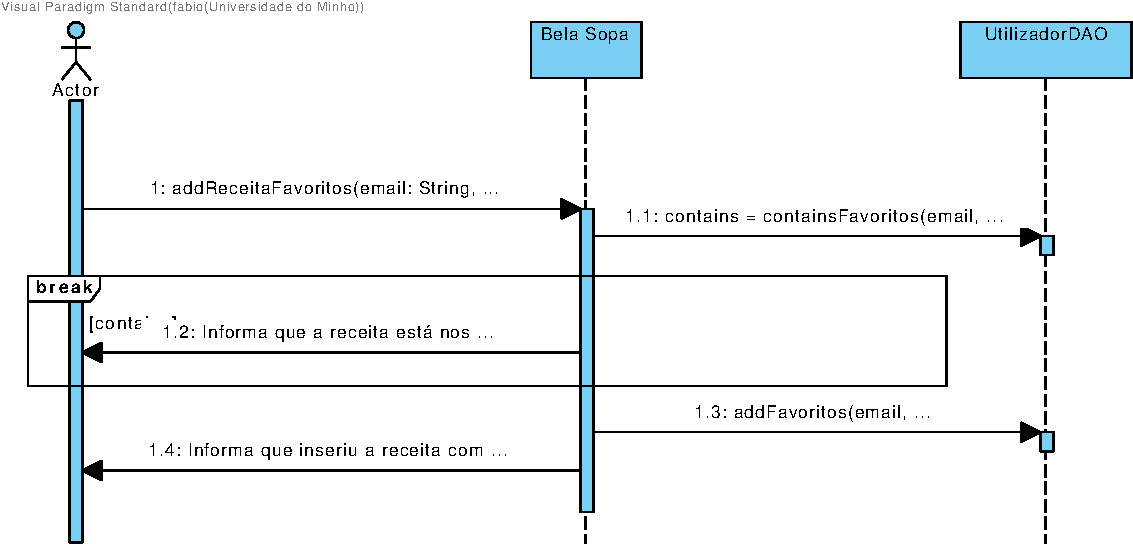
\includegraphics[width=\textwidth]{figures/10/Adicionar_receita_favoritos.pdf}
   \caption{Diagrama de sequência para o adicionar de uma receita aos favoritos.}
   \label{fig:negocio:DiagramaSequencia4}
 \end{figure}
 
 \begin{figure}[ht]
   \centering
   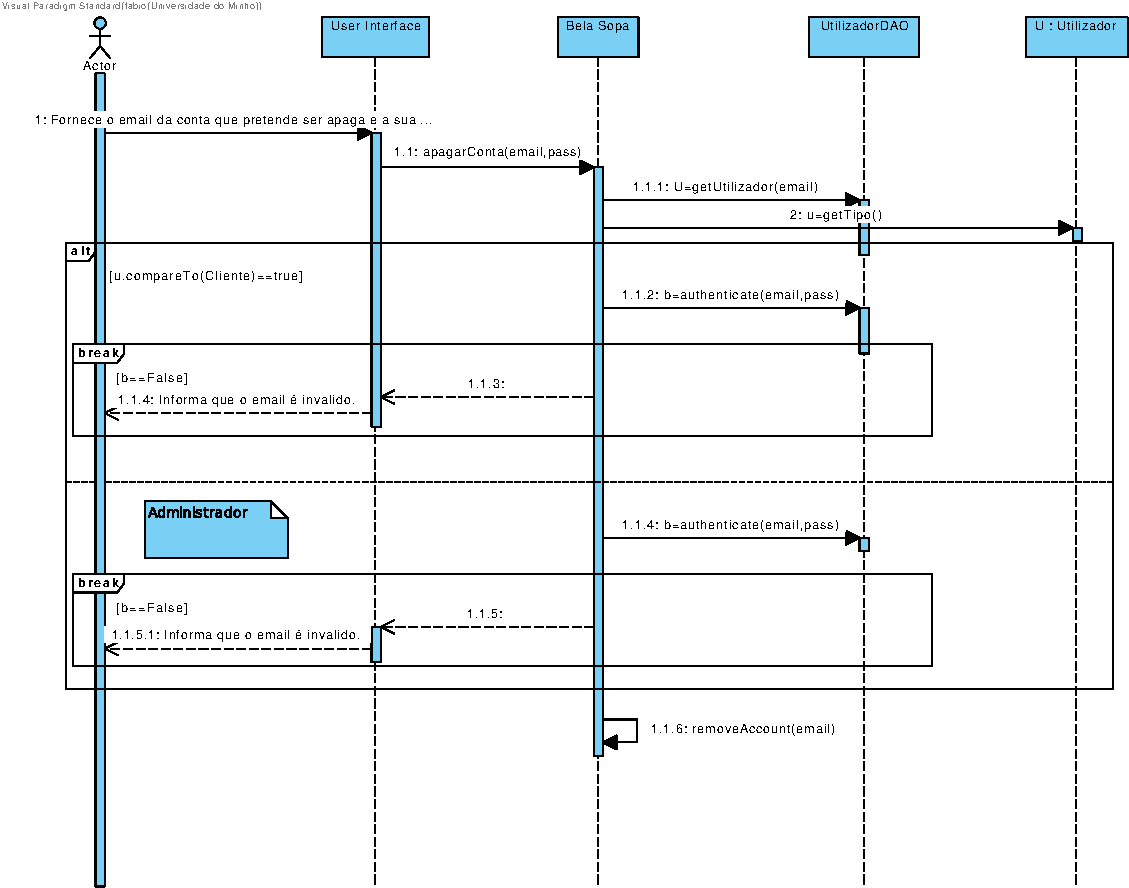
\includegraphics[width=\textwidth]{figures/10/Apagar_Conta.pdf}
   \caption{Diagrama de sequência para a remoção de uma conta.}
   \label{fig:negocio:DiagramaSequencia5}
 \end{figure}
 
 \begin{figure}[ht]
   \centering
   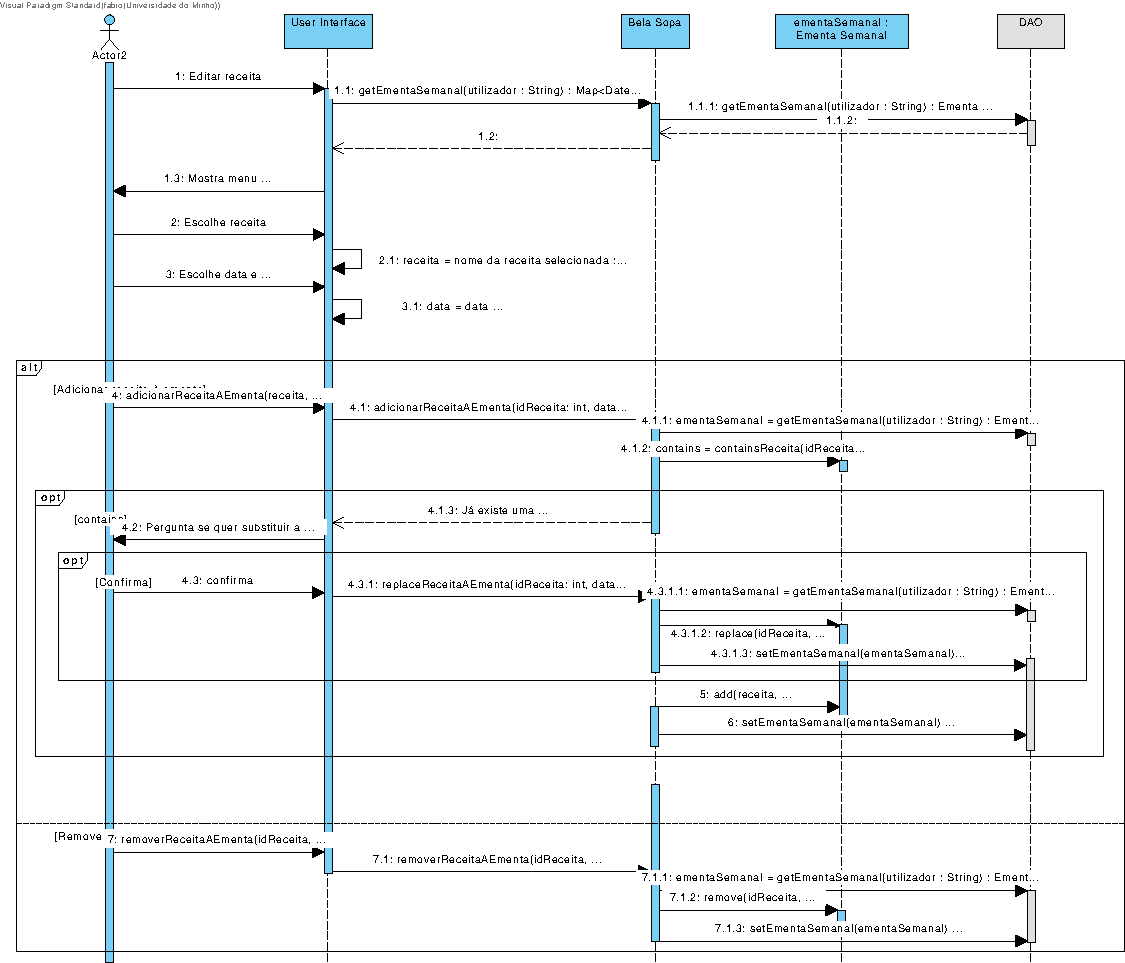
\includegraphics[width=\textwidth]{figures/10/Editar_ementa_semanal.pdf}
   \caption{Diagrama de sequência para a edição da ementa semanal.}
   \label{fig:negocio:DiagramaSequencia6}
 \end{figure}
 
 \begin{figure}[ht]
   \centering
   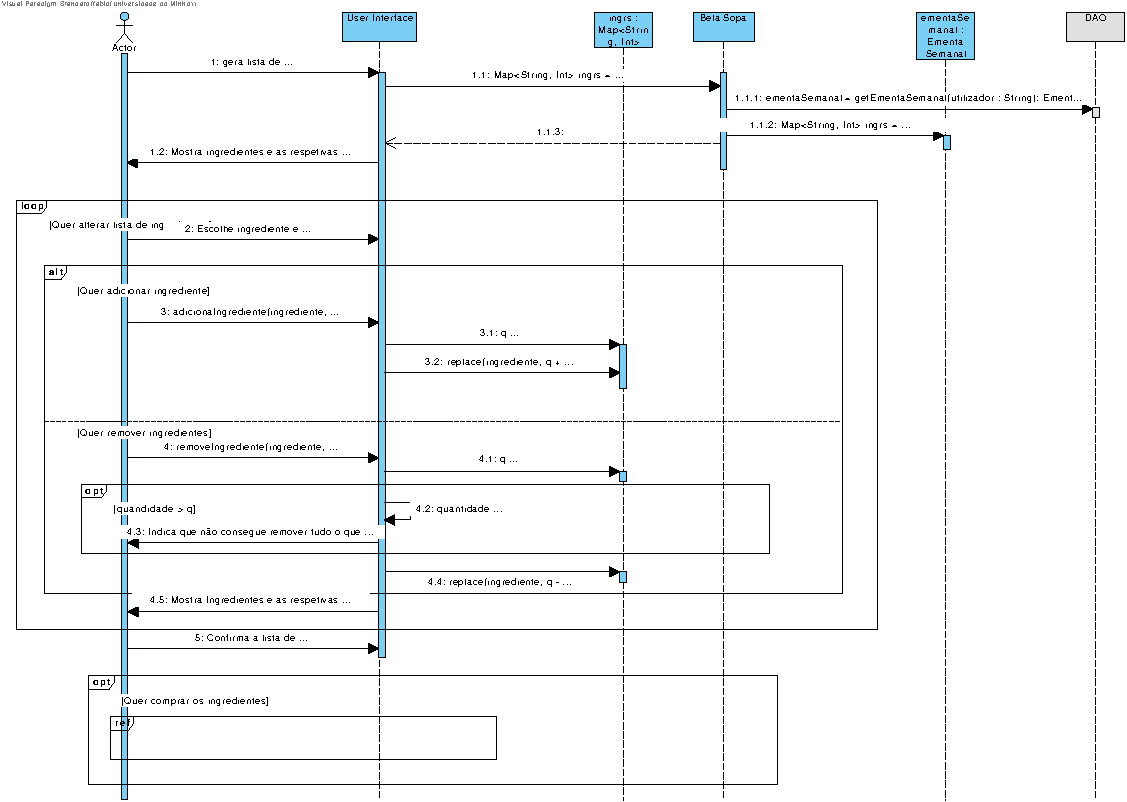
\includegraphics[width=\textwidth]{figures/10/Gerar_lista_de_ingredientes.pdf}
   \caption{Diagrama de sequência para a geração de uma lista de ingredientes.}
   \label{fig:negocio:DiagramaSequencia7}
 \end{figure}
 
 \begin{figure}[ht]
   \centering
   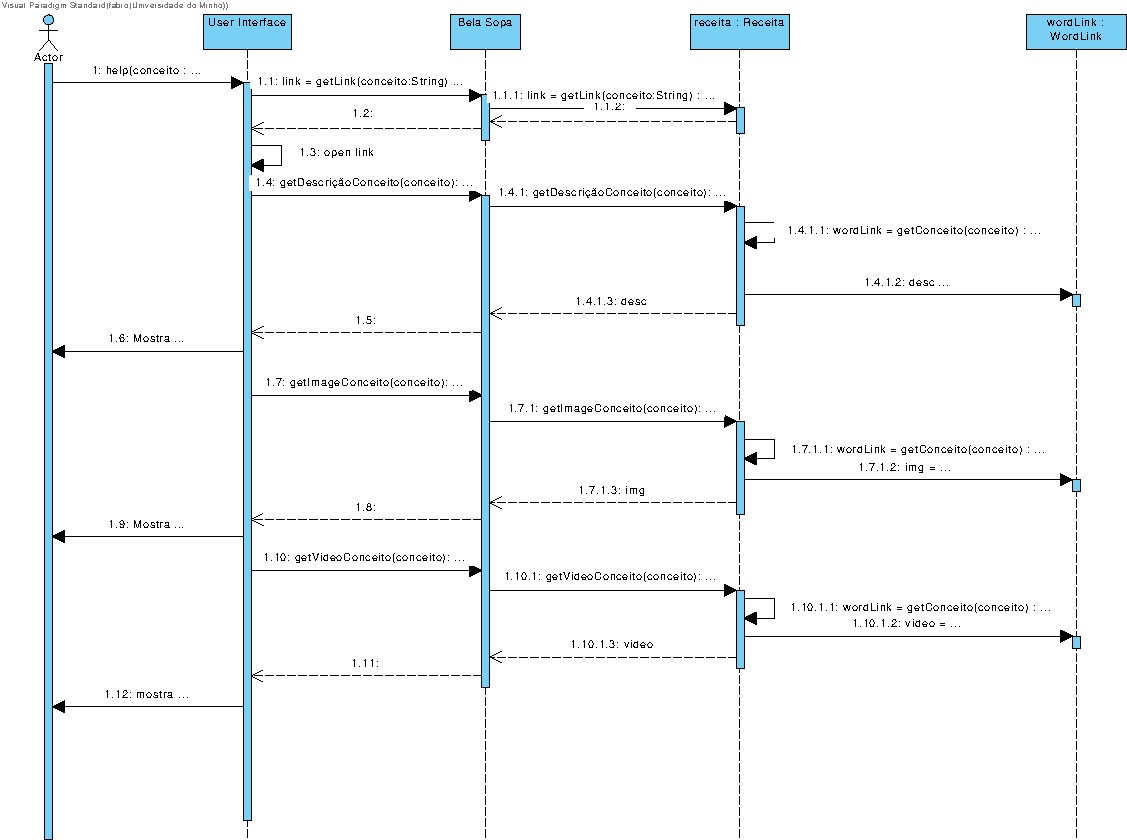
\includegraphics[width=\textwidth]{figures/10/Pedir_ajuda.pdf}
   \caption{Diagrama de sequência para o efetuar de um pedido de ajuda.}
   \label{fig:negocio:DiagramaSequencia8}
 \end{figure}
 
 \begin{figure}[ht]
   \centering
   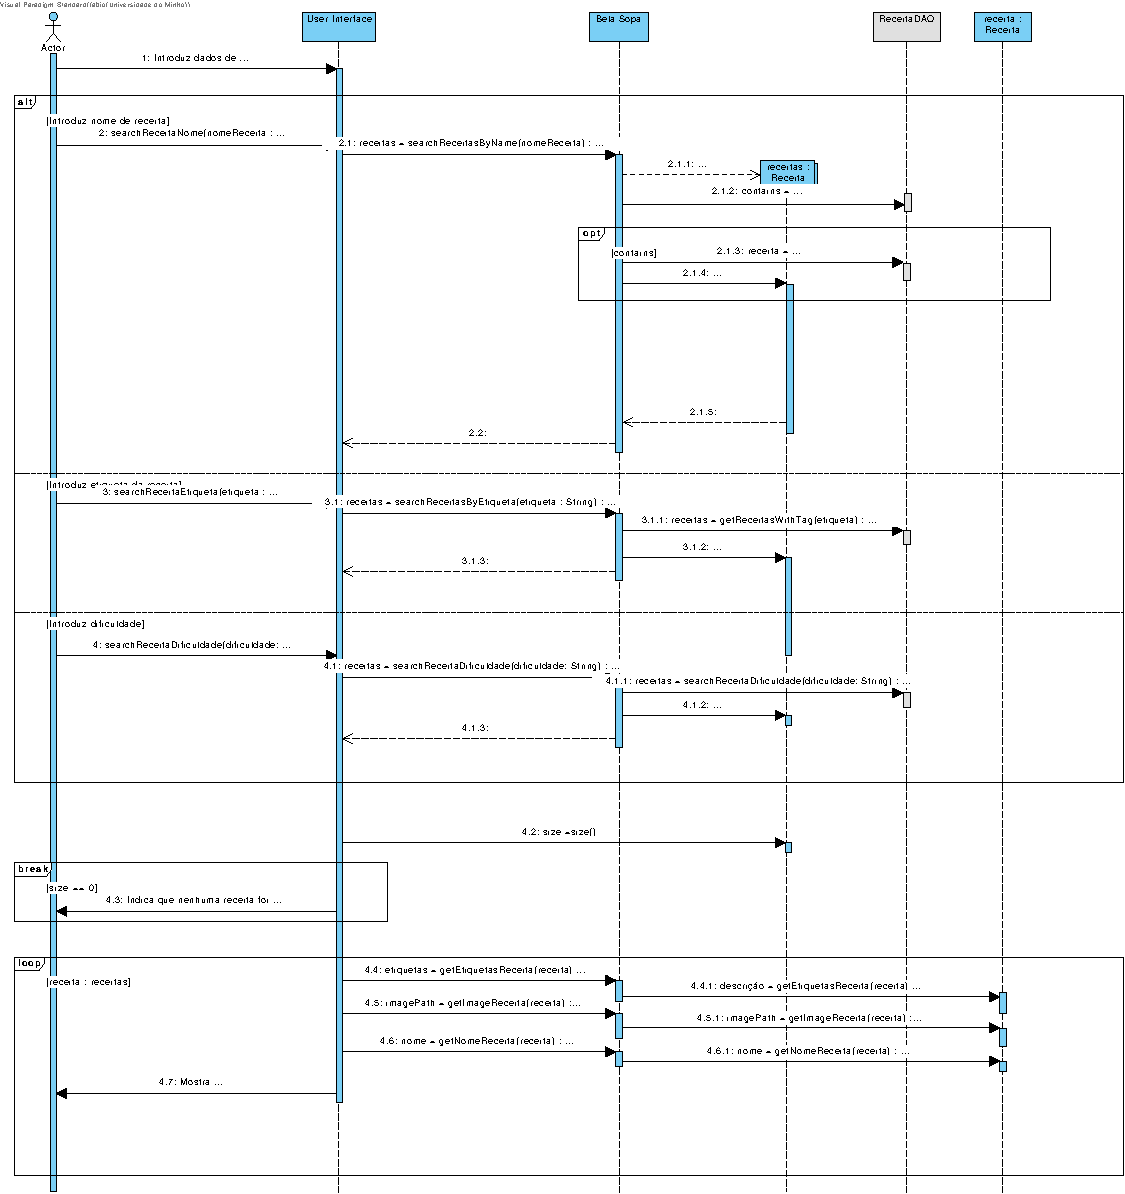
\includegraphics[width=\textwidth]{figures/10/Procurar_receita.pdf}
   \caption{Diagrama de sequência para a procura de uma receita.}
   \label{fig:negocio:DiagramaSequencia9}
 \end{figure}
 
 \begin{figure}[ht]
   \centering
   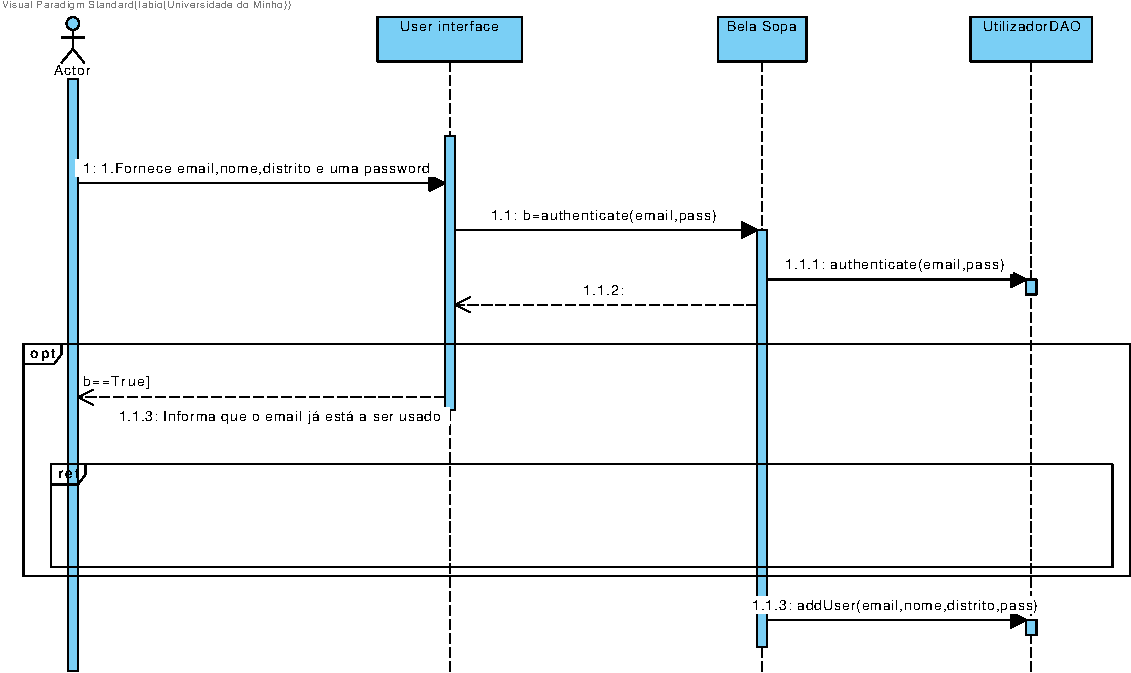
\includegraphics[width=\textwidth]{figures/10/Registar_Conta.pdf}
   \caption{Diagrama de sequência para a criação de uma conta.}
   \label{fig:negocio:DiagramaSequencia10}
 \end{figure}
 
 \begin{figure}[ht]
   \centering
   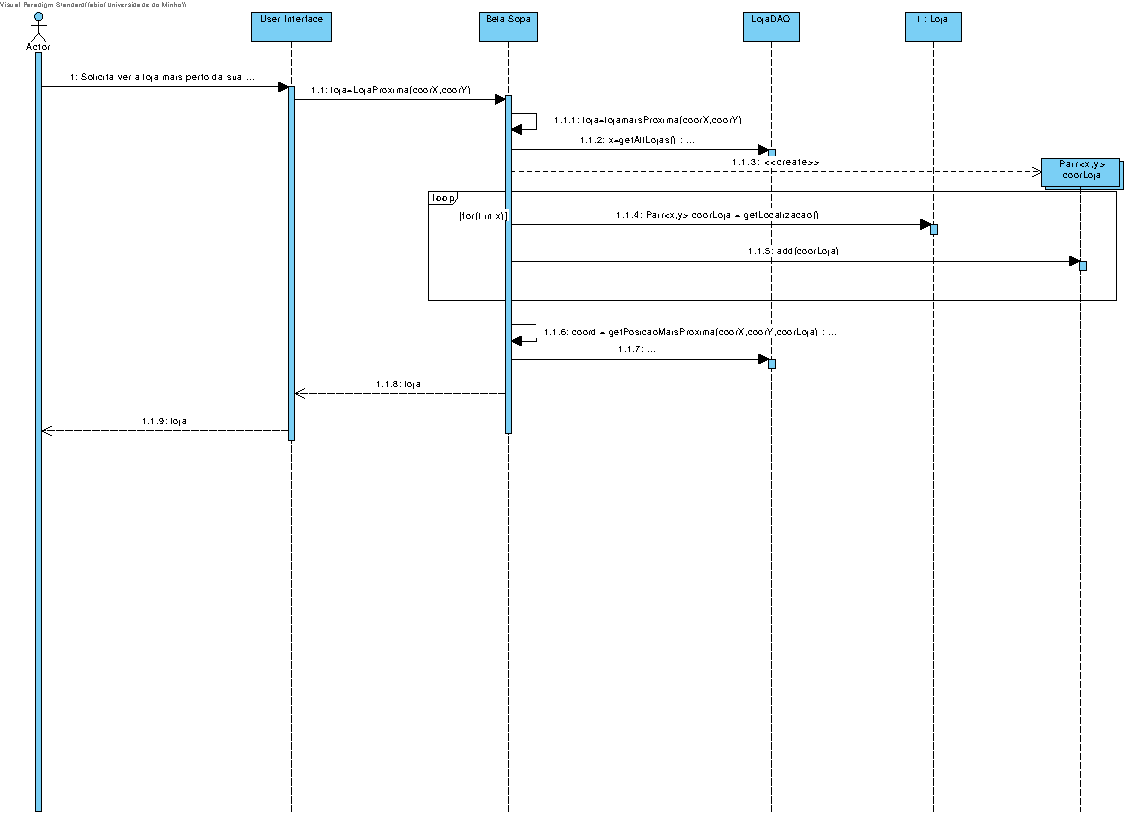
\includegraphics[width=\textwidth]{figures/10/Ver_loja_mais_perto.pdf}
   \caption{Diagrama de sequência para a visualização de lojas próximas.}
   \label{fig:negocio:DiagramaSequencia11}
 \end{figure}
 
 \begin{figure}[ht]
   \centering
   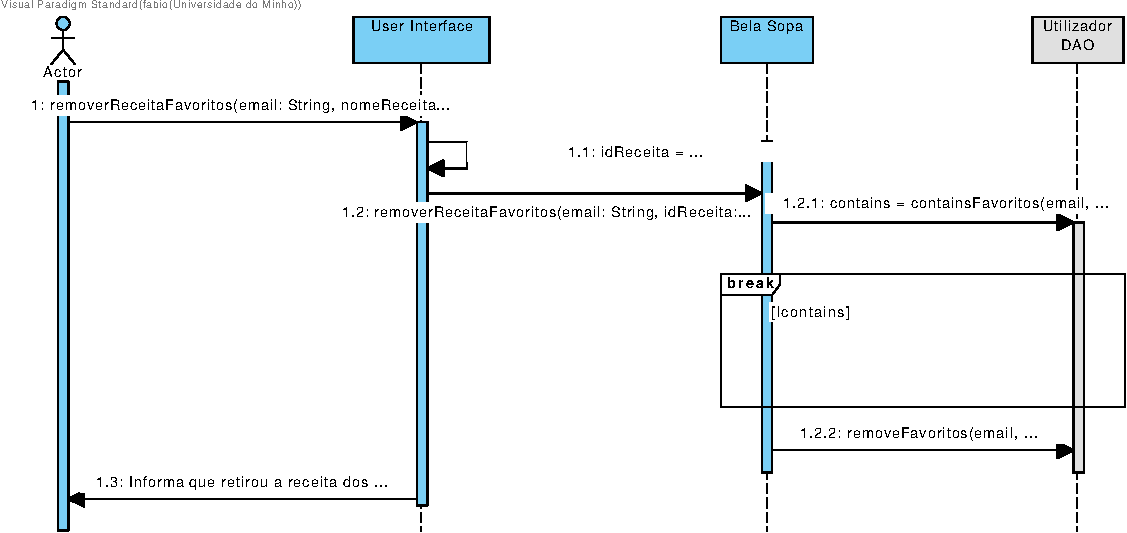
\includegraphics[width=\textwidth]{figures/10/Remover_receita_favoritos.pdf}
   \caption{Diagrama de sequência para a remoção de uma receita dos favoritos.}
   \label{fig:negocio:DiagramaSequencia12}
 \end{figure}

% ---------------------------------------------------------------------------- %


\end{document}

% ---------------------------------------------------------------------------- %
